\chapter{Arithmétique}
{https://sacado.xyz/qcm/parcours_show_course/0/117129}
{


 \begin{CpsCol}
\textbf{Les savoir-faire du parcours}
 \begin{itemize}
 \item Exploiter l'équation $y = f(x)$ d'une courbe : appartenance, calcul de coordonnées.
 \item  Modéliser par des fonctions des situations issues des mathématiques, des autres disciplines.
 \item Résoudre une équation du type $f(x) = k$ en choisissant une méthode adaptée :
graphique, algébrique, logicielle.
 \item Relier représentation graphique et tableau de variations.
 \item Déterminer graphiquement les extremums d'une fonction sur un intervalle.
 \item Exploiter un logiciel de géométrie dynamique ou de calcul formel, la calculatrice ou Python pour décrire
les variations d'une fonction donnée par une formule.
 \item Relier sens de variation, signe et droite représentative d'une fonction affine.
 \item Pour les fonctions affines, carré, inverse, racine carrée et cube, résoudre graphiquement ou algébriquement
une équation du type $f(x) = k$.
 \end{itemize}
 \end{CpsCol}

\begin{His}

 

\end{His}

 

\begin{ExoDec}{Chercher.}{1234}{1}{0}{0}{0}

 
 
\end{ExoDec}

}


\begin{pageCours}


\section{Généralités sur les fonctions}

\begin{DefT}{Notion de fonction} \index{Fonction!Antécédent}\index{Fonction!}\index{Fonction!Ensemble de définition}

\begin{minipage}{0.48\linewidth}
Définir une fonction $f$ d'un ensemble $\mathcal D$ de réels dans $\R$, c'est associer à chaque réel $x$ de $\mathcal D$ un
unique réel noté $f(x)$.
\begin{description}
\item On dit que  $\mathcal D$  est l'\textbf{ensemble de définition} de $f$. 
\item $f(x)$ est l'\textbf{image} de $x$ par $f$.
\item $x$ est un \textbf{antécédent} de $f(x)$ par $f$.
\end{description}
\end{minipage}
\begin{minipage}{0.48\linewidth}
\begin{center}
\definecolor{sqsqsq}{rgb}{0.12549019607843137,0.12549019607843137,0.12549019607843137}
\definecolor{ffqqqq}{rgb}{1.,0.,0.}
\begin{tikzpicture}[line cap=round,line join=round,>=triangle 45,x=1.0cm,y=1.0cm]
\clip(1.84,4.9) rectangle (9.52,7.);
\draw [color=ffqqqq] (4.,6.62)-- (7.,6.62);
\draw [color=ffqqqq] (7.,6.62)-- (7.,5.32);
\draw [color=ffqqqq] (7.,5.32)-- (4.,5.32);
\draw [color=ffqqqq] (4.,5.32)-- (4.,6.62);
\draw [-] (2.62,6.) -- (4.,6.);
\draw [->] (7.,5.98) -- (8.3,6.);
\draw [color=sqsqsq](2.44,6.25) node[anchor=north west] {|};
\draw [color=sqsqsq](4.58,6.2) node[anchor=north west] {fonction};
\draw [color=sqsqsq](6.34,6.2) node[anchor=north west] {$f$};
\draw [color=sqsqsq](2.06,6.2) node[anchor=north west] {$x$};
\draw [color=sqsqsq](8.36,6.2) node[anchor=north west] {$f(x)$};
\end{tikzpicture}
\end{center}
$f : D \longrightarrow \R$

$\quad x \mapsto f(x)$

Ce qui se lit : la fonction $f$ qui à $x$ associe $f(x)$.


\end{minipage}
\end{DefT}

\begin{Rqs}
La fonction se nomme par une lettre, généralement $f$, et peut être générée de 4 façons différentes.
\begin{itemize}
\item une expression algébrique notée $f(x)$ avec laquelle on calcule des images.
 \item une courbe, généralement appelée $\mathcal C_{f}$
\item un tableau de valeurs qui associe sur deux lignes, quelques valeurs et leurs images.
\item un algorithme, qui décrit les étapes de calcul pour obtenir $f(x)$
 \end{itemize}
 
\end{Rqs}
 
 
\subsection{Fonction générée par une expression algébrique}
 
\begin{DefT}{Expression algébrique d'une fonction}
Soit $f$ une fonction définie sur son domaine de définition $\mathcal D$.
L'expression algébrique de $f$ est la forme algébrique de $f(x)$.
\end{DefT}
 

\begin{MtT}{Déterminer algébriquement une image  par $f$}
Soit $f$ la fonction définie sur $\mathbb R$ par $f(x)= 2x^2 - 6x + 3$.

Pour déterminer l'image d'un nombre $a$ par $f$, il suffit de calculer $f(a)$.

L'image de $5$ par $f$ est $f(5)= 2\times 5^2 - 6\times 5 + 3 = 50-30+3 = 23$

L'image de $\sqrt{3}$ par $f$ est $f(\sqrt{3})= 2  \sqrt{2}^2 - 6  \sqrt{2} + 3 = 4-6\sqrt{2}+3 = 7-6\sqrt{2}$
\end{MtT}



\begin{MtT}{Déterminer algébriquement un antécédent par $f$}
Soit $f$ la fonction définie sur $\mathbb R$ par $f(x)= 2x^2 - 6x + 3$.

Pour déterminer le (ou les) antécédent(s) d'un nombre $a$ par $f$, il faut et il suffit de résoudre l'équation $f(x) = 3$.

$2x^2 - 6x + 3 = 3$

$2x^2 - 6x = 0$

$2x (x - 3) = 0$

$2x = 0$ ou $x - 3 = 0$ , $x = 0$ ou  $x = 3$. $\mathscr{S}=\left\lbrace 0;3\right\rbrace $. Les antécédents de 3 par $f$ sont 0 et 3.

\end{MtT}



\begin{Rq} 
Lorsque le domaine de définition n'est pas donné, l'expression algébrique $f(x)$ de la fonction $f$ permet de le déterminer.
\end{Rq} 


\end{pageCours}


\begin{pageAD} 
 

\Sf{Modéliser par des fonctions}

\begin{ExoCad}{Modéliser.}{1234}{0}{0}{0}{0}{0}
Soit $f$ la fonction qui à un coté $c$ d'un triangle équilatéral associe son périmètre. Définir $f$. \point{3}
\end{ExoCad} 


\begin{ExoCad}{Modéliser.}{1234}{0}{0}{0}{0}{0}
Pour une distance connue, la vitesse moyenne se définit en fonction du temps. La distance entre Toulon et Hyères est de 20km. Définir la fonction vitesse moyenne $v$. \point{2}
\end{ExoCad} 

\Sf{Déterminer les images par une fonction $f$.}

\begin{ExoCad}{Modéliser.}{1234}{0}{0}{0}{0}{0}

Soit $f$ la fonction définie sur $[0;+\infty[$ par $f(x)= 4x^2+3x$. Calculer

\begin{enumerate}
\item l'image de 2 par $f$, $f(2)=$\point{1}
\item l'image de $\dfrac{2}{3}$ par $f$, $f\left(\dfrac{2}{3}\right)=$\point{1}
\item l'image de $\sqrt{5}$ par $f$, $f\left(\sqrt{5}\right)=$\point{1}
\end{enumerate}
\end{ExoCad} 

 

\begin{ExoCad}{Modéliser.}{1234}{0}{0}{0}{0}{0}

Soit $f$ la fonction définie sur $]-\infty;1[$ par $f(x)= \dfrac{5}{x-1}$. 

\begin{enumerate}
\item Calculer l'image de $-2$ par $f$.  

\point{1}
\item Calculer l'image de $\dfrac{3}{7}$ par $f$. 

\point{2}
\end{enumerate}
\end{ExoCad}


 

\begin{ExoCad}{Modéliser.}{1234}{0}{0}{0}{0}{0}

Soit $g$ la fonction définie sur $\mathbb R$ par $g(x)=2x-1$. 

\begin{enumerate}
\item Déterminer un antécédent de $4$ par $g$.  

\point{2}
\item Déterminer un antécédent de $\dfrac{3}{4}$ par $g$.  

\point{2}
\end{enumerate}
\end{ExoCad}


\begin{ExoCad}{Modéliser.}{1234}{0}{0}{0}{0}{0}
Déterminer le domaine de définition de la fonction $f$ définie par $f(x)=\frac{3}{x-8}$. \point{2}
\end{ExoCad}

\end{pageAD} 


\begin{pageCours}

\subsection{Fonction représentée par une courbe}


\begin{DefT}{Représentation graphique}\index{Représentation graphique}\index{Équation de courbe}
Le plan est muni d'un repère (O ; I ; J). Soit $f$ une fonction définie sur l'ensemble $D$.\\
La \textbf{représentation graphique} ou courbe représentative $\mathscr{C}_f$ de la fonction $f$ dans le repère (O ; I ; J) est l'ensemble des points de coordonnées $(x ; f (x))$, où $x \in D$. Une équation de $\mathscr{C}_f$ est $y=f(x)$.
\end{DefT}

\begin{PpT}{Appartenance d'un point à une courbe}
Soit $f$ une fonction définie sur un ensemble $\mathcal{D}$ et $A(x_A,y_A)$ un point du plan.
\begin{enumerate}
\item Si le point $A$ appartient à la courbe $\mathscr{C}_f$ alors $y_A=f(x_A)$.
\item Réciproquement, si $y_A=f(x_A)$ alors le point $A$ appartient à la courbe $\mathscr{C}_f$. 
\end{enumerate}
\end{PpT}

\begin{Ex} 

Soit $f$ la fonction définie par $f(x)=5x^2+3x-1$.

\begin{minipage}{0.5\linewidth} 
Soit $A({\color{red}2};{\color{blue}25})$ un point du plan. 

$A$ appartient-il à la courbe de $f$ ?

$f({\color{red}2})=5\times 2^2+3\times 2-1={\color{blue}25}=y_A$ 

donc le point $A$ appartient à la courbe de $f$.  
\end{minipage}
\begin{minipage}{0.5\linewidth} 
Soit $B({\color{red}-1};{\color{blue}2})$ un point du plan.  

$B$ appartient-il à la courbe de $f$ ?

$f({\color{red}-1})=5\times ({\color{red}-1}^2+3\times ({\color{red}-1}-1=5-3-1={\color{blue}1}$ 

$f(x_B)\neq y_B$ donc $B$ n'appartient pas à la courbe de $f$.  
\end{minipage}
\end{Ex}




\begin{Rqs}
\begin{itemize}
\item Le tracé d'une courbe représentative est toujours approximatif : on construit un tableau de valeurs, on place les points correspondants dans un repère et on les relie par une courbe régulière.
\item On peut utiliser la calculatrice pour remplir un tableau de valeurs et tracer des courbes représentatives. 
\item Certaines fonctions ne sont connues que par leur courbe représentative
\end{itemize}
\end{Rqs}




\begin{MtT}{Déterminer graphiquement une image ou un antécédent par $f$}
\index{Lecture graphique!Image}\index{Lecture graphique!Antécédent}
On se reportera à la figure ci dessous
\begin{itemize}
\item L'image de $a$ est l'ordonnée du point de la courbe d'abscisse $a$.
\item Les antécédents de $b$ sont les abscisses des points de la courbe dont l'ordonnée est $b$.
\end{itemize}

\begin{minipage}{0.48\linewidth}
\textbf{Lecture d'image}

\definecolor{ffqqqq}{rgb}{1.,0.,0.}
\definecolor{qqwuqq}{rgb}{0.,0.39215686274509803,0.}
\definecolor{uuuuuu}{rgb}{0.26666666666666666,0.26666666666666666,0.26666666666666666}
\definecolor{xdxdff}{rgb}{0.49019607843137253,0.49019607843137253,1.}
\definecolor{ccqqqq}{rgb}{0.8,0.,0.}
\begin{tikzpicture}[line cap=round,line join=round,>=triangle 45,x=1.0cm,y=1.0cm]
\draw[->,color=black] (-1.2,0.) -- (6.54,0.);
\foreach \x in {-1.,1.,2.,3.,4.,5.,6.}
\draw[shift={(\x,0)},color=black] (0pt,2pt) -- (0pt,-2pt) node[below] {\footnotesize $\x$};
\draw[->,color=black] (0.,-0.58) -- (0.,4.1);
\foreach \y in {,1.,2.,3.,4.}
\draw[shift={(0,\y)},color=black] (2pt,0pt) -- (-2pt,0pt) node[left] {\footnotesize $\y$};
\draw[color=black] (0pt,-10pt) node[right] {\footnotesize $0$};
\clip(-1.2,-0.58) rectangle (6.54,4.1);
\draw[line width=1.2pt,color=ccqqqq] (0.02000202000000007,1.0333351288922137) -- (0.02000202000000007,1.0333351288922137);
\draw[line width=1.2pt,color=ccqqqq] (0.02000202000000007,1.0333351288922137) -- (0.0350020088527628,1.0468526628865917);
\draw[line width=1.2pt,color=ccqqqq] (0.0350020088527628,1.0468526628865917) -- (0.050001997705525526,1.0607417842661409);
\draw[line width=1.2pt,color=ccqqqq] (0.050001997705525526,1.0607417842661409) -- (0.06500198655828826,1.075007280091787);
\draw[line width=1.2pt,color=ccqqqq] (0.06500198655828826,1.075007280091787) -- (0.08000197541105099,1.0896537782492035);
\draw[line width=1.2pt,color=ccqqqq] (0.08000197541105099,1.0896537782492035) -- (0.09500196426381372,1.1046857321084331);
\draw[line width=1.2pt,color=ccqqqq] (0.09500196426381372,1.1046857321084331) -- (0.11000195311657644,1.120107404667603);
\draw[line width=1.2pt,color=ccqqqq] (0.11000195311657644,1.120107404667603) -- (0.12500194196933917,1.1359228521975857);
\draw[line width=1.2pt,color=ccqqqq] (0.12500194196933917,1.1359228521975857) -- (0.1400019308221019,1.1521359074080868);
\draw[line width=1.2pt,color=ccqqqq] (0.1400019308221019,1.1521359074080868) -- (0.15500191967486465,1.1687501621594936);
\draw[line width=1.2pt,color=ccqqqq] (0.15500191967486465,1.1687501621594936) -- (0.1700019085276274,1.1857689497488706);
\draw[line width=1.2pt,color=ccqqqq] (0.1700019085276274,1.1857689497488706) -- (0.18500189738039013,1.2031953268027384);
\draw[line width=1.2pt,color=ccqqqq] (0.18500189738039013,1.2031953268027384) -- (0.20000188623315288,1.2210320548137101);
\draw[line width=1.2pt,color=ccqqqq] (0.20000188623315288,1.2210320548137101) -- (0.21500187508591562,1.2392815813626485);
\draw[line width=1.2pt,color=ccqqqq] (0.21500187508591562,1.2392815813626485) -- (0.23000186393867836,1.2579460210727733);
\draw[line width=1.2pt,color=ccqqqq] (0.23000186393867836,1.2579460210727733) -- (0.2450018527914411,1.2770271363470083);
\draw[line width=1.2pt,color=ccqqqq] (0.2450018527914411,1.2770271363470083) -- (0.2600018416442038,1.2965263179448447);
\draw[line width=1.2pt,color=ccqqqq] (0.2600018416442038,1.2965263179448447) -- (0.2750018304969665,1.3164445654600376);
\draw[line width=1.2pt,color=ccqqqq] (0.2750018304969665,1.3164445654600376) -- (0.29000181934972924,1.3367824677655373);
\draw[line width=1.2pt,color=ccqqqq] (0.29000181934972924,1.3367824677655373) -- (0.30500180820249195,1.357540183497144);
\draw[line width=1.2pt,color=ccqqqq] (0.30500180820249195,1.357540183497144) -- (0.32000179705525467,1.3787174216524065);
\draw[line width=1.2pt,color=ccqqqq] (0.32000179705525467,1.3787174216524065) -- (0.3350017859080174,1.4003134223862463);
\draw[line width=1.2pt,color=ccqqqq] (0.3350017859080174,1.4003134223862463) -- (0.3500017747607801,1.422326938089602);
\draw[line width=1.2pt,color=ccqqqq] (0.3500017747607801,1.422326938089602) -- (0.3650017636135428,1.4447562148420192);
\draw[line width=1.2pt,color=ccqqqq] (0.3650017636135428,1.4447562148420192) -- (0.3800017524663055,1.4675989743334903);
\draw[line width=1.2pt,color=ccqqqq] (0.3800017524663055,1.4675989743334903) -- (0.39500174131906823,1.4908523963549363);
\draw[line width=1.2pt,color=ccqqqq] (0.39500174131906823,1.4908523963549363) -- (0.41000173017183095,1.5145131019604348);
\draw[line width=1.2pt,color=ccqqqq] (0.41000173017183095,1.5145131019604348) -- (0.42500171902459366,1.5385771374075912);
\draw[line width=1.2pt,color=ccqqqq] (0.42500171902459366,1.5385771374075912) -- (0.4400017078773564,1.5630399589852422);
\draw[line width=1.2pt,color=ccqqqq] (0.4400017078773564,1.5630399589852422) -- (0.4550016967301191,1.587896418839931);
\draw[line width=1.2pt,color=ccqqqq] (0.4550016967301191,1.587896418839931) -- (0.4700016855828818,1.613140751914209);
\draw[line width=1.2pt,color=ccqqqq] (0.4700016855828818,1.613140751914209) -- (0.4850016744356445,1.6387665641107505);
\draw[line width=1.2pt,color=ccqqqq] (0.4850016744356445,1.6387665641107505) -- (0.5000016632884072,1.6647668217964553);
\draw[line width=1.2pt,color=ccqqqq] (0.5000016632884072,1.6647668217964553) -- (0.51500165214117,1.6911338427600933);
\draw[line width=1.2pt,color=ccqqqq] (0.51500165214117,1.6911338427600933) -- (0.5300016409939328,1.71785928873556);
\draw[line width=1.2pt,color=ccqqqq] (0.5300016409939328,1.71785928873556) -- (0.5450016298466955,1.7449341596004109);
\draw[line width=1.2pt,color=ccqqqq] (0.5450016298466955,1.7449341596004109) -- (0.5600016186994583,1.7723487893559928);
\draw[line width=1.2pt,color=ccqqqq] (0.5600016186994583,1.7723487893559928) -- (0.5750016075522211,1.8000928439911317);
\draw[line width=1.2pt,color=ccqqqq] (0.5750016075522211,1.8000928439911317) -- (0.5900015964049838,1.8281553213259696);
\draw[line width=1.2pt,color=ccqqqq] (0.5900015964049838,1.8281553213259696) -- (0.6050015852577466,1.8565245529261258);
\draw[line width=1.2pt,color=ccqqqq] (0.6050015852577466,1.8565245529261258) -- (0.6200015741105094,1.8851882081698808);
\draw[line width=1.2pt,color=ccqqqq] (0.6200015741105094,1.8851882081698808) -- (0.6350015629632721,1.9141333005425774);
\draw[line width=1.2pt,color=ccqqqq] (0.6350015629632721,1.9141333005425774) -- (0.6500015518160349,1.9433461962228766);
\draw[line width=1.2pt,color=ccqqqq] (0.6500015518160349,1.9433461962228766) -- (0.6650015406687977,1.9728126250149511);
\draw[line width=1.2pt,color=ccqqqq] (0.6650015406687977,1.9728126250149511) -- (0.6800015295215605,2.002517693669182);
\draw[line width=1.2pt,color=ccqqqq] (0.6800015295215605,2.002517693669182) -- (0.6950015183743232,2.0324459016215064);
\draw[line width=1.2pt,color=ccqqqq] (0.6950015183743232,2.0324459016215064) -- (0.710001507227086,2.0625811591682885);
\draw[line width=1.2pt,color=ccqqqq] (0.710001507227086,2.0625811591682885) -- (0.7250014960798488,2.0929068080795825);
\draw[line width=1.2pt,color=ccqqqq] (0.7250014960798488,2.0929068080795825) -- (0.7400014849326115,2.1234056446389857);
\draw[line width=1.2pt,color=ccqqqq] (0.7400014849326115,2.1234056446389857) -- (0.7550014737853743,2.154059945083057);
\draw[line width=1.2pt,color=ccqqqq] (0.7550014737853743,2.154059945083057) -- (0.7700014626381371,2.18485149339765);
\draw[line width=1.2pt,color=ccqqqq] (0.7700014626381371,2.18485149339765) -- (0.7850014514908998,2.215761611412598);
\draw[line width=1.2pt,color=ccqqqq] (0.7850014514908998,2.215761611412598) -- (0.8000014403436626,2.2467711911201036);
\draw[line width=1.2pt,color=ccqqqq] (0.8000014403436626,2.2467711911201036) -- (0.8150014291964254,2.2778607291261768);
\draw[line width=1.2pt,color=ccqqqq] (0.8150014291964254,2.2778607291261768) -- (0.8300014180491881,2.3090103631285572);
\draw[line width=1.2pt,color=ccqqqq] (0.8300014180491881,2.3090103631285572) -- (0.8450014069019509,2.340199910299052);
\draw[line width=1.2pt,color=ccqqqq] (0.8450014069019509,2.340199910299052) -- (0.8600013957547137,2.3714089074331723);
\draw[line width=1.2pt,color=ccqqqq] (0.8600013957547137,2.3714089074331723) -- (0.8750013846074765,2.4026166527156056);
\draw[line width=1.2pt,color=ccqqqq] (0.8750013846074765,2.4026166527156056) -- (0.8900013734602392,2.43380224893654);
\draw[line width=1.2pt,color=ccqqqq] (0.8900013734602392,2.43380224893654) -- (0.905001362313002,2.464944647981332);
\draw[line width=1.2pt,color=ccqqqq] (0.905001362313002,2.464944647981332) -- (0.9200013511657648,2.496022696404641);
\draw[line width=1.2pt,color=ccqqqq] (0.9200013511657648,2.496022696404641) -- (0.9350013400185275,2.527015181890066);
\draw[line width=1.2pt,color=ccqqqq] (0.9350013400185275,2.527015181890066) -- (0.9500013288712903,2.557900880387663);
\draw[line width=1.2pt,color=ccqqqq] (0.9500013288712903,2.557900880387663) -- (0.9650013177240531,2.5886586037145913);
\draw[line width=1.2pt,color=ccqqqq] (0.9650013177240531,2.5886586037145913) -- (0.9800013065768158,2.6192672473986587);
\draw[line width=1.2pt,color=ccqqqq] (0.9800013065768158,2.6192672473986587) -- (0.9950012954295786,2.649705838540742);
\draw[line width=1.2pt,color=ccqqqq] (0.9950012954295786,2.649705838540742) -- (1.0100012842823414,2.6799535834700716);
\draw[line width=1.2pt,color=ccqqqq] (1.0100012842823414,2.6799535834700716) -- (1.0250012731351041,2.709989914966185);
\draw[line width=1.2pt,color=ccqqqq] (1.0250012731351041,2.709989914966185) -- (1.040001261987867,2.7397945388229794);
\draw[line width=1.2pt,color=ccqqqq] (1.040001261987867,2.7397945388229794) -- (1.0550012508406297,2.769347479533794);
\draw[line width=1.2pt,color=ccqqqq] (1.0550012508406297,2.769347479533794) -- (1.0700012396933924,2.798629124881675);
\draw[line width=1.2pt,color=ccqqqq] (1.0700012396933924,2.798629124881675) -- (1.0850012285461552,2.8276202692260393);
\draw[line width=1.2pt,color=ccqqqq] (1.0850012285461552,2.8276202692260393) -- (1.100001217398918,2.8563021552855856);
\draw[line width=1.2pt,color=ccqqqq] (1.100001217398918,2.8563021552855856) -- (1.1150012062516808,2.8846565142276255);
\draw[line width=1.2pt,color=ccqqqq] (1.1150012062516808,2.8846565142276255) -- (1.1300011951044435,2.912665603885687);
\draw[line width=1.2pt,color=ccqqqq] (1.1300011951044435,2.912665603885687) -- (1.1450011839572063,2.940312244940369);
\draw[line width=1.2pt,color=ccqqqq] (1.1450011839572063,2.940312244940369) -- (1.160001172809969,2.9675798549126813);
\draw[line width=1.2pt,color=ccqqqq] (1.160001172809969,2.9675798549126813) -- (1.1750011616627318,2.994452479834413);
\draw[line width=1.2pt,color=ccqqqq] (1.1750011616627318,2.994452479834413) -- (1.1900011505154946,3.0209148234762777);
\draw[line width=1.2pt,color=ccqqqq] (1.1900011505154946,3.0209148234762777) -- (1.2050011393682574,3.046952274031464);
\draw[line width=1.2pt,color=ccqqqq] (1.2050011393682574,3.046952274031464) -- (1.2200011282210201,3.072550928169613);
\draw[line width=1.2pt,color=ccqqqq] (1.2200011282210201,3.072550928169613) -- (1.235001117073783,3.097697612393995);
\draw[line width=1.2pt,color=ccqqqq] (1.235001117073783,3.097697612393995) -- (1.2500011059265457,3.1223799016525424);
\draw[line width=1.2pt,color=ccqqqq] (1.2500011059265457,3.1223799016525424) -- (1.2650010947793084,3.1465861351712436);
\draw[line width=1.2pt,color=ccqqqq] (1.2650010947793084,3.1465861351712436) -- (1.2800010836320712,3.170305429496081);
\draw[line width=1.2pt,color=ccqqqq] (1.2800010836320712,3.170305429496081) -- (1.295001072484834,3.19352768874697);
\draw[line width=1.2pt,color=ccqqqq] (1.295001072484834,3.19352768874697) -- (1.3100010613375968,3.2162436121039275);
\draw[line width=1.2pt,color=ccqqqq] (1.3100010613375968,3.2162436121039275) -- (1.3250010501903595,3.2384446985617794);
\draw[line width=1.2pt,color=ccqqqq] (1.3250010501903595,3.2384446985617794) -- (1.3400010390431223,3.260123249005038);
\draw[line width=1.2pt,color=ccqqqq] (1.3400010390431223,3.260123249005038) -- (1.355001027895885,3.281272365668913);
\draw[line width=1.2pt,color=ccqqqq] (1.355001027895885,3.281272365668913) -- (1.3700010167486478,3.3018859490658063);
\draw[line width=1.2pt,color=ccqqqq] (1.3700010167486478,3.3018859490658063) -- (1.3850010056014106,3.3219586924688764);
\draw[line width=1.2pt,color=ccqqqq] (1.3850010056014106,3.3219586924688764) -- (1.4000009944541734,3.3414860740553234);
\draw[line width=1.2pt,color=ccqqqq] (1.4000009944541734,3.3414860740553234) -- (1.4150009833069361,3.360464346821912);
\draw[line width=1.2pt,color=ccqqqq] (1.4150009833069361,3.360464346821912) -- (1.430000972159699,3.378890526393823);
\draw[line width=1.2pt,color=ccqqqq] (1.430000972159699,3.378890526393823) -- (1.4450009610124617,3.396762376855241);
\draw[line width=1.2pt,color=ccqqqq] (1.4450009610124617,3.396762376855241) -- (1.4600009498652244,3.414078394736099);
\draw[line width=1.2pt,color=ccqqqq] (1.4600009498652244,3.414078394736099) -- (1.4750009387179872,3.4308377912941754);
\draw[line width=1.2pt,color=ccqqqq] (1.4750009387179872,3.4308377912941754) -- (1.49000092757075,3.447040473235208);
\draw[line width=1.2pt,color=ccqqqq] (1.49000092757075,3.447040473235208) -- (1.5050009164235127,3.462687022016026);
\draw[line width=1.2pt,color=ccqqqq] (1.5050009164235127,3.462687022016026) -- (1.5200009052762755,3.477778671876796);
\draw[line width=1.2pt,color=ccqqqq] (1.5200009052762755,3.477778671876796) -- (1.5350008941290383,3.492317286748513);
\draw[line width=1.2pt,color=ccqqqq] (1.5350008941290383,3.492317286748513) -- (1.550000882981801,3.5063053361808816);
\draw[line width=1.2pt,color=ccqqqq] (1.550000882981801,3.5063053361808816) -- (1.5650008718345638,3.5197458704336975);
\draw[line width=1.2pt,color=ccqqqq] (1.5650008718345638,3.5197458704336975) -- (1.5800008606873266,3.5326424948720256);
\draw[line width=1.2pt,color=ccqqqq] (1.5800008606873266,3.5326424948720256) -- (1.5950008495400894,3.5449993438017624);
\draw[line width=1.2pt,color=ccqqqq] (1.5950008495400894,3.5449993438017624) -- (1.6100008383928521,3.55682105387778);
\draw[line width=1.2pt,color=ccqqqq] (1.6100008383928521,3.55682105387778) -- (1.625000827245615,3.5681127372118286);
\draw[line width=1.2pt,color=ccqqqq] (1.625000827245615,3.5681127372118286) -- (1.6400008160983777,3.5788799543017804);
\draw[line width=1.2pt,color=ccqqqq] (1.6400008160983777,3.5788799543017804) -- (1.6550008049511404,3.5891286868977508);
\draw[line width=1.2pt,color=ccqqqq] (1.6550008049511404,3.5891286868977508) -- (1.6700007938039032,3.598865310914226);
\draw[line width=1.2pt,color=ccqqqq] (1.6700007938039032,3.598865310914226) -- (1.685000782656666,3.6080965694905713);
\draw[line width=1.2pt,color=ccqqqq] (1.685000782656666,3.6080965694905713) -- (1.7000007715094287,3.616829546295387);
\draw[line width=1.2pt,color=ccqqqq] (1.7000007715094287,3.616829546295387) -- (1.7150007603621915,3.625071639163038);
\draw[line width=1.2pt,color=ccqqqq] (1.7150007603621915,3.625071639163038) -- (1.7300007492149543,3.63283053414355);
\draw[line width=1.2pt,color=ccqqqq] (1.7300007492149543,3.63283053414355) -- (1.745000738067717,3.640114180039843);
\draw[line width=1.2pt,color=ccqqqq] (1.745000738067717,3.640114180039843) -- (1.7600007269204798,3.6469307634991366);
\draw[line width=1.2pt,color=ccqqqq] (1.7600007269204798,3.6469307634991366) -- (1.7750007157732426,3.6532886847183157);
\draw[line width=1.2pt,color=ccqqqq] (1.7750007157732426,3.6532886847183157) -- (1.7900007046260054,3.6591965338161034);
\draw[line width=1.2pt,color=ccqqqq] (1.7900007046260054,3.6591965338161034) -- (1.8050006934787681,3.6646630679182);
\draw[line width=1.2pt,color=ccqqqq] (1.8050006934787681,3.6646630679182) -- (1.820000682331531,3.6696971889950034);
\draw[line width=1.2pt,color=ccqqqq] (1.820000682331531,3.6696971889950034) -- (1.8350006711842937,3.6743079224853012);
\draw[line width=1.2pt,color=ccqqqq] (1.8350006711842937,3.6743079224853012) -- (1.8500006600370564,3.6785043967333264);
\draw[line width=1.2pt,color=ccqqqq] (1.8500006600370564,3.6785043967333264) -- (1.8650006488898192,3.6822958232609038);
\draw[line width=1.2pt,color=ccqqqq] (1.8650006488898192,3.6822958232609038) -- (1.880000637742582,3.6856914778910435);
\draw[line width=1.2pt,color=ccqqqq] (1.880000637742582,3.6856914778910435) -- (1.8950006265953447,3.6887006827343063);
\draw[line width=1.2pt,color=ccqqqq] (1.8950006265953447,3.6887006827343063) -- (1.9100006154481075,3.691332789044562);
\draw[line width=1.2pt,color=ccqqqq] (1.9100006154481075,3.691332789044562) -- (1.9250006043008703,3.6935971609464016);
\draw[line width=1.2pt,color=ccqqqq] (1.9250006043008703,3.6935971609464016) -- (1.940000593153633,3.6955031600324353);
\draw[line width=1.2pt,color=ccqqqq] (1.940000593153633,3.6955031600324353) -- (1.9550005820063958,3.6970601308250393);
\draw[line width=1.2pt,color=ccqqqq] (1.9550005820063958,3.6970601308250393) -- (1.9700005708591586,3.6982773870937407);
\draw[line width=1.2pt,color=ccqqqq] (1.9700005708591586,3.6982773870937407) -- (1.9850005597119214,3.6991641990164217);
\draw[line width=1.2pt,color=ccqqqq] (1.9850005597119214,3.6991641990164217) -- (2.000000548564684,3.699729781169811);
\draw[line width=1.2pt,color=ccqqqq] (2.000000548564684,3.699729781169811) -- (2.0150005374174467,3.6999832813323135);
\draw[line width=1.2pt,color=ccqqqq] (2.0150005374174467,3.6999832813323135) -- (2.0300005262702094,3.6999337700801442);
\draw[line width=1.2pt,color=ccqqqq] (2.0300005262702094,3.6999337700801442) -- (2.045000515122972,3.699590231155874);
\draw[line width=1.2pt,color=ccqqqq] (2.045000515122972,3.699590231155874) -- (2.060000503975735,3.6989615525869506);
\draw[line width=1.2pt,color=ccqqqq] (2.060000503975735,3.6989615525869506) -- (2.0750004928284977,3.6980565185304357);
\draw[line width=1.2pt,color=ccqqqq] (2.0750004928284977,3.6980565185304357) -- (2.0900004816812605,3.696883801819121);
\draw[line width=1.2pt,color=ccqqqq] (2.0900004816812605,3.696883801819121) -- (2.1050004705340233,3.695451957183331);
\draw[line width=1.2pt,color=ccqqqq] (2.1050004705340233,3.695451957183331) -- (2.120000459386786,3.6937694151220595);
\draw[line width=1.2pt,color=ccqqqq] (2.120000459386786,3.6937694151220595) -- (2.135000448239549,3.6918444763966294);
\draw[line width=1.2pt,color=ccqqqq] (2.135000448239549,3.6918444763966294) -- (2.1500004370923116,3.6896853071197677);
\draw[line width=1.2pt,color=ccqqqq] (2.1500004370923116,3.6896853071197677) -- (2.1650004259450744,3.687299934412854);
\draw[line width=1.2pt,color=ccqqqq] (2.1650004259450744,3.687299934412854) -- (2.180000414797837,3.6846962426041134);
\draw[line width=1.2pt,color=ccqqqq] (2.180000414797837,3.6846962426041134) -- (2.1950004036506,3.681881969940658);
\draw[line width=1.2pt,color=ccqqqq] (2.1950004036506,3.681881969940658) -- (2.2100003925033627,3.6788647057875483);
\draw[line width=1.2pt,color=ccqqqq] (2.2100003925033627,3.6788647057875483) -- (2.2250003813561254,3.6756518882873865);
\draw[line width=1.2pt,color=ccqqqq] (2.2250003813561254,3.6756518882873865) -- (2.240000370208888,3.6722508024544283);
\draw[line width=1.2pt,color=ccqqqq] (2.240000370208888,3.6722508024544283) -- (2.255000359061651,3.668668578677695);
\draw[line width=1.2pt,color=ccqqqq] (2.255000359061651,3.668668578677695) -- (2.2700003479144137,3.664912191608206);
\draw[line width=1.2pt,color=ccqqqq] (2.2700003479144137,3.664912191608206) -- (2.2850003367671765,3.6609884594060706);
\draw[line width=1.2pt,color=ccqqqq] (2.2850003367671765,3.6609884594060706) -- (2.3000003256199393,3.656904043323904);
\draw[line width=1.2pt,color=ccqqqq] (2.3000003256199393,3.656904043323904) -- (2.315000314472702,3.6526654476037743);
\draw[line width=1.2pt,color=ccqqqq] (2.315000314472702,3.6526654476037743) -- (2.330000303325465,3.6482790196656616);
\draw[line width=1.2pt,color=ccqqqq] (2.330000303325465,3.6482790196656616) -- (2.3450002921782276,3.6437509505662087);
\draw[line width=1.2pt,color=ccqqqq] (2.3450002921782276,3.6437509505662087) -- (2.3600002810309904,3.639087275707375);
\draw[line width=1.2pt,color=ccqqqq] (2.3600002810309904,3.639087275707375) -- (2.375000269883753,3.634293875775419);
\draw[line width=1.2pt,color=ccqqqq] (2.375000269883753,3.634293875775419) -- (2.390000258736516,3.629376477891493);
\draw[line width=1.2pt,color=ccqqqq] (2.390000258736516,3.629376477891493) -- (2.4050002475892787,3.6243406569559578);
\draw[line width=1.2pt,color=ccqqqq] (2.4050002475892787,3.6243406569559578) -- (2.4200002364420414,3.619191837169363);
\draw[line width=1.2pt,color=ccqqqq] (2.4200002364420414,3.619191837169363) -- (2.435000225294804,3.6139352937138796);
\draw[line width=1.2pt,color=ccqqqq] (2.435000225294804,3.6139352937138796) -- (2.450000214147567,3.608576154579775);
\draw[line width=1.2pt,color=ccqqqq] (2.450000214147567,3.608576154579775) -- (2.4650002030003297,3.6031194025223345);
\draw[line width=1.2pt,color=ccqqqq] (2.4650002030003297,3.6031194025223345) -- (2.4800001918530925,3.5975698771354256);
\draw[line width=1.2pt,color=ccqqqq] (2.4800001918530925,3.5975698771354256) -- (2.4950001807058553,3.5919322770286604);
\draw[line width=1.2pt,color=ccqqqq] (2.4950001807058553,3.5919322770286604) -- (2.510000169558618,3.586211162095877);
\draw[line width=1.2pt,color=ccqqqq] (2.510000169558618,3.586211162095877) -- (2.525000158411381,3.5804109558633774);
\draw[line width=1.2pt,color=ccqqqq] (2.525000158411381,3.5804109558633774) -- (2.5400001472641436,3.5745359479070764);
\draw[line width=1.2pt,color=ccqqqq] (2.5400001472641436,3.5745359479070764) -- (2.5550001361169064,3.568590296328387);
\draw[line width=1.2pt,color=ccqqqq] (2.5550001361169064,3.568590296328387) -- (2.570000124969669,3.5625780302793393);
\draw[line width=1.2pt,color=ccqqqq] (2.570000124969669,3.5625780302793393) -- (2.585000113822432,3.5565030525280488);
\draw[line width=1.2pt,color=ccqqqq] (2.585000113822432,3.5565030525280488) -- (2.6000001026751947,3.550369142056267);
\draw[line width=1.2pt,color=ccqqqq] (2.6000001026751947,3.550369142056267) -- (2.6150000915279574,3.5441799566813295);
\draw[line width=1.2pt,color=ccqqqq] (2.6150000915279574,3.5441799566813295) -- (2.63000008038072,3.537939035695348);
\draw[line width=1.2pt,color=ccqqqq] (2.63000008038072,3.537939035695348) -- (2.645000069233483,3.5316498025150844);
\draw[line width=1.2pt,color=ccqqqq] (2.645000069233483,3.5316498025150844) -- (2.6600000580862457,3.5253155673363583);
\draw[line width=1.2pt,color=ccqqqq] (2.6600000580862457,3.5253155673363583) -- (2.6750000469390085,3.518939529787418);
\draw[line width=1.2pt,color=ccqqqq] (2.6750000469390085,3.518939529787418) -- (2.6900000357917713,3.512524781576079);
\draw[line width=1.2pt,color=ccqqqq] (2.6900000357917713,3.512524781576079) -- (2.705000024644534,3.5060743091259257);
\draw[line width=1.2pt,color=ccqqqq] (2.705000024644534,3.5060743091259257) -- (2.720000013497297,3.4995909961972393);
\draw[line width=1.2pt,color=ccqqqq] (2.720000013497297,3.4995909961972393) -- (2.7350000023500596,3.493077626488729);
\draw[line width=1.2pt,color=ccqqqq] (2.7350000023500596,3.493077626488729) -- (2.7499999912028223,3.486536886216491);
\draw[line width=1.2pt,color=ccqqqq] (2.7499999912028223,3.486536886216491) -- (2.764999980055585,3.4799713666669723);
\draw[line width=1.2pt,color=ccqqqq] (2.764999980055585,3.4799713666669723) -- (2.779999968908348,3.4733835667210307);
\draw[line width=1.2pt,color=ccqqqq] (2.779999968908348,3.4733835667210307) -- (2.7949999577611107,3.4667758953464975);
\draw[line width=1.2pt,color=ccqqqq] (2.7949999577611107,3.4667758953464975) -- (2.8099999466138734,3.460150674056915);
\draw[line width=1.2pt,color=ccqqqq] (2.8099999466138734,3.460150674056915) -- (2.824999935466636,3.4535101393344085);
\draw[line width=1.2pt,color=ccqqqq] (2.824999935466636,3.4535101393344085) -- (2.839999924319399,3.4468564450148778);
\draw[line width=1.2pt,color=ccqqqq] (2.839999924319399,3.4468564450148778) -- (2.8549999131721617,3.440191664633944);
\draw[line width=1.2pt,color=ccqqqq] (2.8549999131721617,3.440191664633944) -- (2.8699999020249245,3.4335177937322947);
\draw[line width=1.2pt,color=ccqqqq] (2.8699999020249245,3.4335177937322947) -- (2.8849998908776873,3.426836752119268);
\draw[line width=1.2pt,color=ccqqqq] (2.8849998908776873,3.426836752119268) -- (2.89999987973045,3.4201503860937077);
\draw[line width=1.2pt,color=ccqqqq] (2.89999987973045,3.4201503860937077) -- (2.914999868583213,3.4134604706212963);
\draw[line width=1.2pt,color=ccqqqq] (2.914999868583213,3.4134604706212963) -- (2.9299998574359756,3.406768711467723);
\draw[line width=1.2pt,color=ccqqqq] (2.9299998574359756,3.406768711467723) -- (2.9449998462887383,3.4000767472872013);
\draw[line width=1.2pt,color=ccqqqq] (2.9449998462887383,3.4000767472872013) -- (2.959999835141501,3.3933861516659833);
\draw[line width=1.2pt,color=ccqqqq] (2.959999835141501,3.3933861516659833) -- (2.974999823994264,3.3866984351206373);
\draw[line width=1.2pt,color=ccqqqq] (2.974999823994264,3.3866984351206373) -- (2.9899998128470267,3.3800150470509793);
\draw[line width=1.2pt,color=ccqqqq] (2.9899998128470267,3.3800150470509793) -- (3.0049998016997894,3.3733373776476503);
\draw[line width=1.2pt,color=ccqqqq] (3.0049998016997894,3.3733373776476503) -- (3.019999790552552,3.366666759754422);
\draw[line width=1.2pt,color=ccqqqq] (3.019999790552552,3.366666759754422) -- (3.034999779405315,3.360004470685408);
\draw[line width=1.2pt,color=ccqqqq] (3.034999779405315,3.360004470685408) -- (3.0499997682580777,3.353351733997437);
\draw[line width=1.2pt,color=ccqqqq] (3.0499997682580777,3.353351733997437) -- (3.0649997571108405,3.346709721217908);
\draw[line width=1.2pt,color=ccqqqq] (3.0649997571108405,3.346709721217908) -- (3.0799997459636033,3.3400795535285246);
\draw[line width=1.2pt,color=ccqqqq] (3.0799997459636033,3.3400795535285246) -- (3.094999734816366,3.333462303405348);
\draw[line width=1.2pt,color=ccqqqq] (3.094999734816366,3.333462303405348) -- (3.109999723669129,3.326858996215683);
\draw[line width=1.2pt,color=ccqqqq] (3.109999723669129,3.326858996215683) -- (3.1249997125218916,3.3202706117723295);
\draw[line width=1.2pt,color=ccqqqq] (3.1249997125218916,3.3202706117723295) -- (3.1399997013746543,3.3136980858457967);
\draw[line width=1.2pt,color=ccqqqq] (3.1399997013746543,3.3136980858457967) -- (3.154999690227417,3.307142311635106);
\draw[line width=1.2pt,color=ccqqqq] (3.154999690227417,3.307142311635106) -- (3.16999967908018,3.3006041411978266);
\draw[line width=1.2pt,color=ccqqqq] (3.16999967908018,3.3006041411978266) -- (3.1849996679329426,3.2940843868400425);
\draw[line width=1.2pt,color=ccqqqq] (3.1849996679329426,3.2940843868400425) -- (3.1999996567857054,3.2875838224669462);
\draw[line width=1.2pt,color=ccqqqq] (3.1999996567857054,3.2875838224669462) -- (3.214999645638468,3.2811031848947896);
\draw[line width=1.2pt,color=ccqqqq] (3.214999645638468,3.2811031848947896) -- (3.229999634491231,3.2746431751249316);
\draw[line width=1.2pt,color=ccqqqq] (3.229999634491231,3.2746431751249316) -- (3.2449996233439937,3.268204459580743);
\draw[line width=1.2pt,color=ccqqqq] (3.2449996233439937,3.268204459580743) -- (3.2599996121967565,3.261787671308129);
\draw[line width=1.2pt,color=ccqqqq] (3.2599996121967565,3.261787671308129) -- (3.2749996010495193,3.2553934111404477);
\draw[line width=1.2pt,color=ccqqqq] (3.2749996010495193,3.2553934111404477) -- (3.289999589902282,3.2490222488285996);
\draw[line width=1.2pt,color=ccqqqq] (3.289999589902282,3.2490222488285996) -- (3.304999578755045,3.242674724137073);
\draw[line width=1.2pt,color=ccqqqq] (3.304999578755045,3.242674724137073) -- (3.3199995676078076,3.2363513479067283);
\draw[line width=1.2pt,color=ccqqqq] (3.3199995676078076,3.2363513479067283) -- (3.3349995564605703,3.2300526030851033);
\draw[line width=1.2pt,color=ccqqqq] (3.3349995564605703,3.2300526030851033) -- (3.349999545313333,3.2237789457250194);
\draw[line width=1.2pt,color=ccqqqq] (3.349999545313333,3.2237789457250194) -- (3.364999534166096,3.217530805952266);
\draw[line width=1.2pt,color=ccqqqq] (3.364999534166096,3.217530805952266) -- (3.3799995230188586,3.2113085889031354);
\draw[line width=1.2pt,color=ccqqqq] (3.3799995230188586,3.2113085889031354) -- (3.3949995118716214,3.2051126756325727);
\draw[line width=1.2pt,color=ccqqqq] (3.3949995118716214,3.2051126756325727) -- (3.409999500724384,3.1989434239936942);
\draw[line width=1.2pt,color=ccqqqq] (3.409999500724384,3.1989434239936942) -- (3.424999489577147,3.192801169489434);
\draw[line width=1.2pt,color=ccqqqq] (3.424999489577147,3.192801169489434) -- (3.4399994784299097,3.186686226097043);
\draw[line width=1.2pt,color=ccqqqq] (3.4399994784299097,3.186686226097043) -- (3.4549994672826725,3.1805988870661874);
\draw[line width=1.2pt,color=ccqqqq] (3.4549994672826725,3.1805988870661874) -- (3.4699994561354353,3.174539425691352);
\draw[line width=1.2pt,color=ccqqqq] (3.4699994561354353,3.174539425691352) -- (3.484999444988198,3.168508096059261);
\draw[line width=1.2pt,color=ccqqqq] (3.484999444988198,3.168508096059261) -- (3.499999433840961,3.1625051337720187);
\draw[line width=1.2pt,color=ccqqqq] (3.499999433840961,3.1625051337720187) -- (3.5149994226937236,3.156530756646637);
\draw[line width=1.2pt,color=ccqqqq] (3.5149994226937236,3.156530756646637) -- (3.5299994115464863,3.150585165391642);
\draw[line width=1.2pt,color=ccqqqq] (3.5299994115464863,3.150585165391642) -- (3.544999400399249,3.1446685442614033);
\draw[line width=1.2pt,color=ccqqqq] (3.544999400399249,3.1446685442614033) -- (3.559999389252012,3.13878106168883);
\draw[line width=1.2pt,color=ccqqqq] (3.559999389252012,3.13878106168883) -- (3.5749993781047746,3.1329228708970795);
\draw[line width=1.2pt,color=ccqqqq] (3.5749993781047746,3.1329228708970795) -- (3.5899993669575374,3.127094110490882);
\draw[line width=1.2pt,color=ccqqqq] (3.5899993669575374,3.127094110490882) -- (3.6049993558103,3.1212949050280896);
\draw[line width=1.2pt,color=ccqqqq] (3.6049993558103,3.1212949050280896) -- (3.619999344663063,3.115525365572048);
\draw[line width=1.2pt,color=ccqqqq] (3.619999344663063,3.115525365572048) -- (3.6349993335158257,3.1097855902253624);
\draw[line width=1.2pt,color=ccqqqq] (3.6349993335158257,3.1097855902253624) -- (3.6499993223685885,3.104075664645615);
\draw[line width=1.2pt,color=ccqqqq] (3.6499993223685885,3.104075664645615) -- (3.6649993112213513,3.0983956625435995);
\draw[line width=1.2pt,color=ccqqqq] (3.6649993112213513,3.0983956625435995) -- (3.679999300074114,3.0927456461645972);
\draw[line width=1.2pt,color=ccqqqq] (3.679999300074114,3.0927456461645972) -- (3.694999288926877,3.0871256667532174);
\draw[line width=1.2pt,color=ccqqqq] (3.694999288926877,3.0871256667532174) -- (3.7099992777796396,3.0815357650023243);
\draw[line width=1.2pt,color=ccqqqq] (3.7099992777796396,3.0815357650023243) -- (3.7249992666324023,3.0759759714865282);
\draw[line width=1.2pt,color=ccqqqq] (3.7249992666324023,3.0759759714865282) -- (3.739999255485165,3.0704463070807453);
\draw[line width=1.2pt,color=ccqqqq] (3.739999255485165,3.0704463070807453) -- (3.754999244337928,3.0649467833642774);
\draw[line width=1.2pt,color=ccqqqq] (3.754999244337928,3.0649467833642774) -- (3.7699992331906906,3.0594774030108827);
\draw[line width=1.2pt,color=ccqqqq] (3.7699992331906906,3.0594774030108827) -- (3.7849992220434534,3.0540381601652795);
\draw[line width=1.2pt,color=ccqqqq] (3.7849992220434534,3.0540381601652795) -- (3.799999210896216,3.04862904080651);
\draw[line width=1.2pt,color=ccqqqq] (3.799999210896216,3.04862904080651) -- (3.814999199748979,3.0432500230985973);
\draw[line width=1.2pt,color=ccqqqq] (3.814999199748979,3.0432500230985973) -- (3.8299991886017417,3.0379010777288915);
\draw[line width=1.2pt,color=ccqqqq] (3.8299991886017417,3.0379010777288915) -- (3.8449991774545045,3.032582168234511);
\draw[line width=1.2pt,color=ccqqqq] (3.8449991774545045,3.032582168234511) -- (3.8599991663072672,3.0272932513172646);
\draw[line width=1.2pt,color=ccqqqq] (3.8599991663072672,3.0272932513172646) -- (3.87499915516003,3.022034277147424);
\draw[line width=1.2pt,color=ccqqqq] (3.87499915516003,3.022034277147424) -- (3.889999144012793,3.0168051896567127);
\draw[line width=1.2pt,color=ccqqqq] (3.889999144012793,3.0168051896567127) -- (3.9049991328655556,3.0116059268208724);
\draw[line width=1.2pt,color=ccqqqq] (3.9049991328655556,3.0116059268208724) -- (3.9199991217183183,3.0064364209321317);
\draw[line width=1.2pt,color=ccqqqq] (3.9199991217183183,3.0064364209321317) -- (3.934999110571081,3.0012965988619293);
\draw[line width=1.2pt,color=ccqqqq] (3.934999110571081,3.0012965988619293) -- (3.949999099423844,2.996186382314201);
\draw[line width=1.2pt,color=ccqqqq] (3.949999099423844,2.996186382314201) -- (3.9649990882766066,2.9911056880695464);
\draw[line width=1.2pt,color=ccqqqq] (3.9649990882766066,2.9911056880695464) -- (3.9799990771293694,2.9860544282205805);
\draw[line width=1.2pt,color=ccqqqq] (3.9799990771293694,2.9860544282205805) -- (3.994999065982132,2.9810325103987623);
\draw[line width=1.2pt,color=ccqqqq] (3.994999065982132,2.9810325103987623) -- (4.0099990548348945,2.9760398379929835);
\draw[line width=1.2pt,color=ccqqqq] (4.0099990548348945,2.9760398379929835) -- (4.024999043687657,2.9710763103601954);
\draw[line width=1.2pt,color=ccqqqq] (4.024999043687657,2.9710763103601954) -- (4.03999903254042,2.96614182302834);
\draw[line width=1.2pt,color=ccqqqq] (4.03999903254042,2.96614182302834) -- (4.054999021393183,2.9612362678918487);
\draw[line width=1.2pt,color=ccqqqq] (4.054999021393183,2.9612362678918487) -- (4.069999010245946,2.956359533399947);
\draw[line width=1.2pt,color=ccqqqq] (4.069999010245946,2.956359533399947) -- (4.084998999098708,2.951511504738023);
\draw[line width=1.2pt,color=ccqqqq] (4.084998999098708,2.951511504738023) -- (4.099998987951471,2.946692064002288);
\draw[line width=1.2pt,color=ccqqqq] (4.099998987951471,2.946692064002288) -- (4.114998976804234,2.941901090367951);
\draw[line width=1.2pt,color=ccqqqq] (4.114998976804234,2.941901090367951) -- (4.129998965656997,2.9371384602511403);
\draw[line width=1.2pt,color=ccqqqq] (4.129998965656997,2.9371384602511403) -- (4.144998954509759,2.9324040474647726);
\draw[line width=1.2pt,color=ccqqqq] (4.144998954509759,2.9324040474647726) -- (4.159998943362522,2.9276977233685852);
\draw[line width=1.2pt,color=ccqqqq] (4.159998943362522,2.9276977233685852) -- (4.174998932215285,2.9230193570135268);
\draw[line width=1.2pt,color=ccqqqq] (4.174998932215285,2.9230193570135268) -- (4.189998921068048,2.918368815280701);
\draw[line width=1.2pt,color=ccqqqq] (4.189998921068048,2.918368815280701) -- (4.2049989099208105,2.9137459630150464);
\draw[line width=1.2pt,color=ccqqqq] (4.2049989099208105,2.9137459630150464) -- (4.219998898773573,2.9091506631539445);
\draw[line width=1.2pt,color=ccqqqq] (4.219998898773573,2.9091506631539445) -- (4.234998887626336,2.904582776850912);
\draw[line width=1.2pt,color=ccqqqq] (4.234998887626336,2.904582776850912) -- (4.249998876479099,2.90004216359457);
\draw[line width=1.2pt,color=ccqqqq] (4.249998876479099,2.90004216359457) -- (4.264998865331862,2.8955286813230297);
\draw[line width=1.2pt,color=ccqqqq] (4.264998865331862,2.8955286813230297) -- (4.279998854184624,2.8910421865338742);
\draw[line width=1.2pt,color=ccqqqq] (4.279998854184624,2.8910421865338742) -- (4.294998843037387,2.8865825343898734);
\draw[line width=1.2pt,color=ccqqqq] (4.294998843037387,2.8865825343898734) -- (4.30999883189015,2.8821495788205893);
\draw[line width=1.2pt,color=ccqqqq] (4.30999883189015,2.8821495788205893) -- (4.324998820742913,2.8777431726200113);
\draw[line width=1.2pt,color=ccqqqq] (4.324998820742913,2.8777431726200113) -- (4.339998809595675,2.8733631675403606);
\draw[line width=1.2pt,color=ccqqqq] (4.339998809595675,2.8733631675403606) -- (4.354998798448438,2.869009414382195);
\draw[line width=1.2pt,color=ccqqqq] (4.354998798448438,2.869009414382195) -- (4.369998787301201,2.8646817630809505);
\draw[line width=1.2pt,color=ccqqqq] (4.369998787301201,2.8646817630809505) -- (4.384998776153964,2.860380062790033);
\draw[line width=1.2pt,color=ccqqqq] (4.384998776153964,2.860380062790033) -- (4.3999987650067265,2.8561041619605927);
\draw[line width=1.2pt,color=ccqqqq] (4.3999987650067265,2.8561041619605927) -- (4.414998753859489,2.851853908418091);
\draw[line width=1.2pt,color=ccqqqq] (4.414998753859489,2.851853908418091) -- (4.429998742712252,2.8476291494357735);
\draw[line width=1.2pt,color=ccqqqq] (4.429998742712252,2.8476291494357735) -- (4.444998731565015,2.8434297318051582);
\draw[line width=1.2pt,color=ccqqqq] (4.444998731565015,2.8434297318051582) -- (4.459998720417778,2.8392555019036494);
\draw[line width=1.2pt,color=ccqqqq] (4.459998720417778,2.8392555019036494) -- (4.47499870927054,2.8351063057593677);
\draw[line width=1.2pt,color=ccqqqq] (4.47499870927054,2.8351063057593677) -- (4.489998698123303,2.8309819891133063);
\draw[line width=1.2pt,color=ccqqqq] (4.489998698123303,2.8309819891133063) -- (4.504998686976066,2.8268823974789035);
\draw[line width=1.2pt,color=ccqqqq] (4.504998686976066,2.8268823974789035) -- (4.519998675828829,2.82280737619912);
\draw[line width=1.2pt,color=ccqqqq] (4.519998675828829,2.82280737619912) -- (4.534998664681591,2.818756770501113);
\draw[line width=1.2pt,color=ccqqqq] (4.534998664681591,2.818756770501113) -- (4.549998653534354,2.814730425548598);
\draw[line width=1.2pt,color=ccqqqq] (4.549998653534354,2.814730425548598) -- (4.564998642387117,2.8107281864919704);
\draw[line width=1.2pt,color=ccqqqq] (4.564998642387117,2.8107281864919704) -- (4.57999863123988,2.8067498985162693);
\draw[line width=1.2pt,color=ccqqqq] (4.57999863123988,2.8067498985162693) -- (4.5949986200926425,2.8027954068870744);
\draw[line width=1.2pt,color=ccqqqq] (4.5949986200926425,2.8027954068870744) -- (4.609998608945405,2.7988645569943875);
\draw[line width=1.2pt,color=ccqqqq] (4.609998608945405,2.7988645569943875) -- (4.624998597798168,2.794957194394589);
\draw[line width=1.2pt,color=ccqqqq] (4.624998597798168,2.794957194394589) -- (4.639998586650931,2.7910731648505323);
\draw[line width=1.2pt,color=ccqqqq] (4.639998586650931,2.7910731648505323) -- (4.654998575503694,2.7872123143698415);
\draw[line width=1.2pt,color=ccqqqq] (4.654998575503694,2.7872123143698415) -- (4.669998564356456,2.7833744892414822);
\draw[line width=1.2pt,color=ccqqqq] (4.669998564356456,2.7833744892414822) -- (4.684998553209219,2.7795595360706606);
\draw[line width=1.2pt,color=ccqqqq] (4.684998553209219,2.7795595360706606) -- (4.699998542061982,2.775767301812121);
\draw[line width=1.2pt,color=ccqqqq] (4.699998542061982,2.775767301812121) -- (4.714998530914745,2.7719976338018943);
\draw[line width=1.2pt,color=ccqqqq] (4.714998530914745,2.7719976338018943) -- (4.729998519767507,2.7682503797875486);
\draw[line width=1.2pt,color=ccqqqq] (4.729998519767507,2.7682503797875486) -- (4.74499850862027,2.7645253879570113);
\draw[line width=1.2pt,color=ccqqqq] (4.74499850862027,2.7645253879570113) -- (4.759998497473033,2.760822506966001);
\draw[line width=1.2pt,color=ccqqqq] (4.759998497473033,2.760822506966001) -- (4.774998486325796,2.757141585964125);
\draw[line width=1.2pt,color=ccqqqq] (4.774998486325796,2.757141585964125) -- (4.7899984751785585,2.753482474619697);
\draw[line width=1.2pt,color=ccqqqq] (4.7899984751785585,2.753482474619697) -- (4.804998464031321,2.74984502314331);
\draw[line width=1.2pt,color=ccqqqq] (4.804998464031321,2.74984502314331) -- (4.819998452884084,2.746229082310224);
\draw[line width=1.2pt,color=ccqqqq] (4.819998452884084,2.746229082310224) -- (4.834998441736847,2.7426345034815998);
\draw[line width=1.2pt,color=ccqqqq] (4.834998441736847,2.7426345034815998) -- (4.8499984305896096,2.7390611386246313);
\draw[line width=1.2pt,color=ccqqqq] (4.8499984305896096,2.7390611386246313) -- (4.864998419442372,2.7355088403316152);
\draw[line width=1.2pt,color=ccqqqq] (4.864998419442372,2.7355088403316152) -- (4.879998408295135,2.7319774618379906);
\draw[line width=1.2pt,color=ccqqqq] (4.879998408295135,2.7319774618379906) -- (4.894998397147898,2.7284668570393973);
\draw[line width=1.2pt,color=ccqqqq] (4.894998397147898,2.7284668570393973) -- (4.909998386000661,2.7249768805077834);
\draw[line width=1.2pt,color=ccqqqq] (4.909998386000661,2.7249768805077834) -- (4.924998374853423,2.721507387506599);
\draw[line width=1.2pt,color=ccqqqq] (4.924998374853423,2.721507387506599) -- (4.939998363706186,2.7180582340051114);
\draw[line width=1.2pt,color=ccqqqq] (4.939998363706186,2.7180582340051114) -- (4.954998352558949,2.7146292766918734);
\draw[line width=1.2pt,color=ccqqqq] (4.954998352558949,2.7146292766918734) -- (4.969998341411712,2.7112203729873814);
\draw[line width=1.2pt,color=ccqqqq] (4.969998341411712,2.7112203729873814) -- (4.9849983302644745,2.7078313810559456);
\draw[line width=1.2pt,color=ccqqqq] (4.9849983302644745,2.7078313810559456) -- (4.999998319117237,2.704462159816811);
\draw[line width=1.2pt,color=ccqqqq] (4.999998319117237,2.704462159816811) -- (5.01499830797,2.701112568954554);
\draw[line width=1.2pt,color=ccqqqq] (5.01499830797,2.701112568954554) -- (5.029998296822763,2.697782468928782);
\draw[line width=1.2pt,color=ccqqqq] (5.029998296822763,2.697782468928782) -- (5.0449982856755256,2.6944717209831652);
\draw[line width=1.2pt,color=ccqqqq] (5.0449982856755256,2.6944717209831652) -- (5.059998274528288,2.691180187153822);
\draw[line width=1.2pt,color=ccqqqq] (5.059998274528288,2.691180187153822) -- (5.074998263381051,2.6879077302770895);
\draw[line width=1.2pt,color=ccqqqq] (5.074998263381051,2.6879077302770895) -- (5.089998252233814,2.6846542139966987);
\draw[line width=1.2pt,color=ccqqqq] (5.089998252233814,2.6846542139966987) -- (5.104998241086577,2.681419502770379);
\draw[line width=1.2pt,color=ccqqqq] (5.104998241086577,2.681419502770379) -- (5.119998229939339,2.6782034618759125);
\draw[line width=1.2pt,color=ccqqqq] (5.119998229939339,2.6782034618759125) -- (5.134998218792102,2.675005957416664);
\draw[line width=1.2pt,color=ccqqqq] (5.134998218792102,2.675005957416664) -- (5.149998207644865,2.6718268563266054);
\draw[line width=1.2pt,color=ccqqqq] (5.149998207644865,2.6718268563266054) -- (5.164998196497628,2.668666026374852);
\draw[line width=1.2pt,color=ccqqqq] (5.164998196497628,2.668666026374852) -- (5.1799981853503905,2.665523336169735);
\draw[line width=1.2pt,color=ccqqqq] (5.1799981853503905,2.665523336169735) -- (5.194998174203153,2.6623986551624252);
\draw[line width=1.2pt,color=ccqqqq] (5.194998174203153,2.6623986551624252) -- (5.209998163055916,2.6592918536501284);
\draw[line width=1.2pt,color=ccqqqq] (5.209998163055916,2.6592918536501284) -- (5.224998151908679,2.6562028027788704);
\draw[line width=1.2pt,color=ccqqqq] (5.224998151908679,2.6562028027788704) -- (5.2399981407614415,2.6531313745458833);
\draw[line width=1.2pt,color=ccqqqq] (5.2399981407614415,2.6531313745458833) -- (5.254998129614204,2.650077441801617);
\draw[line width=1.2pt,color=ccqqqq] (5.254998129614204,2.650077441801617) -- (5.269998118466967,2.647040878251386);
\draw[line width=1.2pt,color=ccqqqq] (5.269998118466967,2.647040878251386) -- (5.28499810731973,2.644021558456668);
\draw[line width=1.2pt,color=ccqqqq] (5.28499810731973,2.644021558456668) -- (5.299998096172493,2.641019357836072);
\draw[line width=1.2pt,color=ccqqqq] (5.299998096172493,2.641019357836072) -- (5.314998085025255,2.6380341526659836);
\draw[line width=1.2pt,color=ccqqqq] (5.314998085025255,2.6380341526659836) -- (5.329998073878018,2.635065820080907);
\draw[line width=1.2pt,color=ccqqqq] (5.329998073878018,2.635065820080907) -- (5.344998062730781,2.632114238073516);
\draw[line width=1.2pt,color=ccqqqq] (5.344998062730781,2.632114238073516) -- (5.359998051583544,2.629179285494419);
\draw[line width=1.2pt,color=ccqqqq] (5.359998051583544,2.629179285494419) -- (5.3749980404363065,2.6262608420516647);
\draw[line width=1.2pt,color=ccqqqq] (5.3749980404363065,2.6262608420516647) -- (5.389998029289069,2.6233587883099867);
\draw[line width=1.2pt,color=ccqqqq] (5.389998029289069,2.6233587883099867) -- (5.404998018141832,2.620473005689803);
\draw[line width=1.2pt,color=ccqqqq] (5.404998018141832,2.620473005689803) -- (5.419998006994595,2.617603376465985);
\draw[line width=1.2pt,color=ccqqqq] (5.419998006994595,2.617603376465985) -- (5.4349979958473575,2.6147497837664004);
\draw[line width=1.2pt,color=ccqqqq] (5.4349979958473575,2.6147497837664004) -- (5.44999798470012,2.6119121115702457);
\draw[line width=1.2pt,color=ccqqqq] (5.44999798470012,2.6119121115702457) -- (5.464997973552883,2.6090902447061706);
\draw[line width=1.2pt,color=ccqqqq] (5.464997973552883,2.6090902447061706) -- (5.479997962405646,2.6062840688502162);
\draw[line width=1.2pt,color=ccqqqq] (5.479997962405646,2.6062840688502162) -- (5.494997951258409,2.603493470523559);
\draw[line width=1.2pt,color=ccqqqq] (5.494997951258409,2.603493470523559) -- (5.509997940111171,2.6007183370900866);
\draw[line width=1.2pt,color=ccqqqq] (5.509997940111171,2.6007183370900866) -- (5.524997928963934,2.5979585567538024);
\draw[line width=1.2pt,color=ccqqqq] (5.524997928963934,2.5979585567538024) -- (5.539997917816697,2.595214018556068);
\draw[line width=1.2pt,color=ccqqqq] (5.539997917816697,2.595214018556068) -- (5.55499790666946,2.5924846123727012);
\draw[line width=1.2pt,color=ccqqqq] (5.55499790666946,2.5924846123727012) -- (5.5699978955222225,2.589770228910921);
\draw[line width=1.2pt,color=ccqqqq] (5.5699978955222225,2.589770228910921) -- (5.584997884374985,2.5870707597061613);
\draw[line width=1.2pt,color=ccqqqq] (5.584997884374985,2.5870707597061613) -- (5.599997873227748,2.584386097118754);
\draw[line width=1.2pt,color=ccqqqq] (5.599997873227748,2.584386097118754) -- (5.614997862080511,2.5817161343304864);
\draw[line width=1.2pt,color=ccqqqq] (5.614997862080511,2.5817161343304864) -- (5.6299978509332735,2.5790607653410427);
\draw[line width=1.2pt,color=ccqqqq] (5.6299978509332735,2.5790607653410427) -- (5.644997839786036,2.5764198849643365);
\draw[line width=1.2pt,color=ccqqqq] (5.644997839786036,2.5764198849643365) -- (5.659997828638799,2.573793388824737);
\draw[line width=1.2pt,color=ccqqqq] (5.659997828638799,2.573793388824737) -- (5.674997817491562,2.571181173353196);
\draw[line width=1.2pt,color=ccqqqq] (5.674997817491562,2.571181173353196) -- (5.689997806344325,2.568583135783284);
\draw[line width=1.2pt,color=ccqqqq] (5.689997806344325,2.568583135783284) -- (5.704997795197087,2.565999174147135);
\draw[line width=1.2pt,color=ccqqqq] (5.704997795197087,2.565999174147135) -- (5.71999778404985,2.563429187271312);
\draw[line width=1.2pt,color=ccqqqq] (5.71999778404985,2.563429187271312) -- (5.734997772902613,2.5608730747725907);
\draw[line width=1.2pt,color=ccqqqq] (5.734997772902613,2.5608730747725907) -- (5.749997761755376,2.5583307370536756);
\draw[line width=1.2pt,color=ccqqqq] (5.749997761755376,2.5583307370536756) -- (5.7649977506081385,2.555802075298842);
\draw[line width=1.2pt,color=ccqqqq] (5.7649977506081385,2.555802075298842) -- (5.779997739460901,2.5532869914695175);
\draw[line width=1.2pt,color=ccqqqq] (5.779997739460901,2.5532869914695175) -- (5.794997728313664,2.5507853882998024);
\draw[line width=1.2pt,color=ccqqqq] (5.794997728313664,2.5507853882998024) -- (5.809997717166427,2.548297169291934);
\draw[line width=1.2pt,color=ccqqqq] (5.809997717166427,2.548297169291934) -- (5.8249977060191895,2.545822238711702);
\draw[line width=1.2pt,color=ccqqqq] (5.8249977060191895,2.545822238711702) -- (5.839997694871952,2.5433605015838117);
\draw[line width=1.2pt,color=ccqqqq] (5.839997694871952,2.5433605015838117) -- (5.854997683724715,2.540911863687204);
\draw[line width=1.2pt,color=ccqqqq] (5.854997683724715,2.540911863687204) -- (5.869997672577478,2.5384762315503373);
\draw[line width=1.2pt,color=ccqqqq] (5.869997672577478,2.5384762315503373) -- (5.884997661430241,2.536053512446429);
\draw[line width=1.2pt,color=ccqqqq] (5.884997661430241,2.536053512446429) -- (5.899997650283003,2.533643614388664);
\draw[line width=1.2pt,color=ccqqqq] (5.899997650283003,2.533643614388664) -- (5.914997639135766,2.5312464461253694);
\draw[line width=1.2pt,color=ccqqqq] (5.914997639135766,2.5312464461253694) -- (5.929997627988529,2.528861917135165);
\draw[line width=1.2pt,color=ccqqqq] (5.929997627988529,2.528861917135165) -- (5.944997616841292,2.5264899376220864);
\draw[line width=1.2pt,color=ccqqqq] (5.944997616841292,2.5264899376220864) -- (5.9599976056940545,2.5241304185106825);
\draw[line width=1.2pt,color=ccqqqq] (5.9599976056940545,2.5241304185106825) -- (5.974997594546817,2.5217832714410995);
\draw[line width=1.2pt,color=ccqqqq] (5.974997594546817,2.5217832714410995) -- (5.98999758339958,2.5194484087641413);
\draw[line width=1.2pt,color=ccqqqq] (5.98999758339958,2.5194484087641413) -- (6.004997572252343,2.5171257435363166);
\draw [->,color=qqwuqq] (1.,0.) -- (1.,2.6598080383923213);
\draw [->,color=ffqqqq] (1.,2.6598080383923213) -- (0.,2.6598080383923213);
\draw [color=ffqqqq](5.18,3.46) node[anchor=north west] {$\mathscr{C}_f$};
\draw [color=qqwuqq](3.78,-0.02) node[anchor=north west] {$a$};
\draw [color=ffqqqq](-1.14,3.14) node[anchor=north west] {$f(a)$};
\begin{scriptsize}
\draw [color=xdxdff] (1.,0.)-- ++(-2.5pt,0 pt) -- ++(5.0pt,0 pt) ++(-2.5pt,-2.5pt) -- ++(0 pt,5.0pt);
\draw [color=uuuuuu] (1.,2.6598080383923213)-- ++(-2.5pt,0 pt) -- ++(5.0pt,0 pt) ++(-2.5pt,-2.5pt) -- ++(0 pt,5.0pt);
\draw [color=uuuuuu] (0.,2.6598080383923213)-- ++(-2.5pt,0 pt) -- ++(5.0pt,0 pt) ++(-2.5pt,-2.5pt) -- ++(0 pt,5.0pt);
\end{scriptsize}
\end{tikzpicture}

\end{minipage}
\hfill
\begin{minipage}{0.48\linewidth}
\textbf{Lecture d'antécédent}

\definecolor{qqwuqq}{rgb}{0.,0.39215686274509803,0.}
\definecolor{xdxdff}{rgb}{0.49019607843137253,0.49019607843137253,1.}
\definecolor{ffqqqq}{rgb}{1.,0.,0.}
\definecolor{ccqqqq}{rgb}{0.8,0.,0.}
\begin{tikzpicture}[line cap=round,line join=round,>=triangle 45,x=1.0cm,y=1.0cm]
\draw[->,color=black] (-0.5,0.) -- (6.68,0.);
\foreach \x in {,1.,2.,3.,4.,5.,6.}
\draw[shift={(\x,0)},color=black] (0pt,2pt) -- (0pt,-2pt) node[below] {\footnotesize $\x$};
\draw[->,color=black] (0.,-0.46) -- (0.,3.9);
\foreach \y in {,1.,2.,3.}
\draw[shift={(0,\y)},color=black] (2pt,0pt) -- (-2pt,0pt) node[left] {\footnotesize $\y$};
\draw[color=black] (0pt,-10pt) node[right] {\footnotesize $0$};
\clip(-0.5,-0.46) rectangle (6.68,3.9);
\draw[line width=1.2pt,color=ccqqqq] (0.040000619999999994,1.0133338844447577) -- (0.040000619999999994,1.0133338844447577);
\draw[line width=1.2pt,color=ccqqqq] (0.040000619999999994,1.0133338844447577) -- (0.055000610999398326,1.0268513859465929);
\draw[line width=1.2pt,color=ccqqqq] (0.055000610999398326,1.0268513859465929) -- (0.07000060199879667,1.0407404744868902);
\draw[line width=1.2pt,color=ccqqqq] (0.07000060199879667,1.0407404744868902) -- (0.085000592998195,1.055005937142754);
\draw[line width=1.2pt,color=ccqqqq] (0.085000592998195,1.055005937142754) -- (0.10000058399759333,1.0696524018173492);
\draw[line width=1.2pt,color=ccqqqq] (0.10000058399759333,1.0696524018173492) -- (0.11500057499699166,1.0846843218995574);
\draw[line width=1.2pt,color=ccqqqq] (0.11500057499699166,1.0846843218995574) -- (0.13000056599639,1.1001059604077321);
\draw[line width=1.2pt,color=ccqqqq] (0.13000056599639,1.1001059604077321) -- (0.14500055699578834,1.1159213736343903);
\draw[line width=1.2pt,color=ccqqqq] (0.14500055699578834,1.1159213736343903) -- (0.16000054799518668,1.1321343943123316);
\draw[line width=1.2pt,color=ccqqqq] (0.16000054799518668,1.1321343943123316) -- (0.175000538994585,1.1487486143265166);
\draw[line width=1.2pt,color=ccqqqq] (0.175000538994585,1.1487486143265166) -- (0.19000052999398334,1.165767367000086);
\draw[line width=1.2pt,color=ccqqqq] (0.19000052999398334,1.165767367000086) -- (0.20500052099338167,1.1831937089871636);
\draw[line width=1.2pt,color=ccqqqq] (0.20500052099338167,1.1831937089871636) -- (0.22000051199278,1.2010304018095062);
\draw[line width=1.2pt,color=ccqqqq] (0.22000051199278,1.2010304018095062) -- (0.23500050299217834,1.2192798930786783);
\draw[line width=1.2pt,color=ccqqqq] (0.23500050299217834,1.2192798930786783) -- (0.2500004939915767,1.237944297450166);
\draw[line width=1.2pt,color=ccqqqq] (0.2500004939915767,1.237944297450166) -- (0.26500048499097506,1.2570253773607283);
\draw[line width=1.2pt,color=ccqqqq] (0.26500048499097506,1.2570253773607283) -- (0.2800004759903734,1.2765245236052576);
\draw[line width=1.2pt,color=ccqqqq] (0.2800004759903734,1.2765245236052576) -- (0.2950004669897718,1.2964427358144694);
\draw[line width=1.2pt,color=ccqqqq] (0.2950004669897718,1.2964427358144694) -- (0.31000045798917014,1.3167806028998197);
\draw[line width=1.2pt,color=ccqqqq] (0.31000045798917014,1.3167806028998197) -- (0.3250004489885685,1.337538283537137);
\draw[line width=1.2pt,color=ccqqqq] (0.3250004489885685,1.337538283537137) -- (0.34000043998796686,1.3587154867654947);
\draw[line width=1.2pt,color=ccqqqq] (0.34000043998796686,1.3587154867654947) -- (0.3550004309873652,1.380311452782799);
\draw[line width=1.2pt,color=ccqqqq] (0.3550004309873652,1.380311452782799) -- (0.3700004219867636,1.4023249340243915);
\draw[line width=1.2pt,color=ccqqqq] (0.3700004219867636,1.4023249340243915) -- (0.38500041298616194,1.4247541766155845);
\draw[line width=1.2pt,color=ccqqqq] (0.38500041298616194,1.4247541766155845) -- (0.4000004039855603,1.4475969022934447);
\draw[line width=1.2pt,color=ccqqqq] (0.4000004039855603,1.4475969022934447) -- (0.41500039498495866,1.470850290897205);
\draw[line width=1.2pt,color=ccqqqq] (0.41500039498495866,1.470850290897205) -- (0.430000385984357,1.4945109635304155);
\draw[line width=1.2pt,color=ccqqqq] (0.430000385984357,1.4945109635304155) -- (0.4450003769837554,1.5185749665012274);
\draw[line width=1.2pt,color=ccqqqq] (0.4450003769837554,1.5185749665012274) -- (0.46000036798315375,1.543037756150003);
\draw[line width=1.2pt,color=ccqqqq] (0.46000036798315375,1.543037756150003) -- (0.4750003589825521,1.5678941846756855);
\draw[line width=1.2pt,color=ccqqqq] (0.4750003589825521,1.5678941846756855) -- (0.49000034998195047,1.5931384870739869);
\draw[line width=1.2pt,color=ccqqqq] (0.49000034998195047,1.5931384870739869) -- (0.5050003409813488,1.6187642693013782);
\draw[line width=1.2pt,color=ccqqqq] (0.5050003409813488,1.6187642693013782) -- (0.5200003319807471,1.6447644977790625);
\draw[line width=1.2pt,color=ccqqqq] (0.5200003319807471,1.6447644977790625) -- (0.5350003229801454,1.671131490350478);
\draw[line width=1.2pt,color=ccqqqq] (0.5350003229801454,1.671131490350478) -- (0.5500003139795437,1.6978569088044029);
\draw[line width=1.2pt,color=ccqqqq] (0.5500003139795437,1.6978569088044029) -- (0.565000304978942,1.7249317530733346);
\draw[line width=1.2pt,color=ccqqqq] (0.565000304978942,1.7249317530733346) -- (0.5800002959783404,1.7523463572134532);
\draw[line width=1.2pt,color=ccqqqq] (0.5800002959783404,1.7523463572134532) -- (0.5950002869777387,1.7800903872681388);
\draw[line width=1.2pt,color=ccqqqq] (0.5950002869777387,1.7800903872681388) -- (0.610000277977137,1.8081528411116294);
\draw[line width=1.2pt,color=ccqqqq] (0.610000277977137,1.8081528411116294) -- (0.6250002689765353,1.8365220503629962);
\draw[line width=1.2pt,color=ccqqqq] (0.6250002689765353,1.8365220503629962) -- (0.6400002599759336,1.8651856844531383);
\draw[line width=1.2pt,color=ccqqqq] (0.6400002599759336,1.8651856844531383) -- (0.6550002509753319,1.8941307569189902);
\draw[line width=1.2pt,color=ccqqqq] (0.6550002509753319,1.8941307569189902) -- (0.6700002419747302,1.92334363398958);
\draw[line width=1.2pt,color=ccqqqq] (0.6700002419747302,1.92334363398958) -- (0.6850002329741285,1.9528100455180224);
\draw[line width=1.2pt,color=ccqqqq] (0.6850002329741285,1.9528100455180224) -- (0.7000002239735268,1.9825150983020163);
\draw[line width=1.2pt,color=ccqqqq] (0.7000002239735268,1.9825150983020163) -- (0.7150002149729251,2.0124432918229904);
\draw[line width=1.2pt,color=ccqqqq] (0.7150002149729251,2.0124432918229904) -- (0.7300002059723234,2.042578536420775);
\draw[line width=1.2pt,color=ccqqqq] (0.7300002059723234,2.042578536420775) -- (0.7450001969717217,2.0729041739066703);
\draw[line width=1.2pt,color=ccqqqq] (0.7450001969717217,2.0729041739066703) -- (0.76000018797112,2.103403000603101);
\draw[line width=1.2pt,color=ccqqqq] (0.76000018797112,2.103403000603101) -- (0.7750001789705183,2.1340572927828516);
\draw[line width=1.2pt,color=ccqqqq] (0.7750001789705183,2.1340572927828516) -- (0.7900001699699166,2.164848834465217);
\draw[line width=1.2pt,color=ccqqqq] (0.7900001699699166,2.164848834465217) -- (0.8050001609693149,2.1957589475105097);
\draw[line width=1.2pt,color=ccqqqq] (0.8050001609693149,2.1957589475105097) -- (0.8200001519687132,2.2267685239382895);
\draw[line width=1.2pt,color=ccqqqq] (0.8200001519687132,2.2267685239382895) -- (0.8350001429681115,2.2578580603786422);
\draw[line width=1.2pt,color=ccqqqq] (0.8350001429681115,2.2578580603786422) -- (0.8500001339675098,2.2890076945499636);
\draw[line width=1.2pt,color=ccqqqq] (0.8500001339675098,2.2890076945499636) -- (0.8650001249669081,2.320197243641163);
\draw[line width=1.2pt,color=ccqqqq] (0.8650001249669081,2.320197243641163) -- (0.8800001159663065,2.3514062444611854);
\draw[line width=1.2pt,color=ccqqqq] (0.8800001159663065,2.3514062444611854) -- (0.8950001069657048,2.3826139952043817);
\draw[line width=1.2pt,color=ccqqqq] (0.8950001069657048,2.3826139952043817) -- (0.9100000979651031,2.4137995986667464);
\draw[line width=1.2pt,color=ccqqqq] (0.9100000979651031,2.4137995986667464) -- (0.9250000889645014,2.44494200673552);
\draw[line width=1.2pt,color=ccqqqq] (0.9250000889645014,2.44494200673552) -- (0.9400000799638997,2.476020065963267);
\draw[line width=1.2pt,color=ccqqqq] (0.9400000799638997,2.476020065963267) -- (0.955000070963298,2.507012564027485);
\draw[line width=1.2pt,color=ccqqqq] (0.955000070963298,2.507012564027485) -- (0.9700000619626963,2.5378982768681024);
\draw[line width=1.2pt,color=ccqqqq] (0.9700000619626963,2.5378982768681024) -- (0.9850000529620946,2.5686560162881316);
\draw[line width=1.2pt,color=ccqqqq] (0.9850000529620946,2.5686560162881316) -- (1.000000043961493,2.599264677797237);
\draw[line width=1.2pt,color=ccqqqq] (1.000000043961493,2.599264677797237) -- (1.0150000349608912,2.6297032884741953);
\draw[line width=1.2pt,color=ccqqqq] (1.0150000349608912,2.6297032884741953) -- (1.0300000259602895,2.6599510546222453);
\draw[line width=1.2pt,color=ccqqqq] (1.0300000259602895,2.6599510546222453) -- (1.0450000169596878,2.6899874089911178);
\draw[line width=1.2pt,color=ccqqqq] (1.0450000169596878,2.6899874089911178) -- (1.060000007959086,2.719792057341188);
\draw[line width=1.2pt,color=ccqqqq] (1.060000007959086,2.719792057341188) -- (1.0749999989584844,2.7493450241286705);
\draw[line width=1.2pt,color=ccqqqq] (1.0749999989584844,2.7493450241286705) -- (1.0899999899578827,2.778626697096022);
\draw[line width=1.2pt,color=ccqqqq] (1.0899999899578827,2.778626697096022) -- (1.104999980957281,2.8076178705587456);
\draw[line width=1.2pt,color=ccqqqq] (1.104999980957281,2.8076178705587456) -- (1.1199999719566793,2.836299787188474);
\draw[line width=1.2pt,color=ccqqqq] (1.1199999719566793,2.836299787188474) -- (1.1349999629560776,2.8646541781024695);
\draw[line width=1.2pt,color=ccqqqq] (1.1349999629560776,2.8646541781024695) -- (1.149999953955476,2.8926633010814236);
\draw[line width=1.2pt,color=ccqqqq] (1.149999953955476,2.8926633010814236) -- (1.1649999449548742,2.9203099767505103);
\draw[line width=1.2pt,color=ccqqqq] (1.1649999449548742,2.9203099767505103) -- (1.1799999359542725,2.947577622572938);
\draw[line width=1.2pt,color=ccqqqq] (1.1799999359542725,2.947577622572938) -- (1.1949999269536709,2.9744502845205356);
\draw[line width=1.2pt,color=ccqqqq] (1.1949999269536709,2.9744502845205356) -- (1.2099999179530692,3.0009126663021295);
\draw[line width=1.2pt,color=ccqqqq] (1.2099999179530692,3.0009126663021295) -- (1.2249999089524675,3.0269501560473198);
\draw[line width=1.2pt,color=ccqqqq] (1.2249999089524675,3.0269501560473198) -- (1.2399998999518658,3.052548850360701);
\draw[line width=1.2pt,color=ccqqqq] (1.2399998999518658,3.052548850360701) -- (1.254999890951264,3.077695575679274);
\draw[line width=1.2pt,color=ccqqqq] (1.254999890951264,3.077695575679274) -- (1.2699998819506624,3.102377906883717);
\draw[line width=1.2pt,color=ccqqqq] (1.2699998819506624,3.102377906883717) -- (1.2849998729500607,3.1265841831320254);
\draw[line width=1.2pt,color=ccqqqq] (1.2849998729500607,3.1265841831320254) -- (1.299999863949459,3.150303520901681);
\draw[line width=1.2pt,color=ccqqqq] (1.299999863949459,3.150303520901681) -- (1.3149998549488573,3.1735258242438267);
\draw[line width=1.2pt,color=ccqqqq] (1.3149998549488573,3.1735258242438267) -- (1.3299998459482556,3.1962417922696646);
\draw[line width=1.2pt,color=ccqqqq] (1.3299998459482556,3.1962417922696646) -- (1.344999836947654,3.21844292390539);
\draw[line width=1.2pt,color=ccqqqq] (1.344999836947654,3.21844292390539) -- (1.3599998279470522,3.2401215199672784);
\draw[line width=1.2pt,color=ccqqqq] (1.3599998279470522,3.2401215199672784) -- (1.3749998189464505,3.261270682622911);
\draw[line width=1.2pt,color=ccqqqq] (1.3749998189464505,3.261270682622911) -- (1.3899998099458488,3.2818843123178665);
\draw[line width=1.2pt,color=ccqqqq] (1.3899998099458488,3.2818843123178665) -- (1.4049998009452471,3.301957102259472);
\draw[line width=1.2pt,color=ccqqqq] (1.4049998009452471,3.301957102259472) -- (1.4199997919446454,3.3214845305602694);
\draw[line width=1.2pt,color=ccqqqq] (1.4199997919446454,3.3214845305602694) -- (1.4349997829440437,3.340462850153706);
\draw[line width=1.2pt,color=ccqqqq] (1.4349997829440437,3.340462850153706) -- (1.449999773943442,3.3588890766031403);
\draw[line width=1.2pt,color=ccqqqq] (1.449999773943442,3.3588890766031403) -- (1.4649997649428403,3.37676097393257);
\draw[line width=1.2pt,color=ccqqqq] (1.4649997649428403,3.37676097393257) -- (1.4799997559422386,3.3940770386135126);
\draw[line width=1.2pt,color=ccqqqq] (1.4799997559422386,3.3940770386135126) -- (1.494999746941637,3.4108364818472126);
\draw[line width=1.2pt,color=ccqqqq] (1.494999746941637,3.4108364818472126) -- (1.5099997379410353,3.427039210284871);
\draw[line width=1.2pt,color=ccqqqq] (1.5099997379410353,3.427039210284871) -- (1.5249997289404336,3.442685805330859);
\draw[line width=1.2pt,color=ccqqqq] (1.5249997289404336,3.442685805330859) -- (1.5399997199398319,3.4577775011750465);
\draw[line width=1.2pt,color=ccqqqq] (1.5399997199398319,3.4577775011750465) -- (1.5549997109392302,3.4723161617003644);
\draw[line width=1.2pt,color=ccqqqq] (1.5549997109392302,3.4723161617003644) -- (1.5699997019386285,3.4863042564107363);
\draw[line width=1.2pt,color=ccqqqq] (1.5699997019386285,3.4863042564107363) -- (1.5849996929380268,3.499744835522502);
\draw[line width=1.2pt,color=ccqqqq] (1.5849996929380268,3.499744835522502) -- (1.599999683937425,3.5126415043596286);
\draw[line width=1.2pt,color=ccqqqq] (1.599999683937425,3.5126415043596286) -- (1.6149996749368234,3.524998397189292);
\draw[line width=1.2pt,color=ccqqqq] (1.6149996749368234,3.524998397189292) -- (1.6299996659362217,3.536820150630032);
\draw[line width=1.2pt,color=ccqqqq] (1.6299996659362217,3.536820150630032) -- (1.64499965693562,3.548111876759653);
\draw[line width=1.2pt,color=ccqqqq] (1.64499965693562,3.548111876759653) -- (1.6599996479350183,3.558879136044456);
\draw[line width=1.2pt,color=ccqqqq] (1.6599996479350183,3.558879136044456) -- (1.6749996389344166,3.569127910205345);
\draw[line width=1.2pt,color=ccqqqq] (1.6749996389344166,3.569127910205345) -- (1.689999629933815,3.5788645751299235);
\draw[line width=1.2pt,color=ccqqqq] (1.689999629933815,3.5788645751299235) -- (1.7049996209332132,3.588095873932973);
\draw[line width=1.2pt,color=ccqqqq] (1.7049996209332132,3.588095873932973) -- (1.7199996119326115,3.5968288902607624);
\draw[line width=1.2pt,color=ccqqqq] (1.7199996119326115,3.5968288902607624) -- (1.7349996029320098,3.6050710219275315);
\draw[line width=1.2pt,color=ccqqqq] (1.7349996029320098,3.6050710219275315) -- (1.7499995939314081,3.6128299549653358);
\draw[line width=1.2pt,color=ccqqqq] (1.7499995939314081,3.6128299549653358) -- (1.7649995849308064,3.620113638161218);
\draw[line width=1.2pt,color=ccqqqq] (1.7649995849308064,3.620113638161218) -- (1.7799995759302047,3.626930258148554);
\draw[line width=1.2pt,color=ccqqqq] (1.7799995759302047,3.626930258148554) -- (1.794999566929603,3.6332882151123487);
\draw[line width=1.2pt,color=ccqqqq] (1.794999566929603,3.6332882151123487) -- (1.8099995579290014,3.6391960991613397);
\draw[line width=1.2pt,color=ccqqqq] (1.8099995579290014,3.6391960991613397) -- (1.8249995489283997,3.6446626674130647);
\draw[line width=1.2pt,color=ccqqqq] (1.8249995489283997,3.6446626674130647) -- (1.839999539927798,3.6496968218315082);
\draw[line width=1.2pt,color=ccqqqq] (1.839999539927798,3.6496968218315082) -- (1.8549995309271963,3.6543075878507123);
\draw[line width=1.2pt,color=ccqqqq] (1.8549995309271963,3.6543075878507123) -- (1.8699995219265946,3.65850409381176);
\draw[line width=1.2pt,color=ccqqqq] (1.8699995219265946,3.65850409381176) -- (1.8849995129259929,3.6622955512348403);
\draw[line width=1.2pt,color=ccqqqq] (1.8849995129259929,3.6622955512348403) -- (1.8999995039253912,3.6656912359427656);
\draw[line width=1.2pt,color=ccqqqq] (1.8999995039253912,3.6656912359427656) -- (1.9149994949247895,3.668700470047255);
\draw[line width=1.2pt,color=ccqqqq] (1.9149994949247895,3.668700470047255) -- (1.9299994859241878,3.6713326048046175);
\draw[line width=1.2pt,color=ccqqqq] (1.9299994859241878,3.6713326048046175) -- (1.944999476923586,3.6735970043430846);
\draw[line width=1.2pt,color=ccqqqq] (1.944999476923586,3.6735970043430846) -- (1.9599994679229844,3.6755030302600336);
\draw[line width=1.2pt,color=ccqqqq] (1.9599994679229844,3.6755030302600336) -- (1.9749994589223827,3.677060027083657);
\draw[line width=1.2pt,color=ccqqqq] (1.9749994589223827,3.677060027083657) -- (1.989999449921781,3.6782773085902782);
\draw[line width=1.2pt,color=ccqqqq] (1.989999449921781,3.6782773085902782) -- (2.0049994409211793,3.6791641449654784);
\draw[line width=1.2pt,color=ccqqqq] (2.0049994409211793,3.6791641449654784) -- (2.019999431920578,3.67972975079452);
\draw[line width=1.2pt,color=ccqqqq] (2.019999431920578,3.67972975079452) -- (2.0349994229199764,3.67998327386511);
\draw[line width=1.2pt,color=ccqqqq] (2.0349994229199764,3.67998327386511) -- (2.049999413919375,3.6799337847634668);
\draw[line width=1.2pt,color=ccqqqq] (2.049999413919375,3.6799337847634668) -- (2.0649994049187734,3.6795902672428022);
\draw[line width=1.2pt,color=ccqqqq] (2.0649994049187734,3.6795902672428022) -- (2.079999395918172,3.678961609341782);
\draw[line width=1.2pt,color=ccqqqq] (2.079999395918172,3.678961609341782) -- (2.0949993869175705,3.6780565952292026);
\draw[line width=1.2pt,color=ccqqqq] (2.0949993869175705,3.6780565952292026) -- (2.109999377916969,3.6768838977500526);
\draw[line width=1.2pt,color=ccqqqq] (2.109999377916969,3.6768838977500526) -- (2.1249993689163675,3.6754520716472623);
\draw[line width=1.2pt,color=ccqqqq] (2.1249993689163675,3.6754520716472623) -- (2.139999359915766,3.6737695474327863);
\draw[line width=1.2pt,color=ccqqqq] (2.139999359915766,3.6737695474327863) -- (2.1549993509151646,3.671844625881218);
\draw[line width=1.2pt,color=ccqqqq] (2.1549993509151646,3.671844625881218) -- (2.169999341914563,3.6696854731188155);
\draw[line width=1.2pt,color=ccqqqq] (2.169999341914563,3.6696854731188155) -- (2.1849993329139616,3.667300116280708);
\draw[line width=1.2pt,color=ccqqqq] (2.1849993329139616,3.667300116280708) -- (2.19999932391336,3.6646964397090462);
\draw[line width=1.2pt,color=ccqqqq] (2.19999932391336,3.6646964397090462) -- (2.2149993149127587,3.6618821816650073);
\draw[line width=1.2pt,color=ccqqqq] (2.2149993149127587,3.6618821816650073) -- (2.2299993059121572,3.658864931527816);
\draw[line width=1.2pt,color=ccqqqq] (2.2299993059121572,3.658864931527816) -- (2.2449992969115558,3.6556521274543092);
\draw[line width=1.2pt,color=ccqqqq] (2.2449992969115558,3.6556521274543092) -- (2.2599992879109543,3.652251054473009);
\draw[line width=1.2pt,color=ccqqqq] (2.2599992879109543,3.652251054473009) -- (2.274999278910353,3.6486688429872105);
\draw[line width=1.2pt,color=ccqqqq] (2.274999278910353,3.6486688429872105) -- (2.2899992699097513,3.644912467662186);
\draw[line width=1.2pt,color=ccqqqq] (2.2899992699097513,3.644912467662186) -- (2.30499926090915,3.6409887466722477);
\draw[line width=1.2pt,color=ccqqqq] (2.30499926090915,3.6409887466722477) -- (2.3199992519085484,3.636904341284143);
\draw[line width=1.2pt,color=ccqqqq] (2.3199992519085484,3.636904341284143) -- (2.334999242907947,3.63266575575398);
\draw[line width=1.2pt,color=ccqqqq] (2.334999242907947,3.63266575575398) -- (2.3499992339073454,3.6282793375156643);
\draw[line width=1.2pt,color=ccqqqq] (2.3499992339073454,3.6282793375156643) -- (2.364999224906744,3.6237512776396343);
\draw[line width=1.2pt,color=ccqqqq] (2.364999224906744,3.6237512776396343) -- (2.3799992159061425,3.619087611541494);
\draw[line width=1.2pt,color=ccqqqq] (2.3799992159061425,3.619087611541494) -- (2.394999206905541,3.6142942199209864);
\draw[line width=1.2pt,color=ccqqqq] (2.394999206905541,3.6142942199209864) -- (2.4099991979049395,3.6093768299125717);
\draw[line width=1.2pt,color=ccqqqq] (2.4099991979049395,3.6093768299125717) -- (2.424999188904338,3.6043410164297276);
\draw[line width=1.2pt,color=ccqqqq] (2.424999188904338,3.6043410164297276) -- (2.4399991799037366,3.5991922036859214);
\draw[line width=1.2pt,color=ccqqqq] (2.4399991799037366,3.5991922036859214) -- (2.454999170903135,3.5939356668760345);
\draw[line width=1.2pt,color=ccqqqq] (2.454999170903135,3.5939356668760345) -- (2.4699991619025337,3.5885765340028244);
\draw[line width=1.2pt,color=ccqqqq] (2.4699991619025337,3.5885765340028244) -- (2.484999152901932,3.5831197878338434);
\draw[line width=1.2pt,color=ccqqqq] (2.484999152901932,3.5831197878338434) -- (2.4999991439013307,3.577570267974994);
\draw[line width=1.2pt,color=ccqqqq] (2.4999991439013307,3.577570267974994) -- (2.5149991349007292,3.5719326730476877);
\draw[line width=1.2pt,color=ccqqqq] (2.5149991349007292,3.5719326730476877) -- (2.5299991259001278,3.566211562957319);
\draw[line width=1.2pt,color=ccqqqq] (2.5299991259001278,3.566211562957319) -- (2.5449991168995263,3.5604113612415054);
\draw[line width=1.2pt,color=ccqqqq] (2.5449991168995263,3.5604113612415054) -- (2.559999107898925,3.554536357487227);
\draw[line width=1.2pt,color=ccqqqq] (2.559999107898925,3.554536357487227) -- (2.5749990988983233,3.5485907098067146);
\draw[line width=1.2pt,color=ccqqqq] (2.5749990988983233,3.5485907098067146) -- (2.589999089897722,3.5425784473625663);
\draw[line width=1.2pt,color=ccqqqq] (2.589999089897722,3.5425784473625663) -- (2.6049990808971204,3.536503472933213);
\draw[line width=1.2pt,color=ccqqqq] (2.6049990808971204,3.536503472933213) -- (2.619999071896519,3.5303695655104743);
\draw[line width=1.2pt,color=ccqqqq] (2.619999071896519,3.5303695655104743) -- (2.6349990628959175,3.5241803829214957);
\draw[line width=1.2pt,color=ccqqqq] (2.6349990628959175,3.5241803829214957) -- (2.649999053895316,3.5179394644679594);
\draw[line width=1.2pt,color=ccqqqq] (2.649999053895316,3.5179394644679594) -- (2.6649990448947145,3.5116502335759407);
\draw[line width=1.2pt,color=ccqqqq] (2.6649990448947145,3.5116502335759407) -- (2.679999035894113,3.505316000450331);
\draw[line width=1.2pt,color=ccqqqq] (2.679999035894113,3.505316000450331) -- (2.6949990268935116,3.498939964728204);
\draw[line width=1.2pt,color=ccqqqq] (2.6949990268935116,3.498939964728204) -- (2.70999901789291,3.4925252181259596);
\draw[line width=1.2pt,color=ccqqqq] (2.70999901789291,3.4925252181259596) -- (2.7249990088923086,3.486074747075528);
\draw[line width=1.2pt,color=ccqqqq] (2.7249990088923086,3.486074747075528) -- (2.739998999891707,3.4795914353452986);
\draw[line width=1.2pt,color=ccqqqq] (2.739998999891707,3.4795914353452986) -- (2.7549989908911057,3.473078066641858);
\draw[line width=1.2pt,color=ccqqqq] (2.7549989908911057,3.473078066641858) -- (2.769998981890504,3.4665373271889486);
\draw[line width=1.2pt,color=ccqqqq] (2.769998981890504,3.4665373271889486) -- (2.7849989728899027,3.4599718082804394);
\draw[line width=1.2pt,color=ccqqqq] (2.7849989728899027,3.4599718082804394) -- (2.7999989638893013,3.4533840088043886);
\draw[line width=1.2pt,color=ccqqqq] (2.7999989638893013,3.4533840088043886) -- (2.8149989548887,3.446776337735608);
\draw[line width=1.2pt,color=ccqqqq] (2.8149989548887,3.446776337735608) -- (2.8299989458880983,3.4401511165944116);
\draw[line width=1.2pt,color=ccqqqq] (2.8299989458880983,3.4401511165944116) -- (2.844998936887497,3.4335105818694815);
\draw[line width=1.2pt,color=ccqqqq] (2.844998936887497,3.4335105818694815) -- (2.8599989278868954,3.426856887403072);
\draw[line width=1.2pt,color=ccqqqq] (2.8599989278868954,3.426856887403072) -- (2.874998918886294,3.420192106736957);
\draw[line width=1.2pt,color=ccqqqq] (2.874998918886294,3.420192106736957) -- (2.8899989098856924,3.413518235417782);
\draw[line width=1.2pt,color=ccqqqq] (2.8899989098856924,3.413518235417782) -- (2.904998900885091,3.406837193260649);
\draw[line width=1.2pt,color=ccqqqq] (2.904998900885091,3.406837193260649) -- (2.9199988918844895,3.4001508265699796);
\draw[line width=1.2pt,color=ccqqqq] (2.9199988918844895,3.4001508265699796) -- (2.934998882883888,3.3934609103168505);
\draw[line width=1.2pt,color=ccqqqq] (2.934998882883888,3.3934609103168505) -- (2.9499988738832865,3.3867691502721655);
\draw[line width=1.2pt,color=ccqqqq] (2.9499988738832865,3.3867691502721655) -- (2.964998864882685,3.380077185095181);
\draw[line width=1.2pt,color=ccqqqq] (2.964998864882685,3.380077185095181) -- (2.9799988558820836,3.373386588377019);
\draw[line width=1.2pt,color=ccqqqq] (2.9799988558820836,3.373386588377019) -- (2.994998846881482,3.3666988706389547);
\draw[line width=1.2pt,color=ccqqqq] (2.994998846881482,3.3666988706389547) -- (3.0099988378808806,3.3600154812853495);
\draw[line width=1.2pt,color=ccqqqq] (3.0099988378808806,3.3600154812853495) -- (3.024998828880279,3.353337810511233);
\draw[line width=1.2pt,color=ccqqqq] (3.024998828880279,3.353337810511233) -- (3.0399988198796777,3.3466671911646135);
\draw[line width=1.2pt,color=ccqqqq] (3.0399988198796777,3.3466671911646135) -- (3.054998810879076,3.3400049005636916);
\draw[line width=1.2pt,color=ccqqqq] (3.054998810879076,3.3400049005636916) -- (3.0699988018784747,3.3333521622692404);
\draw[line width=1.2pt,color=ccqqqq] (3.0699988018784747,3.3333521622692404) -- (3.0849987928778733,3.3267101478124625);
\draw[line width=1.2pt,color=ccqqqq] (3.0849987928778733,3.3267101478124625) -- (3.099998783877272,3.32007997837873);
\draw[line width=1.2pt,color=ccqqqq] (3.099998783877272,3.32007997837873) -- (3.1149987748766703,3.31346272644764);
\draw[line width=1.2pt,color=ccqqqq] (3.1149987748766703,3.31346272644764) -- (3.129998765876069,3.306859417389906);
\draw[line width=1.2pt,color=ccqqqq] (3.129998765876069,3.306859417389906) -- (3.1449987568754674,3.3002710310216115);
\draw[line width=1.2pt,color=ccqqqq] (3.1449987568754674,3.3002710310216115) -- (3.159998747874866,3.2936985031164294);
\draw[line width=1.2pt,color=ccqqqq] (3.159998747874866,3.2936985031164294) -- (3.1749987388742644,3.2871427268764277);
\draw[line width=1.2pt,color=ccqqqq] (3.1749987388742644,3.2871427268764277) -- (3.189998729873663,3.2806045543621094);
\draw[line width=1.2pt,color=ccqqqq] (3.189998729873663,3.2806045543621094) -- (3.2049987208730615,3.274084797882382);
\draw[line width=1.2pt,color=ccqqqq] (3.2049987208730615,3.274084797882382) -- (3.21999871187246,3.2675842313451566);
\draw[line width=1.2pt,color=ccqqqq] (3.21999871187246,3.2675842313451566) -- (3.2349987028718585,3.2611035915692996);
\draw[line width=1.2pt,color=ccqqqq] (3.2349987028718585,3.2611035915692996) -- (3.249998693871257,3.2546435795586843);
\draw[line width=1.2pt,color=ccqqqq] (3.249998693871257,3.2546435795586843) -- (3.2649986848706556,3.2482048617391013);
\draw[line width=1.2pt,color=ccqqqq] (3.2649986848706556,3.2482048617391013) -- (3.279998675870054,3.2417880711587816);
\draw[line width=1.2pt,color=ccqqqq] (3.279998675870054,3.2417880711587816) -- (3.2949986668694526,3.235393808653318);
\draw[line width=1.2pt,color=ccqqqq] (3.2949986668694526,3.235393808653318) -- (3.309998657868851,3.2290226439757594);
\draw[line width=1.2pt,color=ccqqqq] (3.309998657868851,3.2290226439757594) -- (3.3249986488682497,3.222675116892658);
\draw[line width=1.2pt,color=ccqqqq] (3.3249986488682497,3.222675116892658) -- (3.3399986398676482,3.2163517382468565);
\draw[line width=1.2pt,color=ccqqqq] (3.3399986398676482,3.2163517382468565) -- (3.3549986308670467,3.210052990987796);
\draw[line width=1.2pt,color=ccqqqq] (3.3549986308670467,3.210052990987796) -- (3.3699986218664453,3.203779331170124);
\draw[line width=1.2pt,color=ccqqqq] (3.3699986218664453,3.203779331170124) -- (3.384998612865844,3.197531188921384);
\draw[line width=1.2pt,color=ccqqqq] (3.384998612865844,3.197531188921384) -- (3.3999986038652423,3.191308969379552);
\draw[line width=1.2pt,color=ccqqqq] (3.3999986038652423,3.191308969379552) -- (3.414998594864641,3.185113053601185);
\draw[line width=1.2pt,color=ccqqqq] (3.414998594864641,3.185113053601185) -- (3.4299985858640394,3.178943799440948);
\draw[line width=1.2pt,color=ccqqqq] (3.4299985858640394,3.178943799440948) -- (3.444998576863438,3.172801542403257);
\draw[line width=1.2pt,color=ccqqqq] (3.444998576863438,3.172801542403257) -- (3.4599985678628364,3.1666865964667865);
\draw[line width=1.2pt,color=ccqqqq] (3.4599985678628364,3.1666865964667865) -- (3.474998558862235,3.1605992548825634);
\draw[line width=1.2pt,color=ccqqqq] (3.474998558862235,3.1605992548825634) -- (3.4899985498616335,3.1545397909463766);
\draw[line width=1.2pt,color=ccqqqq] (3.4899985498616335,3.1545397909463766) -- (3.504998540861032,3.1485084587462007);
\draw[line width=1.2pt,color=ccqqqq] (3.504998540861032,3.1485084587462007) -- (3.5199985318604305,3.142505493885332);
\draw[line width=1.2pt,color=ccqqqq] (3.5199985318604305,3.142505493885332) -- (3.534998522859829,3.1365311141819294);
\draw[line width=1.2pt,color=ccqqqq] (3.534998522859829,3.1365311141819294) -- (3.5499985138592276,3.1305855203456128);
\draw[line width=1.2pt,color=ccqqqq] (3.5499985138592276,3.1305855203456128) -- (3.564998504858626,3.1246688966317953);
\draw[line width=1.2pt,color=ccqqqq] (3.564998504858626,3.1246688966317953) -- (3.5799984958580247,3.1187814114743877);
\draw[line width=1.2pt,color=ccqqqq] (3.5799984958580247,3.1187814114743877) -- (3.594998486857423,3.1129232180975017);
\draw[line width=1.2pt,color=ccqqqq] (3.594998486857423,3.1129232180975017) -- (3.6099984778568217,3.107094455106779);
\draw[line width=1.2pt,color=ccqqqq] (3.6099984778568217,3.107094455106779) -- (3.6249984688562202,3.101295247060942);
\draw[line width=1.2pt,color=ccqqqq] (3.6249984688562202,3.101295247060942) -- (3.6399984598556188,3.0955257050241682);
\draw[line width=1.2pt,color=ccqqqq] (3.6399984598556188,3.0955257050241682) -- (3.6549984508550173,3.089785927099854);
\draw[line width=1.2pt,color=ccqqqq] (3.6549984508550173,3.089785927099854) -- (3.669998441854416,3.084075998946337);
\draw[line width=1.2pt,color=ccqqqq] (3.669998441854416,3.084075998946337) -- (3.6849984328538143,3.078395994275132);
\draw[line width=1.2pt,color=ccqqqq] (3.6849984328538143,3.078395994275132) -- (3.699998423853213,3.072745975332202);
\draw[line width=1.2pt,color=ccqqqq] (3.699998423853213,3.072745975332202) -- (3.7149984148526114,3.0671259933628114);
\draw[line width=1.2pt,color=ccqqqq] (3.7149984148526114,3.0671259933628114) -- (3.72999840585201,3.0615360890604433);
\draw[line width=1.2pt,color=ccqqqq] (3.72999840585201,3.0615360890604433) -- (3.7449983968514085,3.0559762930002985);
\draw[line width=1.2pt,color=ccqqqq] (3.7449983968514085,3.0559762930002985) -- (3.759998387850807,3.0504466260578527);
\draw[line width=1.2pt,color=ccqqqq] (3.759998387850807,3.0504466260578527) -- (3.7749983788502055,3.0449470998129398);
\draw[line width=1.2pt,color=ccqqqq] (3.7749983788502055,3.0449470998129398) -- (3.789998369849604,3.0394777169398237);
\draw[line width=1.2pt,color=ccqqqq] (3.789998369849604,3.0394777169398237) -- (3.8049983608490026,3.0340384715837);
\draw[line width=1.2pt,color=ccqqqq] (3.8049983608490026,3.0340384715837) -- (3.819998351848401,3.028629349724064);
\draw[line width=1.2pt,color=ccqqqq] (3.819998351848401,3.028629349724064) -- (3.8349983428477996,3.023250329525368);
\draw[line width=1.2pt,color=ccqqqq] (3.8349983428477996,3.023250329525368) -- (3.849998333847198,3.017901381675367);
\draw[line width=1.2pt,color=ccqqqq] (3.849998333847198,3.017901381675367) -- (3.8649983248465967,3.0125824697115644);
\draw[line width=1.2pt,color=ccqqqq] (3.8649983248465967,3.0125824697115644) -- (3.879998315845995,3.0072935503361298);
\draw[line width=1.2pt,color=ccqqqq] (3.879998315845995,3.0072935503361298) -- (3.8949983068453937,3.002034573719675);
\draw[line width=1.2pt,color=ccqqqq] (3.8949983068453937,3.002034573719675) -- (3.9099982978447922,2.9968054837942466);
\draw[line width=1.2pt,color=ccqqqq] (3.9099982978447922,2.9968054837942466) -- (3.9249982888441908,2.9916062185358863);
\draw[line width=1.2pt,color=ccqqqq] (3.9249982888441908,2.9916062185358863) -- (3.9399982798435893,2.9864367102371077);
\draw[line width=1.2pt,color=ccqqqq] (3.9399982798435893,2.9864367102371077) -- (3.954998270842988,2.9812968857696145);
\draw[line width=1.2pt,color=ccqqqq] (3.954998270842988,2.9812968857696145) -- (3.9699982618423864,2.9761866668375925);
\draw[line width=1.2pt,color=ccqqqq] (3.9699982618423864,2.9761866668375925) -- (3.984998252841785,2.971105970221873);
\draw[line width=1.2pt,color=ccqqqq] (3.984998252841785,2.971105970221873) -- (3.9999982438411834,2.96605470801529);
\draw[line width=1.2pt,color=ccqqqq] (3.9999982438411834,2.96605470801529) -- (4.014998234840582,2.961032787849504);
\draw[line width=1.2pt,color=ccqqqq] (4.014998234840582,2.961032787849504) -- (4.0299982258399805,2.956040113113594);
\draw[line width=1.2pt,color=ccqqqq] (4.0299982258399805,2.956040113113594) -- (4.044998216839379,2.951076583164686);
\draw[line width=1.2pt,color=ccqqqq] (4.044998216839379,2.951076583164686) -- (4.0599982078387775,2.9461420935308844);
\draw[line width=1.2pt,color=ccqqqq] (4.0599982078387775,2.9461420935308844) -- (4.074998198838176,2.941236536106767);
\draw[line width=1.2pt,color=ccqqqq] (4.074998198838176,2.941236536106767) -- (4.089998189837575,2.9363597993416963);
\draw[line width=1.2pt,color=ccqqqq] (4.089998189837575,2.9363597993416963) -- (4.104998180836973,2.9315117684211858);
\draw[line width=1.2pt,color=ccqqqq] (4.104998180836973,2.9315117684211858) -- (4.119998171836372,2.926692325441559);
\draw[line width=1.2pt,color=ccqqqq] (4.119998171836372,2.926692325441559) -- (4.13499816283577,2.9219013495781283);
\draw[line width=1.2pt,color=ccqqqq] (4.13499816283577,2.9219013495781283) -- (4.149998153835169,2.9171387172471146);
\draw[line width=1.2pt,color=ccqqqq] (4.149998153835169,2.9171387172471146) -- (4.164998144834567,2.9124043022615167);
\draw[line width=1.2pt,color=ccqqqq] (4.164998144834567,2.9124043022615167) -- (4.179998135833966,2.9076979759811463);
\draw[line width=1.2pt,color=ccqqqq] (4.179998135833966,2.9076979759811463) -- (4.194998126833364,2.9030196074570163);
\draw[line width=1.2pt,color=ccqqqq] (4.194998126833364,2.9030196074570163) -- (4.209998117832763,2.8983690635702857);
\draw[line width=1.2pt,color=ccqqqq] (4.209998117832763,2.8983690635702857) -- (4.224998108832161,2.8937462091659416);
\draw[line width=1.2pt,color=ccqqqq] (4.224998108832161,2.8937462091659416) -- (4.23999809983156,2.8891509071814045);
\draw[line width=1.2pt,color=ccqqqq] (4.23999809983156,2.8891509071814045) -- (4.254998090830958,2.884583018770224);
\draw[line width=1.2pt,color=ccqqqq] (4.254998090830958,2.884583018770224) -- (4.269998081830357,2.880042403421046);
\draw[line width=1.2pt,color=ccqqqq] (4.269998081830357,2.880042403421046) -- (4.284998072829755,2.875528919072);
\draw[line width=1.2pt,color=ccqqqq] (4.284998072829755,2.875528919072) -- (4.299998063829154,2.8710424222206816);
\draw[line width=1.2pt,color=ccqqqq] (4.299998063829154,2.8710424222206816) -- (4.3149980548285525,2.866582768029865);
\draw[line width=1.2pt,color=ccqqqq] (4.3149980548285525,2.866582768029865) -- (4.329998045827951,2.8621498104291123);
\draw[line width=1.2pt,color=ccqqqq] (4.329998045827951,2.8621498104291123) -- (4.3449980368273495,2.8577434022124075);
\draw[line width=1.2pt,color=ccqqqq] (4.3449980368273495,2.8577434022124075) -- (4.359998027826748,2.853363395131959);
\draw[line width=1.2pt,color=ccqqqq] (4.359998027826748,2.853363395131959) -- (4.374998018826147,2.849009639988309);
\draw[line width=1.2pt,color=ccqqqq] (4.374998018826147,2.849009639988309) -- (4.389998009825545,2.8446819867168713);
\draw[line width=1.2pt,color=ccqqqq] (4.389998009825545,2.8446819867168713) -- (4.404998000824944,2.840380284471026);
\draw[line width=1.2pt,color=ccqqqq] (4.404998000824944,2.840380284471026) -- (4.419997991824342,2.836104381701892);
\draw[line width=1.2pt,color=ccqqqq] (4.419997991824342,2.836104381701892) -- (4.434997982823741,2.831854126234897);
\draw[line width=1.2pt,color=ccqqqq] (4.434997982823741,2.831854126234897) -- (4.449997973823139,2.8276293653432454);
\draw[line width=1.2pt,color=ccqqqq] (4.449997973823139,2.8276293653432454) -- (4.464997964822538,2.8234299458184147);
\draw[line width=1.2pt,color=ccqqqq] (4.464997964822538,2.8234299458184147) -- (4.479997955821936,2.8192557140377614);
\draw[line width=1.2pt,color=ccqqqq] (4.479997955821936,2.8192557140377614) -- (4.494997946821335,2.8151065160293562);
\draw[line width=1.2pt,color=ccqqqq] (4.494997946821335,2.8151065160293562) -- (4.509997937820733,2.8109821975341402);
\draw[line width=1.2pt,color=ccqqqq] (4.509997937820733,2.8109821975341402) -- (4.524997928820132,2.806882604065495);
\draw[line width=1.2pt,color=ccqqqq] (4.524997928820132,2.806882604065495) -- (4.53999791981953,2.802807580966321);
\draw[line width=1.2pt,color=ccqqqq] (4.53999791981953,2.802807580966321) -- (4.554997910818929,2.798756973463715);
\draw[line width=1.2pt,color=ccqqqq] (4.554997910818929,2.798756973463715) -- (4.569997901818327,2.7947306267213268);
\draw[line width=1.2pt,color=ccqqqq] (4.569997901818327,2.7947306267213268) -- (4.584997892817726,2.7907283858894854);
\draw[line width=1.2pt,color=ccqqqq] (4.584997892817726,2.7907283858894854) -- (4.5999978838171245,2.7867500961531606);
\draw[line width=1.2pt,color=ccqqqq] (4.5999978838171245,2.7867500961531606) -- (4.614997874816523,2.7827956027778606);
\draw[line width=1.2pt,color=ccqqqq] (4.614997874816523,2.7827956027778606) -- (4.6299978658159215,2.7788647511535127);
\draw[line width=1.2pt,color=ccqqqq] (4.6299978658159215,2.7788647511535127) -- (4.64499785681532,2.774957386836423);
\draw[line width=1.2pt,color=ccqqqq] (4.64499785681532,2.774957386836423) -- (4.659997847814719,2.7710733555893663);
\draw[line width=1.2pt,color=ccqqqq] (4.659997847814719,2.7710733555893663) -- (4.674997838814117,2.7672125034198887);
\draw[line width=1.2pt,color=ccqqqq] (4.674997838814117,2.7672125034198887) -- (4.689997829813516,2.763374676616874);
\draw[line width=1.2pt,color=ccqqqq] (4.689997829813516,2.763374676616874) -- (4.704997820812914,2.759559721785447);
\draw[line width=1.2pt,color=ccqqqq] (4.704997820812914,2.759559721785447) -- (4.719997811812313,2.755767485880269);
\draw[line width=1.2pt,color=ccqqqq] (4.719997811812313,2.755767485880269) -- (4.734997802811711,2.751997816237284);
\draw[line width=1.2pt,color=ccqqqq] (4.734997802811711,2.751997816237284) -- (4.74999779381111,2.7482505606039753);
\draw[line width=1.2pt,color=ccqqqq] (4.74999779381111,2.7482505606039753) -- (4.764997784810508,2.7445255671681834);
\draw[line width=1.2pt,color=ccqqqq] (4.764997784810508,2.7445255671681834) -- (4.779997775809907,2.740822684585538);
\draw[line width=1.2pt,color=ccqqqq] (4.779997775809907,2.740822684585538) -- (4.794997766809305,2.7371417620055576);
\draw[line width=1.2pt,color=ccqqqq] (4.794997766809305,2.7371417620055576) -- (4.809997757808704,2.7334826490964668);
\draw[line width=1.2pt,color=ccqqqq] (4.809997757808704,2.7334826490964668) -- (4.824997748808102,2.729845196068766);
\draw[line width=1.2pt,color=ccqqqq] (4.824997748808102,2.729845196068766) -- (4.839997739807501,2.7262292536976247);
\draw[line width=1.2pt,color=ccqqqq] (4.839997739807501,2.7262292536976247) -- (4.8549977308068994,2.7226346733441105);
\draw[line width=1.2pt,color=ccqqqq] (4.8549977308068994,2.7226346733441105) -- (4.869997721806298,2.7190613069753256);
\draw[line width=1.2pt,color=ccqqqq] (4.869997721806298,2.7190613069753256) -- (4.8849977128056965,2.7155090071834733);
\draw[line width=1.2pt,color=ccqqqq] (4.8849977128056965,2.7155090071834733) -- (4.899997703805095,2.7119776272038982);
\draw[line width=1.2pt,color=ccqqqq] (4.899997703805095,2.7119776272038982) -- (4.9149976948044936,2.708467020932147);
\draw[line width=1.2pt,color=ccqqqq] (4.9149976948044936,2.708467020932147) -- (4.929997685803892,2.7049770429400724);
\draw[line width=1.2pt,color=ccqqqq] (4.929997685803892,2.7049770429400724) -- (4.944997676803291,2.70150754849103);
\draw[line width=1.2pt,color=ccqqqq] (4.944997676803291,2.70150754849103) -- (4.959997667802689,2.6980583935541915);
\draw[line width=1.2pt,color=ccqqqq] (4.959997667802689,2.6980583935541915) -- (4.974997658802088,2.694629434818016);
\draw[line width=1.2pt,color=ccqqqq] (4.974997658802088,2.694629434818016) -- (4.989997649801486,2.6912205297029033);
\draw[line width=1.2pt,color=ccqqqq] (4.989997649801486,2.6912205297029033) -- (5.004997640800885,2.6878315363730674);
\draw[line width=1.2pt,color=ccqqqq] (5.004997640800885,2.6878315363730674) -- (5.019997631800283,2.684462313747659);
\draw[line width=1.2pt,color=ccqqqq] (5.019997631800283,2.684462313747659) -- (5.034997622799682,2.681112721511159);
\draw[line width=1.2pt,color=ccqqqq] (5.034997622799682,2.681112721511159) -- (5.04999761379908,2.6777826201230788);
\draw[line width=1.2pt,color=ccqqqq] (5.04999761379908,2.6777826201230788) -- (5.064997604798479,2.6744718708269932);
\draw[line width=1.2pt,color=ccqqqq] (5.064997604798479,2.6744718708269932) -- (5.079997595797877,2.6711803356589243);
\draw[line width=1.2pt,color=ccqqqq] (5.079997595797877,2.6711803356589243) -- (5.094997586797276,2.667907877455115);
\draw[line width=1.2pt,color=ccqqqq] (5.094997586797276,2.667907877455115) -- (5.109997577796674,2.6646543598592003);
\draw[line width=1.2pt,color=ccqqqq] (5.109997577796674,2.6646543598592003) -- (5.124997568796073,2.661419647328815);
\draw[line width=1.2pt,color=ccqqqq] (5.124997568796073,2.661419647328815) -- (5.1399975597954715,2.6582036051416464);
\draw[line width=1.2pt,color=ccqqqq] (5.1399975597954715,2.6582036051416464) -- (5.15499755079487,2.655006099400965);
\draw[line width=1.2pt,color=ccqqqq] (5.15499755079487,2.655006099400965) -- (5.1699975417942685,2.6518269970406485);
\draw[line width=1.2pt,color=ccqqqq] (5.1699975417942685,2.6518269970406485) -- (5.184997532793667,2.6486661658297175);
\draw[line width=1.2pt,color=ccqqqq] (5.184997532793667,2.6486661658297175) -- (5.199997523793066,2.64552347437641);
\draw[line width=1.2pt,color=ccqqqq] (5.199997523793066,2.64552347437641) -- (5.214997514792464,2.642398792131803);
\draw[line width=1.2pt,color=ccqqqq] (5.214997514792464,2.642398792131803) -- (5.229997505791863,2.6392919893930102);
\draw[line width=1.2pt,color=ccqqqq] (5.229997505791863,2.6392919893930102) -- (5.244997496791261,2.6362029373059643);
\draw[line width=1.2pt,color=ccqqqq] (5.244997496791261,2.6362029373059643) -- (5.25999748779066,2.633131507867805);
\draw[line width=1.2pt,color=ccqqqq] (5.25999748779066,2.633131507867805) -- (5.274997478790058,2.6300775739288897);
\draw[line width=1.2pt,color=ccqqqq] (5.274997478790058,2.6300775739288897) -- (5.289997469789457,2.6270410091944427);
\draw[line width=1.2pt,color=ccqqqq] (5.289997469789457,2.6270410091944427) -- (5.304997460788855,2.6240216882258505);
\draw[line width=1.2pt,color=ccqqqq] (5.304997460788855,2.6240216882258505) -- (5.319997451788254,2.6210194864416314);
\draw[line width=1.2pt,color=ccqqqq] (5.319997451788254,2.6210194864416314) -- (5.334997442787652,2.618034280118081);
\draw[line width=1.2pt,color=ccqqqq] (5.334997442787652,2.618034280118081) -- (5.349997433787051,2.6150659463896138);
\draw[line width=1.2pt,color=ccqqqq] (5.349997433787051,2.6150659463896138) -- (5.364997424786449,2.612114363248814);
\draw[line width=1.2pt,color=ccqqqq] (5.364997424786449,2.612114363248814) -- (5.379997415785848,2.6091794095462024);
\draw[line width=1.2pt,color=ccqqqq] (5.379997415785848,2.6091794095462024) -- (5.394997406785246,2.60626096498974);
\draw[line width=1.2pt,color=ccqqqq] (5.394997406785246,2.60626096498974) -- (5.409997397784645,2.6033589101440713);
\draw[line width=1.2pt,color=ccqqqq] (5.409997397784645,2.6033589101440713) -- (5.4249973887840435,2.600473126429529);
\draw[line width=1.2pt,color=ccqqqq] (5.4249973887840435,2.600473126429529) -- (5.439997379783442,2.5976034961208967);
\draw[line width=1.2pt,color=ccqqqq] (5.439997379783442,2.5976034961208967) -- (5.4549973707828405,2.5947499023459577);
\draw[line width=1.2pt,color=ccqqqq] (5.4549973707828405,2.5947499023459577) -- (5.469997361782239,2.591912229083822);
\draw[line width=1.2pt,color=ccqqqq] (5.469997361782239,2.591912229083822) -- (5.484997352781638,2.5890903611630547);
\draw[line width=1.2pt,color=ccqqqq] (5.484997352781638,2.5890903611630547) -- (5.499997343781036,2.586284184259613);
\draw[line width=1.2pt,color=ccqqqq] (5.499997343781036,2.586284184259613) -- (5.514997334780435,2.5834935848945895);
\draw[line width=1.2pt,color=ccqqqq] (5.514997334780435,2.5834935848945895) -- (5.529997325779833,2.5807184504317897);
\draw[line width=1.2pt,color=ccqqqq] (5.529997325779833,2.5807184504317897) -- (5.544997316779232,2.5779586690751333);
\draw[line width=1.2pt,color=ccqqqq] (5.544997316779232,2.5779586690751333) -- (5.55999730777863,2.5752141298659015);
\draw[line width=1.2pt,color=ccqqqq] (5.55999730777863,2.5752141298659015) -- (5.574997298778029,2.5724847226798295);
\draw[line width=1.2pt,color=ccqqqq] (5.574997298778029,2.5724847226798295) -- (5.589997289777427,2.569770338224056);
\draw[line width=1.2pt,color=ccqqqq] (5.589997289777427,2.569770338224056) -- (5.604997280776826,2.567070868033936);
\draw[line width=1.2pt,color=ccqqqq] (5.604997280776826,2.567070868033936) -- (5.619997271776224,2.564386204469721);
\draw[line width=1.2pt,color=ccqqqq] (5.619997271776224,2.564386204469721) -- (5.634997262775623,2.5617162407131193);
\draw[line width=1.2pt,color=ccqqqq] (5.634997262775623,2.5617162407131193) -- (5.649997253775021,2.5590608707637377);
\draw[line width=1.2pt,color=ccqqqq] (5.649997253775021,2.5590608707637377) -- (5.66499724477442,2.556419989435412);
\draw[line width=1.2pt,color=ccqqqq] (5.66499724477442,2.556419989435412) -- (5.679997235773818,2.553793492352434);
\draw[line width=1.2pt,color=ccqqqq] (5.679997235773818,2.553793492352434) -- (5.694997226773217,2.5511812759456802);
\draw[line width=1.2pt,color=ccqqqq] (5.694997226773217,2.5511812759456802) -- (5.7099972177726155,2.548583237448644);
\draw[line width=1.2pt,color=ccqqqq] (5.7099972177726155,2.548583237448644) -- (5.724997208772014,2.5459992748933855);
\draw[line width=1.2pt,color=ccqqqq] (5.724997208772014,2.5459992748933855) -- (5.7399971997714125,2.543429287106392);
\draw[line width=1.2pt,color=ccqqqq] (5.7399971997714125,2.543429287106392) -- (5.754997190770811,2.540873173704367);
\draw[line width=1.2pt,color=ccqqqq] (5.754997190770811,2.540873173704367) -- (5.76999718177021,2.5383308350899405);
\draw[line width=1.2pt,color=ccqqqq] (5.76999718177021,2.5383308350899405) -- (5.784997172769608,2.5358021724473154);
\draw[line width=1.2pt,color=ccqqqq] (5.784997172769608,2.5358021724473154) -- (5.799997163769007,2.5332870877378477);
\draw[line width=1.2pt,color=ccqqqq] (5.799997163769007,2.5332870877378477) -- (5.814997154768405,2.5307854836955657);
\draw[line width=1.2pt,color=ccqqqq] (5.814997154768405,2.5307854836955657) -- (5.829997145767804,2.528297263822637);
\draw[line width=1.2pt,color=ccqqqq] (5.829997145767804,2.528297263822637) -- (5.844997136767202,2.52582233238478);
\draw[line width=1.2pt,color=ccqqqq] (5.844997136767202,2.52582233238478) -- (5.859997127766601,2.523360594406631);
\draw[line width=1.2pt,color=ccqqqq] (5.859997127766601,2.523360594406631) -- (5.874997118765999,2.5209119556670614);
\draw[line width=1.2pt,color=ccqqqq] (5.874997118765999,2.5209119556670614) -- (5.889997109765398,2.518476322694462);
\draw[line width=1.2pt,color=ccqqqq] (5.889997109765398,2.518476322694462) -- (5.904997100764796,2.516053602761983);
\draw[line width=1.2pt,color=ccqqqq] (5.904997100764796,2.516053602761983) -- (5.919997091764195,2.5136437038827406);
\draw[line width=1.2pt,color=ccqqqq] (5.919997091764195,2.5136437038827406) -- (5.934997082763593,2.5112465348049966);
\draw[line width=1.2pt,color=ccqqqq] (5.934997082763593,2.5112465348049966) -- (5.949997073762992,2.5088620050073045);
\draw[line width=1.2pt,color=ccqqqq] (5.949997073762992,2.5088620050073045) -- (5.96499706476239,2.506490024693634);
\draw[line width=1.2pt,color=ccqqqq] (5.96499706476239,2.506490024693634) -- (5.979997055761789,2.5041305047884705);
\draw[line width=1.2pt,color=ccqqqq] (5.979997055761789,2.5041305047884705) -- (5.9949970467611875,2.5017833569318952);
\draw[line width=1.2pt,color=ccqqqq] (5.9949970467611875,2.5017833569318952) -- (6.009997037760586,2.499448493474649);
\draw[line width=1.2pt,color=ccqqqq] (6.009997037760586,2.499448493474649) -- (6.0249970287599846,2.4971258274731767);
\draw [color=ffqqqq](6.1,2.7) node[anchor=north west] {$\mathscr{C}_f$};
\draw [domain=-0.5:6.68] plot(\x,{(-2.8-0.*\x)/-1.});
\draw [->,color=qqwuqq] (0.,2.8) -- (1.1010433617642879,2.8);
\draw [->,color=qqwuqq] (1.1010433617642879,2.8) -- (1.1010433617642879,0.);
\draw [color=qqwuqq] (0.,2.8)-- (1.1010433617642879,2.8);
\draw [->,color=qqwuqq] (4.550385209665318,2.7999999999997076) -- (4.550385209665318,0.);
\draw [color=qqwuqq](0.02,3.52) node[anchor=north west] {$b$};
\begin{scriptsize}
\draw [color=xdxdff] (0.,2.8)-- ++(-2.5pt,0 pt) -- ++(5.0pt,0 pt) ++(-2.5pt,-2.5pt) -- ++(0 pt,5.0pt);
\draw[color=black] (-4.14,2.64) node {$g$};
\end{scriptsize}
\end{tikzpicture}

\end{minipage}
\end{MtT}

\begin{Rq}
Soit $f$ une fonction et $k$ un nombre réel. On note $\mathscr{C}$ la courbe représentative de $f$ dans un repère et $D_k$ la droite d'équation $y=k$ (parallèle à l’axe des abscisses).
Les solutions de l'équation $f(x)=k$ sont les abscisses des points d'intersection entre $C$ et $D_k$.

$\circledast$ Résoudre graphiquement $f(x)=m$ revient à déterminer les antécédents de $m$ par $f$.
\end{Rq}


\end{pageCours}


\begin{pageAD} 

 
\Sf{Exploiter l'équation $y = f(x)$ d'une courbe}

\begin{ExoCad}{Calculer.}{1234}{0}{0}{0}{0}{0}
Soit $f$ la fonction définie sur $\mathbb R$ par $f(x)=\dfrac{x-3}{x^2+5}$. $A$ le point d'abscisse $2$ de la courbe représentative de $f$. Calculer l'ordonnée du point $A$. 

\point{4}
\end{ExoCad}


\begin{ExoCad}{Calculer.}{1234}{0}{0}{0}{0}{0}
Soit $f$ la fonction définie sur $\mathbb R \setminus \lbrace -5\rbrace$ par $f(x)=\dfrac{4}{x+5}$. 

Le point $B\left(3; \dfrac{1}{2}\right)$ appartient-il à la courbe représentative de $f$.

\point{3}
\end{ExoCad}



\begin{ExoCad}{Calculer.}{1234}{0}{0}{0}{0}{0}
Soit $h$ la fonction définie sur $\mathbb R$ par $h(x)=x^2-5x+2$. 

Démontrer que le point $A\left( \sqrt 3 ;  5\left(1-\sqrt 3\right) \right)$ appartient à la courbe représentative de $h$.

\point{4}
\end{ExoCad}


\Sf{Exploiter la courbe d'une fonction $f$}

\begin{ExoCad}{Calculer.}{1234}{0}{0}{0}{0}{0}


\begin{minipage}{0.5\linewidth}
\vspace{0.4cm}
On donne la courbe représentative $\mathcal C_f$ de la fonction $f$ ci-contre.  

\begin{enumerate}
\item Lire le domaine de définition de $f$. \point{2}
\item Lire l'image de $1$ par $f$. \point{2} 
\item Lire $f(-2)$. \point{2}
\item Déterminer les antécédents de $3$ par $f$. \point{2}
\item Est-il vrai que $f(x)=-1$ admet 2 solutions négatives ? \point{3}
\end{enumerate}
\end{minipage}
\begin{minipage}{0.5\linewidth}

\definecolor{ccqqqq}{rgb}{0.8,0.,0.}
\begin{tikzpicture}[line cap=round,line join=round,>=triangle 45,x=1.0cm,y=1.0cm]
\begin{axis}[
x=1.0cm,y=1.0cm,
axis lines=middle,
ymajorgrids=true,
xmajorgrids=true,
xmin=-4.675875831485586,
xmax=3.8899778270509966,
ymin=-3.1958314855875796,
ymax=6.228558758314851,
xtick={-4.0,-3.0,...,3.0},
ytick={-3.0,-2.0,...,6.0},]
\clip(-4.675875831485586,-3.1958314855875796) rectangle (3.8899778270509966,6.228558758314851);
\draw[line width=2.pt,color=ccqqqq] (-3.999995714412446,-0.6737963106328562) -- (-3.999995714412446,-0.6737963106328562);
\draw[line width=1.2pt,color=ccqqqq] (-3.999995714412446,-0.6737963106328562) -- (-3.982495733372546,-0.5256639684152211);
\draw[line width=1.2pt,color=ccqqqq] (-3.982495733372546,-0.5256639684152211) -- (-3.964995752332646,-0.3812183233375763);
\draw[line width=1.2pt,color=ccqqqq] (-3.964995752332646,-0.3812183233375763) -- (-3.947495771292746,-0.24041887947429075);
\draw[line width=1.2pt,color=ccqqqq] (-3.947495771292746,-0.24041887947429075) -- (-3.929995790252846,-0.1032253191788981);
\draw[line width=1.2pt,color=ccqqqq] (-3.929995790252846,-0.1032253191788981) -- (-3.9124958092129463,0.030402496915877375);
\draw[line width=1.2pt,color=ccqqqq] (-3.9124958092129463,0.030402496915877375) -- (-3.8949958281730463,0.160504529898148);
\draw[line width=1.2pt,color=ccqqqq] (-3.8949958281730463,0.160504529898148) -- (-3.8774958471331464,0.28712056257684404);
\draw[line width=1.2pt,color=ccqqqq] (-3.8774958471331464,0.28712056257684404) -- (-3.8599958660932465,0.4102901994817194);
\draw[line width=1.2pt,color=ccqqqq] (-3.8599958660932465,0.4102901994817194) -- (-3.8424958850533466,0.5300528668633686);
\draw[line width=1.2pt,color=ccqqqq] (-3.8424958850533466,0.5300528668633686) -- (-3.8249959040134467,0.6464478126931921);
\draw[line width=1.2pt,color=ccqqqq] (-3.8249959040134467,0.6464478126931921) -- (-3.8074959229735468,0.7595141066634219);
\draw[line width=1.2pt,color=ccqqqq] (-3.8074959229735468,0.7595141066634219) -- (-3.789995941933647,0.8692906401871139);
\draw[line width=1.2pt,color=ccqqqq] (-3.789995941933647,0.8692906401871139) -- (-3.772495960893747,0.9758161263981533);
\draw[line width=1.2pt,color=ccqqqq] (-3.772495960893747,0.9758161263981533) -- (-3.754995979853847,1.0791291001512433);
\draw[line width=1.2pt,color=ccqqqq] (-3.754995979853847,1.0791291001512433) -- (-3.737495998813947,1.179267918021925);
\draw[line width=1.2pt,color=ccqqqq] (-3.737495998813947,1.179267918021925) -- (-3.719996017774047,1.2762707583065445);
\draw[line width=1.2pt,color=ccqqqq] (-3.719996017774047,1.2762707583065445) -- (-3.7024960367341473,1.3701756210222915);
\draw[line width=1.2pt,color=ccqqqq] (-3.7024960367341473,1.3701756210222915) -- (-3.6849960556942474,1.461020327907168);
\draw[line width=1.2pt,color=ccqqqq] (-3.6849960556942474,1.461020327907168) -- (-3.6674960746543475,1.548842522419997);
\draw[line width=1.2pt,color=ccqqqq] (-3.6674960746543475,1.548842522419997) -- (-3.6499960936144475,1.6336796697404528);
\draw[line width=1.2pt,color=ccqqqq] (-3.6499960936144475,1.6336796697404528) -- (-3.6324961125745476,1.7155690567690045);
\draw[line width=1.2pt,color=ccqqqq] (-3.6324961125745476,1.7155690567690045) -- (-3.6149961315346477,1.794547792126957);
\draw[line width=1.2pt,color=ccqqqq] (-3.6149961315346477,1.794547792126957) -- (-3.597496150494748,1.8706528061564485);
\draw[line width=1.2pt,color=ccqqqq] (-3.597496150494748,1.8706528061564485) -- (-3.579996169454848,1.943920850920421);
\draw[line width=1.2pt,color=ccqqqq] (-3.579996169454848,1.943920850920421) -- (-3.562496188414948,2.014388500202672);
\draw[line width=1.2pt,color=ccqqqq] (-3.562496188414948,2.014388500202672) -- (-3.544996207375048,2.0820921495077926);
\draw[line width=1.2pt,color=ccqqqq] (-3.544996207375048,2.0820921495077926) -- (-3.527496226335148,2.147068016061221);
\draw[line width=1.2pt,color=ccqqqq] (-3.527496226335148,2.147068016061221) -- (-3.5099962452952482,2.20935213880921);
\draw[line width=1.2pt,color=ccqqqq] (-3.5099962452952482,2.20935213880921) -- (-3.4924962642553483,2.268980378418837);
\draw[line width=1.2pt,color=ccqqqq] (-3.4924962642553483,2.268980378418837) -- (-3.4749962832154484,2.3259884172780043);
\draw[line width=1.2pt,color=ccqqqq] (-3.4749962832154484,2.3259884172780043) -- (-3.4574963021755485,2.3804117594954497);
\draw[line width=1.2pt,color=ccqqqq] (-3.4574963021755485,2.3804117594954497) -- (-3.4399963211356486,2.43228573090072);
\draw[line width=1.2pt,color=ccqqqq] (-3.4399963211356486,2.43228573090072) -- (-3.4224963400957487,2.481645479044198);
\draw[line width=1.2pt,color=ccqqqq] (-3.4224963400957487,2.481645479044198) -- (-3.4049963590558487,2.528525973197088);
\draw[line width=1.2pt,color=ccqqqq] (-3.4049963590558487,2.528525973197088) -- (-3.387496378015949,2.572962004351409);
\draw[line width=1.2pt,color=ccqqqq] (-3.387496378015949,2.572962004351409) -- (-3.369996396976049,2.614988185220024);
\draw[line width=1.2pt,color=ccqqqq] (-3.369996396976049,2.614988185220024) -- (-3.352496415936149,2.6546389502366172);
\draw[line width=1.2pt,color=ccqqqq] (-3.352496415936149,2.6546389502366172) -- (-3.334996434896249,2.691948555555675);
\draw[line width=1.2pt,color=ccqqqq] (-3.334996434896249,2.691948555555675) -- (-3.317496453856349,2.7269510790525398);
\draw[line width=1.2pt,color=ccqqqq] (-3.317496453856349,2.7269510790525398) -- (-3.2999964728164493,2.7596804203233583);
\draw[line width=1.2pt,color=ccqqqq] (-3.2999964728164493,2.7596804203233583) -- (-3.2824964917765493,2.790170300685111);
\draw[line width=1.2pt,color=ccqqqq] (-3.2824964917765493,2.790170300685111) -- (-3.2649965107366494,2.8184542631755973);
\draw[line width=1.2pt,color=ccqqqq] (-3.2649965107366494,2.8184542631755973) -- (-3.2474965296967495,2.844565672553449);
\draw[line width=1.2pt,color=ccqqqq] (-3.2474965296967495,2.844565672553449) -- (-3.2299965486568496,2.868537715298111);
\draw[line width=1.2pt,color=ccqqqq] (-3.2299965486568496,2.868537715298111) -- (-3.2124965676169497,2.8904033996098657);
\draw[line width=1.2pt,color=ccqqqq] (-3.2124965676169497,2.8904033996098657) -- (-3.1949965865770498,2.9101955554098162);
\draw[line width=1.2pt,color=ccqqqq] (-3.1949965865770498,2.9101955554098162) -- (-3.17749660553715,2.927946834339888);
\draw[line width=1.2pt,color=ccqqqq] (-3.17749660553715,2.927946834339888) -- (-3.15999662449725,2.9436897097628294);
\draw[line width=1.2pt,color=ccqqqq] (-3.15999662449725,2.9436897097628294) -- (-3.14249664345735,2.95745647676222);
\draw[line width=1.2pt,color=ccqqqq] (-3.14249664345735,2.95745647676222) -- (-3.12499666241745,2.9692792521424614);
\draw[line width=1.2pt,color=ccqqqq] (-3.12499666241745,2.9692792521424614) -- (-3.10749668137755,2.9791899744287798);
\draw[line width=1.2pt,color=ccqqqq] (-3.10749668137755,2.9791899744287798) -- (-3.0899967003376503,2.987220403867225);
\draw[line width=1.2pt,color=ccqqqq] (-3.0899967003376503,2.987220403867225) -- (-3.0724967192977504,2.993402122424673);
\draw[line width=1.2pt,color=ccqqqq] (-3.0724967192977504,2.993402122424673) -- (-3.0549967382578505,2.9977665337888273);
\draw[line width=1.2pt,color=ccqqqq] (-3.0549967382578505,2.9977665337888273) -- (-3.0374967572179505,3.000344863368206);
\draw[line width=1.2pt,color=ccqqqq] (-3.0374967572179505,3.000344863368206) -- (-3.0199967761780506,3.001168158292168);
\draw[line width=1.2pt,color=ccqqqq] (-3.0199967761780506,3.001168158292168) -- (-3.0024967951381507,3.0002672874108858);
\draw[line width=1.2pt,color=ccqqqq] (-3.0024967951381507,3.0002672874108858) -- (-2.984996814098251,2.9976729412953564);
\draw[line width=1.2pt,color=ccqqqq] (-2.984996814098251,2.9976729412953564) -- (-2.967496833058351,2.9934156322374084);
\draw[line width=1.2pt,color=ccqqqq] (-2.967496833058351,2.9934156322374084) -- (-2.949996852018451,2.987525694249691);
\draw[line width=1.2pt,color=ccqqqq] (-2.949996852018451,2.987525694249691) -- (-2.932496870978551,2.980033283065676);
\draw[line width=1.2pt,color=ccqqqq] (-2.932496870978551,2.980033283065676) -- (-2.914996889938651,2.9709683761396684);
\draw[line width=1.2pt,color=ccqqqq] (-2.914996889938651,2.9709683761396684) -- (-2.8974969088987512,2.960360772646785);
\draw[line width=1.2pt,color=ccqqqq] (-2.8974969088987512,2.960360772646785) -- (-2.8799969278588513,2.948240093482981);
\draw[line width=1.2pt,color=ccqqqq] (-2.8799969278588513,2.948240093482981) -- (-2.8624969468189514,2.9346357812650266);
\draw[line width=1.2pt,color=ccqqqq] (-2.8624969468189514,2.9346357812650266) -- (-2.8449969657790515,2.919577100330526);
\draw[line width=1.2pt,color=ccqqqq] (-2.8449969657790515,2.919577100330526) -- (-2.8274969847391516,2.903093136737897);
\draw[line width=1.2pt,color=ccqqqq] (-2.8274969847391516,2.903093136737897) -- (-2.8099970036992516,2.8852127982663904);
\draw[line width=1.2pt,color=ccqqqq] (-2.8099970036992516,2.8852127982663904) -- (-2.7924970226593517,2.86596481441608);
\draw[line width=1.2pt,color=ccqqqq] (-2.7924970226593517,2.86596481441608) -- (-2.774997041619452,2.8453777364078614);
\draw[line width=1.2pt,color=ccqqqq] (-2.774997041619452,2.8453777364078614) -- (-2.757497060579552,2.823479937183462);
\draw[line width=1.2pt,color=ccqqqq] (-2.757497060579552,2.823479937183462) -- (-2.739997079539652,2.800299611405427);
\draw[line width=1.2pt,color=ccqqqq] (-2.739997079539652,2.800299611405427) -- (-2.722497098499752,2.7758647754571295);
\draw[line width=1.2pt,color=ccqqqq] (-2.722497098499752,2.7758647754571295) -- (-2.704997117459852,2.750203267442768);
\draw[line width=1.2pt,color=ccqqqq] (-2.704997117459852,2.750203267442768) -- (-2.6874971364199522,2.7233427471873637);
\draw[line width=1.2pt,color=ccqqqq] (-2.6874971364199522,2.7233427471873637) -- (-2.6699971553800523,2.695310696236762);
\draw[line width=1.2pt,color=ccqqqq] (-2.6699971553800523,2.695310696236762) -- (-2.6524971743401524,2.66613441785764);
\draw[line width=1.2pt,color=ccqqqq] (-2.6524971743401524,2.66613441785764) -- (-2.6349971933002525,2.635841037037491);
\draw[line width=1.2pt,color=ccqqqq] (-2.6349971933002525,2.635841037037491) -- (-2.6174972122603526,2.604457500484639);
\draw[line width=1.2pt,color=ccqqqq] (-2.6174972122603526,2.604457500484639) -- (-2.5999972312204527,2.572010576628227);
\draw[line width=1.2pt,color=ccqqqq] (-2.5999972312204527,2.572010576628227) -- (-2.5824972501805528,2.538526855618231);
\draw[line width=1.2pt,color=ccqqqq] (-2.5824972501805528,2.538526855618231) -- (-2.564997269140653,2.5040327493254435);
\draw[line width=1.2pt,color=ccqqqq] (-2.564997269140653,2.5040327493254435) -- (-2.547497288100753,2.468554491341489);
\draw[line width=1.2pt,color=ccqqqq] (-2.547497288100753,2.468554491341489) -- (-2.529997307060853,2.432118136978809);
\draw[line width=1.2pt,color=ccqqqq] (-2.529997307060853,2.432118136978809) -- (-2.512497326020953,2.3947495632706812);
\draw[line width=1.2pt,color=ccqqqq] (-2.512497326020953,2.3947495632706812) -- (-2.494997344981053,2.3564744689711934);
\draw[line width=1.2pt,color=ccqqqq] (-2.494997344981053,2.3564744689711934) -- (-2.4774973639411533,2.317318374555273);
\draw[line width=1.2pt,color=ccqqqq] (-2.4774973639411533,2.317318374555273) -- (-2.4599973829012534,2.277306622218662);
\draw[line width=1.2pt,color=ccqqqq] (-2.4599973829012534,2.277306622218662) -- (-2.4424974018613534,2.236464375877928);
\draw[line width=1.2pt,color=ccqqqq] (-2.4424974018613534,2.236464375877928) -- (-2.4249974208214535,2.1948166211704723);
\draw[line width=1.2pt,color=ccqqqq] (-2.4249974208214535,2.1948166211704723) -- (-2.4074974397815536,2.152388165454511);
\draw[line width=1.2pt,color=ccqqqq] (-2.4074974397815536,2.152388165454511) -- (-2.3899974587416537,2.1092036378090895);
\draw[line width=1.2pt,color=ccqqqq] (-2.3899974587416537,2.1092036378090895) -- (-2.372497477701754,2.0652874890340773);
\draw[line width=1.2pt,color=ccqqqq] (-2.372497477701754,2.0652874890340773) -- (-2.354997496661854,2.0206639916501676);
\draw[line width=1.2pt,color=ccqqqq] (-2.354997496661854,2.0206639916501676) -- (-2.337497515621954,1.9753572398988832);
\draw[line width=1.2pt,color=ccqqqq] (-2.337497515621954,1.9753572398988832) -- (-2.319997534582054,1.9293911497425627);
\draw[line width=1.2pt,color=ccqqqq] (-2.319997534582054,1.9293911497425627) -- (-2.302497553542154,1.8827894588643832);
\draw[line width=1.2pt,color=ccqqqq] (-2.302497553542154,1.8827894588643832) -- (-2.284997572502254,1.8355757266683308);
\draw[line width=1.2pt,color=ccqqqq] (-2.284997572502254,1.8355757266683308) -- (-2.2674975914623543,1.7877733342792284);
\draw[line width=1.2pt,color=ccqqqq] (-2.2674975914623543,1.7877733342792284) -- (-2.2499976104224544,1.7394054845427172);
\draw[line width=1.2pt,color=ccqqqq] (-2.2499976104224544,1.7394054845427172) -- (-2.2324976293825545,1.6904952020252657);
\draw[line width=1.2pt,color=ccqqqq] (-2.2324976293825545,1.6904952020252657) -- (-2.2149976483426546,1.6410653330141707);
\draw[line width=1.2pt,color=ccqqqq] (-2.2149976483426546,1.6410653330141707) -- (-2.1974976673027546,1.5911385455175453);
\draw[line width=1.2pt,color=ccqqqq] (-2.1974976673027546,1.5911385455175453) -- (-2.1799976862628547,1.5407373292643345);
\draw[line width=1.2pt,color=ccqqqq] (-2.1799976862628547,1.5407373292643345) -- (-2.162497705222955,1.4898839957043077);
\draw[line width=1.2pt,color=ccqqqq] (-2.162497705222955,1.4898839957043077) -- (-2.144997724183055,1.4386006780080565);
\draw[line width=1.2pt,color=ccqqqq] (-2.144997724183055,1.4386006780080565) -- (-2.127497743143155,1.3869093310669958);
\draw[line width=1.2pt,color=ccqqqq] (-2.127497743143155,1.3869093310669958) -- (-2.109997762103255,1.3348317314933689);
\draw[line width=1.2pt,color=ccqqqq] (-2.109997762103255,1.3348317314933689) -- (-2.092497781063355,1.2823894776202462);
\draw[line width=1.2pt,color=ccqqqq] (-2.092497781063355,1.2823894776202462) -- (-2.0749978000234552,1.2296039895015167);
\draw[line width=1.2pt,color=ccqqqq] (-2.0749978000234552,1.2296039895015167) -- (-2.0574978189835553,1.1764965089118973);
\draw[line width=1.2pt,color=ccqqqq] (-2.0574978189835553,1.1764965089118973) -- (-2.0399978379436554,1.1230880993469294);
\draw[line width=1.2pt,color=ccqqqq] (-2.0399978379436554,1.1230880993469294) -- (-2.0224978569037555,1.0693996460229802);
\draw[line width=1.2pt,color=ccqqqq] (-2.0224978569037555,1.0693996460229802) -- (-2.0049978758638556,1.0154518558772416);
\draw[line width=1.2pt,color=ccqqqq] (-2.0049978758638556,1.0154518558772416) -- (-1.987497894823956,0.9612652575677303);
\draw[line width=1.2pt,color=ccqqqq] (-1.987497894823956,0.9612652575677303) -- (-1.9699979137840562,0.9068602014732852);
\draw[line width=1.2pt,color=ccqqqq] (-1.9699979137840562,0.9068602014732852) -- (-1.9524979327441565,0.8522568596935733);
\draw[line width=1.2pt,color=ccqqqq] (-1.9524979327441565,0.8522568596935733) -- (-1.9349979517042568,0.7974752260490852);
\draw[line width=1.2pt,color=ccqqqq] (-1.9349979517042568,0.7974752260490852) -- (-1.9174979706643571,0.742535116081136);
\draw[line width=1.2pt,color=ccqqqq] (-1.9174979706643571,0.742535116081136) -- (-1.8999979896244574,0.6874561670518662);
\draw[line width=1.2pt,color=ccqqqq] (-1.8999979896244574,0.6874561670518662) -- (-1.8824980085845577,0.6322578379442421);
\draw[line width=1.2pt,color=ccqqqq] (-1.8824980085845577,0.6322578379442421) -- (-1.864998027544658,0.5769594094620518);
\draw[line width=1.2pt,color=ccqqqq] (-1.864998027544658,0.5769594094620518) -- (-1.8474980465047584,0.5215799840299122);
\draw[line width=1.2pt,color=ccqqqq] (-1.8474980465047584,0.5215799840299122) -- (-1.8299980654648587,0.46613848579326067);
\draw[line width=1.2pt,color=ccqqqq] (-1.8299980654648587,0.46613848579326067) -- (-1.812498084424959,0.41065366061836395);
\draw[line width=1.2pt,color=ccqqqq] (-1.812498084424959,0.41065366061836395) -- (-1.7949981033850593,0.35514407609231036);
\draw[line width=1.2pt,color=ccqqqq] (-1.7949981033850593,0.35514407609231036) -- (-1.7774981223451596,0.29962812152301543);
\draw[line width=1.2pt,color=ccqqqq] (-1.7774981223451596,0.29962812152301543) -- (-1.7599981413052599,0.24412400793921707);
\draw[line width=1.2pt,color=ccqqqq] (-1.7599981413052599,0.24412400793921707) -- (-1.7424981602653602,0.18864976809047906);
\draw[line width=1.2pt,color=ccqqqq] (-1.7424981602653602,0.18864976809047906) -- (-1.7249981792254605,0.13322325644719157);
\draw[line width=1.2pt,color=ccqqqq] (-1.7249981792254605,0.13322325644719157) -- (-1.7074981981855608,0.07786214920056667);
\draw[line width=1.2pt,color=ccqqqq] (-1.7074981981855608,0.07786214920056667) -- (-1.6899982171456611,0.022583944262644096);
\draw[line width=1.2pt,color=ccqqqq] (-1.6899982171456611,0.022583944262644096) -- (-1.6724982361057614,-0.03259403873371314);
\draw[line width=1.2pt,color=ccqqqq] (-1.6724982361057614,-0.03259403873371314) -- (-1.6549982550658617,-0.0876546584348179);
\draw[line width=1.2pt,color=ccqqqq] (-1.6549982550658617,-0.0876546584348179) -- (-1.637498274025962,-0.14258095176615493);
\draw[line width=1.2pt,color=ccqqqq] (-1.637498274025962,-0.14258095176615493) -- (-1.6199982929860623,-0.19735613393238838);
\draw[line width=1.2pt,color=ccqqqq] (-1.6199982929860623,-0.19735613393238838) -- (-1.6024983119461627,-0.2519635984173547);
\draw[line width=1.2pt,color=ccqqqq] (-1.6024983119461627,-0.2519635984173547) -- (-1.584998330906263,-0.3063869169840667);
\draw[line width=1.2pt,color=ccqqqq] (-1.584998330906263,-0.3063869169840667) -- (-1.5674983498663633,-0.3606098396747117);
\draw[line width=1.2pt,color=ccqqqq] (-1.5674983498663633,-0.3606098396747117) -- (-1.5499983688264636,-0.414616294810652);
\draw[line width=1.2pt,color=ccqqqq] (-1.5499983688264636,-0.414616294810652) -- (-1.5324983877865639,-0.46839038899242613);
\draw[line width=1.2pt,color=ccqqqq] (-1.5324983877865639,-0.46839038899242613) -- (-1.5149984067466642,-0.5219164070997477);
\draw[line width=1.2pt,color=ccqqqq] (-1.5149984067466642,-0.5219164070997477) -- (-1.4974984257067645,-0.5751788122915031);
\draw[line width=1.2pt,color=ccqqqq] (-1.4974984257067645,-0.5751788122915031) -- (-1.4799984446668648,-0.6281622460057577);
\draw[line width=1.2pt,color=ccqqqq] (-1.4799984446668648,-0.6281622460057577) -- (-1.4624984636269651,-0.6808515279597493);
\draw[line width=1.2pt,color=ccqqqq] (-1.4624984636269651,-0.6808515279597493) -- (-1.4449984825870654,-0.7332316561498908);
\draw[line width=1.2pt,color=ccqqqq] (-1.4449984825870654,-0.7332316561498908) -- (-1.4274985015471657,-0.7852878068517719);
\draw[line width=1.2pt,color=ccqqqq] (-1.4274985015471657,-0.7852878068517719) -- (-1.409998520507266,-0.8370053346201565);
\draw[line width=1.2pt,color=ccqqqq] (-1.409998520507266,-0.8370053346201565) -- (-1.3924985394673663,-0.8883697722889843);
\draw[line width=1.2pt,color=ccqqqq] (-1.3924985394673663,-0.8883697722889843) -- (-1.3749985584274667,-0.9393668309713683);
\draw[line width=1.2pt,color=ccqqqq] (-1.3749985584274667,-0.9393668309713683) -- (-1.357498577387567,-0.9899824000595991);
\draw[line width=1.2pt,color=ccqqqq] (-1.357498577387567,-0.9899824000595991) -- (-1.3399985963476673,-1.0402025472251406);
\draw[line width=1.2pt,color=ccqqqq] (-1.3399985963476673,-1.0402025472251406) -- (-1.3224986153077676,-1.0900135184186328);
\draw[line width=1.2pt,color=ccqqqq] (-1.3224986153077676,-1.0900135184186328) -- (-1.3049986342678679,-1.139401737869891);
\draw[line width=1.2pt,color=ccqqqq] (-1.3049986342678679,-1.139401737869891) -- (-1.2874986532279682,-1.1883538080879053);
\draw[line width=1.2pt,color=ccqqqq] (-1.2874986532279682,-1.1883538080879053) -- (-1.2699986721880685,-1.2368565098608402);
\draw[line width=1.2pt,color=ccqqqq] (-1.2699986721880685,-1.2368565098608402) -- (-1.2524986911481688,-1.284896802256037);
\draw[line width=1.2pt,color=ccqqqq] (-1.2524986911481688,-1.284896802256037) -- (-1.2349987101082691,-1.3324618226200107);
\draw[line width=1.2pt,color=ccqqqq] (-1.2349987101082691,-1.3324618226200107) -- (-1.2174987290683694,-1.3795388865784524);
\draw[line width=1.2pt,color=ccqqqq] (-1.2174987290683694,-1.3795388865784524) -- (-1.1999987480284697,-1.4261154880362272);
\draw[line width=1.2pt,color=ccqqqq] (-1.1999987480284697,-1.4261154880362272) -- (-1.18249876698857,-1.4721792991773777);
\draw[line width=1.2pt,color=ccqqqq] (-1.18249876698857,-1.4721792991773777) -- (-1.1649987859486703,-1.5177181704651186);
\draw[line width=1.2pt,color=ccqqqq] (-1.1649987859486703,-1.5177181704651186) -- (-1.1474988049087707,-1.5627201306418415);
\draw[line width=1.2pt,color=ccqqqq] (-1.1474988049087707,-1.5627201306418415) -- (-1.129998823868871,-1.6071733867291134);
\draw[line width=1.2pt,color=ccqqqq] (-1.129998823868871,-1.6071733867291134) -- (-1.1124988428289713,-1.651066324027676);
\draw[line width=1.2pt,color=ccqqqq] (-1.1124988428289713,-1.651066324027676) -- (-1.0949988617890716,-1.6943875061174454);
\draw[line width=1.2pt,color=ccqqqq] (-1.0949988617890716,-1.6943875061174454) -- (-1.0774988807491719,-1.7371256748575146);
\draw[line width=1.2pt,color=ccqqqq] (-1.0774988807491719,-1.7371256748575146) -- (-1.0599988997092722,-1.7792697503861499);
\draw[line width=1.2pt,color=ccqqqq] (-1.0599988997092722,-1.7792697503861499) -- (-1.0424989186693725,-1.820808831120794);
\draw[line width=1.2pt,color=ccqqqq] (-1.0424989186693725,-1.820808831120794) -- (-1.0249989376294728,-1.861732193758064);
\draw[line width=1.2pt,color=ccqqqq] (-1.0249989376294728,-1.861732193758064) -- (-1.0074989565895731,-1.9020292932737526);
\draw[line width=1.2pt,color=ccqqqq] (-1.0074989565895731,-1.9020292932737526) -- (-0.9899989755496733,-1.9416897629228285);
\draw[line width=1.2pt,color=ccqqqq] (-0.9899989755496733,-1.9416897629228285) -- (-0.9724989945097735,-1.9807034142394335);
\draw[line width=1.2pt,color=ccqqqq] (-0.9724989945097735,-1.9807034142394335) -- (-0.9549990134698737,-2.019060237036886);
\draw[line width=1.2pt,color=ccqqqq] (-0.9549990134698737,-2.019060237036886) -- (-0.9374990324299739,-2.0567503994076795);
\draw[line width=1.2pt,color=ccqqqq] (-0.9374990324299739,-2.0567503994076795) -- (-0.9199990513900741,-2.0937642477234815);
\draw[line width=1.2pt,color=ccqqqq] (-0.9199990513900741,-2.0937642477234815) -- (-0.9024990703501743,-2.1300923066351363);
\draw[line width=1.2pt,color=ccqqqq] (-0.9024990703501743,-2.1300923066351363) -- (-0.8849990893102745,-2.1657252790726624);
\draw[line width=1.2pt,color=ccqqqq] (-0.8849990893102745,-2.1657252790726624) -- (-0.8674991082703747,-2.200654046245254);
\draw[line width=1.2pt,color=ccqqqq] (-0.8674991082703747,-2.200654046245254) -- (-0.8499991272304749,-2.23486966764128);
\draw[line width=1.2pt,color=ccqqqq] (-0.8499991272304749,-2.23486966764128) -- (-0.8324991461905751,-2.2683633810282835);
\draw[line width=1.2pt,color=ccqqqq] (-0.8324991461905751,-2.2683633810282835) -- (-0.8149991651506753,-2.3011266024529853);
\draw[line width=1.2pt,color=ccqqqq] (-0.8149991651506753,-2.3011266024529853) -- (-0.7974991841107755,-2.333150926241279);
\draw[line width=1.2pt,color=ccqqqq] (-0.7974991841107755,-2.333150926241279) -- (-0.7799992030708757,-2.3644281249982346);
\draw[line width=1.2pt,color=ccqqqq] (-0.7799992030708757,-2.3644281249982346) -- (-0.7624992220309759,-2.394950149608097);
\draw[line width=1.2pt,color=ccqqqq] (-0.7624992220309759,-2.394950149608097) -- (-0.7449992409910761,-2.4247091292342855);
\draw[line width=1.2pt,color=ccqqqq] (-0.7449992409910761,-2.4247091292342855) -- (-0.7274992599511763,-2.453697371319396);
\draw[line width=1.2pt,color=ccqqqq] (-0.7274992599511763,-2.453697371319396) -- (-0.7099992789112765,-2.4819073615851983);
\draw[line width=1.2pt,color=ccqqqq] (-0.7099992789112765,-2.4819073615851983) -- (-0.6924992978713767,-2.509331764032638);
\draw[line width=1.2pt,color=ccqqqq] (-0.6924992978713767,-2.509331764032638) -- (-0.6749993168314768,-2.535963420941836);
\draw[line width=1.2pt,color=ccqqqq] (-0.6749993168314768,-2.535963420941836) -- (-0.657499335791577,-2.561795352872087);
\draw[line width=1.2pt,color=ccqqqq] (-0.657499335791577,-2.561795352872087) -- (-0.6399993547516772,-2.586820758661863);
\draw[line width=1.2pt,color=ccqqqq] (-0.6399993547516772,-2.586820758661863) -- (-0.6224993737117774,-2.6110330154288097);
\draw[line width=1.2pt,color=ccqqqq] (-0.6224993737117774,-2.6110330154288097) -- (-0.6049993926718776,-2.6344256785697477);
\draw[line width=1.2pt,color=ccqqqq] (-0.6049993926718776,-2.6344256785697477) -- (-0.5874994116319778,-2.656992481760674);
\draw[line width=1.2pt,color=ccqqqq] (-0.5874994116319778,-2.656992481760674) -- (-0.569999430592078,-2.67872733695676);
\draw[line width=1.2pt,color=ccqqqq] (-0.569999430592078,-2.67872733695676) -- (-0.5524994495521782,-2.6996243343923525);
\draw[line width=1.2pt,color=ccqqqq] (-0.5524994495521782,-2.6996243343923525) -- (-0.5349994685122784,-2.719677742580973);
\draw[line width=1.2pt,color=ccqqqq] (-0.5349994685122784,-2.719677742580973) -- (-0.5174994874723786,-2.738882008315319);
\draw[line width=1.2pt,color=ccqqqq] (-0.5174994874723786,-2.738882008315319) -- (-0.49999950643247887,-2.7572317566672617);
\draw[line width=1.2pt,color=ccqqqq] (-0.49999950643247887,-2.7572317566672617) -- (-0.4824995253925791,-2.7747217909878494);
\draw[line width=1.2pt,color=ccqqqq] (-0.4824995253925791,-2.7747217909878494) -- (-0.4649995443526794,-2.791347092907304);
\draw[line width=1.2pt,color=ccqqqq] (-0.4649995443526794,-2.791347092907304) -- (-0.4474995633127796,-2.8071028223350236);
\draw[line width=1.2pt,color=ccqqqq] (-0.4474995633127796,-2.8071028223350236) -- (-0.4299995822728799,-2.82198431745958);
\draw[line width=1.2pt,color=ccqqqq] (-0.4299995822728799,-2.82198431745958) -- (-0.41249960123298013,-2.8359870947487225);
\draw[line width=1.2pt,color=ccqqqq] (-0.41249960123298013,-2.8359870947487225) -- (-0.3949996201930804,-2.849106848949373);
\draw[line width=1.2pt,color=ccqqqq] (-0.3949996201930804,-2.849106848949373) -- (-0.37749963915318063,-2.86133945308763);
\draw[line width=1.2pt,color=ccqqqq] (-0.37749963915318063,-2.86133945308763) -- (-0.3599996581132809,-2.8726809584687674);
\draw[line width=1.2pt,color=ccqqqq] (-0.3599996581132809,-2.8726809584687674) -- (-0.34249967707338114,-2.8831275946772337);
\draw[line width=1.2pt,color=ccqqqq] (-0.34249967707338114,-2.8831275946772337) -- (-0.3249996960334814,-2.892675769576652);
\draw[line width=1.2pt,color=ccqqqq] (-0.3249996960334814,-2.892675769576652) -- (-0.30749971499358164,-2.9013220693098214);
\draw[line width=1.2pt,color=ccqqqq] (-0.30749971499358164,-2.9013220693098214) -- (-0.2899997339536819,-2.909063258298716);
\draw[line width=1.2pt,color=ccqqqq] (-0.2899997339536819,-2.909063258298716) -- (-0.27249975291378215,-2.915896279244485);
\draw[line width=1.2pt,color=ccqqqq] (-0.27249975291378215,-2.915896279244485) -- (-0.2549997718738824,-2.921818253127453);
\draw[line width=1.2pt,color=ccqqqq] (-0.2549997718738824,-2.921818253127453) -- (-0.23749979083398262,-2.926826479207119);
\draw[line width=1.2pt,color=ccqqqq] (-0.23749979083398262,-2.926826479207119) -- (-0.21999980979408285,-2.9309184350221575);
\draw[line width=1.2pt,color=ccqqqq] (-0.21999980979408285,-2.9309184350221575) -- (-0.20249982875418307,-2.934091776390419);
\draw[line width=1.2pt,color=ccqqqq] (-0.20249982875418307,-2.934091776390419) -- (-0.1849998477142833,-2.9363443374089284);
\draw[line width=1.2pt,color=ccqqqq] (-0.1849998477142833,-2.9363443374089284) -- (-0.16749986667438352,-2.9376741304538854);
\draw[line width=1.2pt,color=ccqqqq] (-0.16749986667438352,-2.9376741304538854) -- (-0.14999988563448374,-2.938079346180665);
\draw[line width=1.2pt,color=ccqqqq] (-0.14999988563448374,-2.938079346180665) -- (-0.13249990459458397,-2.9375583535238188);
\draw[line width=1.2pt,color=ccqqqq] (-0.13249990459458397,-2.9375583535238188) -- (-0.11499992355468419,-2.936109699697071);
\draw[line width=1.2pt,color=ccqqqq] (-0.11499992355468419,-2.936109699697071) -- (-0.09749994251478442,-2.933732110193323);
\draw[line width=1.2pt,color=ccqqqq] (-0.09749994251478442,-2.933732110193323) -- (-0.07999996147488464,-2.930424488784651);
\draw[line width=1.2pt,color=ccqqqq] (-0.07999996147488464,-2.930424488784651) -- (-0.06249998043498487,-2.9261859175223055);
\draw[line width=1.2pt,color=ccqqqq] (-0.06249998043498487,-2.9261859175223055) -- (-0.0449999993950851,-2.9210156567367127);
\draw[line width=1.2pt,color=ccqqqq] (-0.0449999993950851,-2.9210156567367127) -- (-0.027500018355185334,-2.9149131450374743);
\draw[line width=1.2pt,color=ccqqqq] (-0.027500018355185334,-2.9149131450374743) -- (-0.010000037315285565,-2.9078779993133668);
\draw[line width=1.2pt,color=ccqqqq] (-0.010000037315285565,-2.9078779993133668) -- (0.007499943724614204,-2.899910014732342);
\draw[line width=1.2pt,color=ccqqqq] (0.007499943724614204,-2.899910014732342) -- (0.024999924764513973,-2.891009164741526);
\draw[line width=1.2pt,color=ccqqqq] (0.024999924764513973,-2.891009164741526) -- (0.04249990580441374,-2.881175601067222);
\draw[line width=1.2pt,color=ccqqqq] (0.04249990580441374,-2.881175601067222) -- (0.05999988684431351,-2.870409653714906);
\draw[line width=1.2pt,color=ccqqqq] (0.05999988684431351,-2.870409653714906) -- (0.07749986788421329,-2.858711830969231);
\draw[line width=1.2pt,color=ccqqqq] (0.07749986788421329,-2.858711830969231) -- (0.09499984892411306,-2.846082819394024);
\draw[line width=1.2pt,color=ccqqqq] (0.09499984892411306,-2.846082819394024) -- (0.11249982996401284,-2.832523483832288);
\draw[line width=1.2pt,color=ccqqqq] (0.11249982996401284,-2.832523483832288) -- (0.1299998110039126,-2.818034867406201);
\draw[line width=1.2pt,color=ccqqqq] (0.1299998110039126,-2.818034867406201) -- (0.1474997920438124,-2.802618191517115);
\draw[line width=1.2pt,color=ccqqqq] (0.1474997920438124,-2.802618191517115) -- (0.16499977308371216,-2.786274855845559);
\draw[line width=1.2pt,color=ccqqqq] (0.16499977308371216,-2.786274855845559) -- (0.18249975412361194,-2.769006438351236);
\draw[line width=1.2pt,color=ccqqqq] (0.18249975412361194,-2.769006438351236) -- (0.19999973516351172,-2.7508146952730237);
\draw[line width=1.2pt,color=ccqqqq] (0.19999973516351172,-2.7508146952730237) -- (0.2174997162034115,-2.7317015611289768);
\draw[line width=1.2pt,color=ccqqqq] (0.2174997162034115,-2.7317015611289768) -- (0.23499969724331127,-2.7116691487163234);
\draw[line width=1.2pt,color=ccqqqq] (0.23499969724331127,-2.7116691487163234) -- (0.252499678283211,-2.690719749111467);
\draw[line width=1.2pt,color=ccqqqq] (0.252499678283211,-2.690719749111467) -- (0.26999965932311076,-2.6688558316699877);
\draw[line width=1.2pt,color=ccqqqq] (0.26999965932311076,-2.6688558316699877) -- (0.2874996403630105,-2.6460800440266388);
\draw[line width=1.2pt,color=ccqqqq] (0.2874996403630105,-2.6460800440266388) -- (0.30499962140291026,-2.62239521209535);
\draw[line width=1.2pt,color=ccqqqq] (0.30499962140291026,-2.62239521209535) -- (0.32249960244281,-2.5978043400692257);
\draw[line width=1.2pt,color=ccqqqq] (0.32249960244281,-2.5978043400692257) -- (0.33999958348270976,-2.5723106104205455);
\draw[line width=1.2pt,color=ccqqqq] (0.33999958348270976,-2.5723106104205455) -- (0.3574995645226095,-2.5459173839007643);
\draw[line width=1.2pt,color=ccqqqq] (0.3574995645226095,-2.5459173839007643) -- (0.37499954556250925,-2.5186281995405118);
\draw[line width=1.2pt,color=ccqqqq] (0.37499954556250925,-2.5186281995405118) -- (0.392499526602409,-2.4904467746495937);
\draw[line width=1.2pt,color=ccqqqq] (0.392499526602409,-2.4904467746495937) -- (0.40999950764230875,-2.46137700481699);
\draw[line width=1.2pt,color=ccqqqq] (0.40999950764230875,-2.46137700481699) -- (0.4274994886822085,-2.4314229639108556);
\draw[line width=1.2pt,color=ccqqqq] (0.4274994886822085,-2.4314229639108556) -- (0.44499946972210824,-2.400588904078522);
\draw[line width=1.2pt,color=ccqqqq] (0.44499946972210824,-2.400588904078522) -- (0.462499450762008,-2.3688792557464944);
\draw[line width=1.2pt,color=ccqqqq] (0.462499450762008,-2.3688792557464944) -- (0.47999943180190774,-2.3362986276204536);
\draw[line width=1.2pt,color=ccqqqq] (0.47999943180190774,-2.3362986276204536) -- (0.4974994128418075,-2.302851806685256);
\draw[line width=1.2pt,color=ccqqqq] (0.4974994128418075,-2.302851806685256) -- (0.5149993938817072,-2.268543758204933);
\draw[line width=1.2pt,color=ccqqqq] (0.5149993938817072,-2.268543758204933) -- (0.532499374921607,-2.23337962572269);
\draw[line width=1.2pt,color=ccqqqq] (0.532499374921607,-2.23337962572269) -- (0.5499993559615068,-2.1973647310609095);
\draw[line width=1.2pt,color=ccqqqq] (0.5499993559615068,-2.1973647310609095) -- (0.5674993370014066,-2.160504574321148);
\draw[line width=1.2pt,color=ccqqqq] (0.5674993370014066,-2.160504574321148) -- (0.5849993180413064,-2.122804833884137);
\draw[line width=1.2pt,color=ccqqqq] (0.5849993180413064,-2.122804833884137) -- (0.6024992990812063,-2.0842713664097836);
\draw[line width=1.2pt,color=ccqqqq] (0.6024992990812063,-2.0842713664097836) -- (0.6199992801211061,-2.0449102068371703);
\draw[line width=1.2pt,color=ccqqqq] (0.6199992801211061,-2.0449102068371703) -- (0.6374992611610059,-2.0047275683845545);
\draw[line width=1.2pt,color=ccqqqq] (0.6374992611610059,-2.0047275683845545) -- (0.6549992422009057,-1.963729842549368);
\draw[line width=1.2pt,color=ccqqqq] (0.6549992422009057,-1.963729842549368) -- (0.6724992232408055,-1.9219235991082189);
\draw[line width=1.2pt,color=ccqqqq] (0.6724992232408055,-1.9219235991082189) -- (0.6899992042807053,-1.87931558611689);
\draw[line width=1.2pt,color=ccqqqq] (0.6899992042807053,-1.87931558611689) -- (0.7074991853206051,-1.8359127299103388);
\draw[line width=1.2pt,color=ccqqqq] (0.7074991853206051,-1.8359127299103388) -- (0.7249991663605049,-1.791722135102699);
\draw[line width=1.2pt,color=ccqqqq] (0.7249991663605049,-1.791722135102699) -- (0.7424991474004047,-1.7467510845872785);
\draw[line width=1.2pt,color=ccqqqq] (0.7424991474004047,-1.7467510845872785) -- (0.7599991284403045,-1.7010070395365608);
\draw[line width=1.2pt,color=ccqqqq] (0.7599991284403045,-1.7010070395365608) -- (0.7774991094802043,-1.6544976394022046);
\draw[line width=1.2pt,color=ccqqqq] (0.7774991094802043,-1.6544976394022046) -- (0.7949990905201041,-1.6072307019150434);
\draw[line width=1.2pt,color=ccqqqq] (0.7949990905201041,-1.6072307019150434) -- (0.8124990715600039,-1.5592142230850858);
\draw[line width=1.2pt,color=ccqqqq] (0.8124990715600039,-1.5592142230850858) -- (0.8299990525999037,-1.5104563772015165);
\draw[line width=1.2pt,color=ccqqqq] (0.8299990525999037,-1.5104563772015165) -- (0.8474990336398035,-1.4609655168326943);
\draw[line width=1.2pt,color=ccqqqq] (0.8474990336398035,-1.4609655168326943) -- (0.8649990146797033,-1.4107501728261536);
\draw[line width=1.2pt,color=ccqqqq] (0.8649990146797033,-1.4107501728261536) -- (0.8824989957196031,-1.359819054308604);
\draw[line width=1.2pt,color=ccqqqq] (0.8824989957196031,-1.359819054308604) -- (0.8999989767595029,-1.3081810486859302);
\draw[line width=1.2pt,color=ccqqqq] (0.8999989767595029,-1.3081810486859302) -- (0.9174989577994027,-1.2558452216431917);
\draw[line width=1.2pt,color=ccqqqq] (0.9174989577994027,-1.2558452216431917) -- (0.9349989388393025,-1.2028208171446237);
\draw[line width=1.2pt,color=ccqqqq] (0.9349989388393025,-1.2028208171446237) -- (0.9524989198792023,-1.1491172574336361);
\draw[line width=1.2pt,color=ccqqqq] (0.9524989198792023,-1.1491172574336361) -- (0.9699989009191021,-1.094744143032815);
\draw[line width=1.2pt,color=ccqqqq] (0.9699989009191021,-1.094744143032815) -- (0.9874988819590019,-1.0397112527439196);
\draw[line width=1.2pt,color=ccqqqq] (0.9874988819590019,-1.0397112527439196) -- (1.0049988629989017,-0.9840285436478866);
\draw[line width=1.2pt,color=ccqqqq] (1.0049988629989017,-0.9840285436478866) -- (1.0224988440388014,-0.9277061511048268);
\draw[line width=1.2pt,color=ccqqqq] (1.0224988440388014,-0.9277061511048268) -- (1.0399988250787011,-0.8707543887540252);
\draw[line width=1.2pt,color=ccqqqq] (1.0399988250787011,-0.8707543887540252) -- (1.0574988061186008,-0.8131837485139437);
\draw[line width=1.2pt,color=ccqqqq] (1.0574988061186008,-0.8131837485139437) -- (1.0749987871585005,-0.7550049005822177);
\draw[line width=1.2pt,color=ccqqqq] (1.0749987871585005,-0.7550049005822177) -- (1.0924987681984002,-0.6962286934356592);
\draw[line width=1.2pt,color=ccqqqq] (1.0924987681984002,-0.6962286934356592) -- (1.1099987492382999,-0.6368661538302542);
\draw[line width=1.2pt,color=ccqqqq] (1.1099987492382999,-0.6368661538302542) -- (1.1274987302781996,-0.5769284868011657);
\draw[line width=1.2pt,color=ccqqqq] (1.1274987302781996,-0.5769284868011657) -- (1.1449987113180993,-0.5164270756627283);
\draw[line width=1.2pt,color=ccqqqq] (1.1449987113180993,-0.5164270756627283) -- (1.162498692357999,-0.4553734820084565);
\draw[line width=1.2pt,color=ccqqqq] (1.162498692357999,-0.4553734820084565) -- (1.1799986733978987,-0.3937794457110355);
\draw[line width=1.2pt,color=ccqqqq] (1.1799986733978987,-0.3937794457110355) -- (1.1974986544377983,-0.3316568849223285);
\draw[line width=1.2pt,color=ccqqqq] (1.1974986544377983,-0.3316568849223285) -- (1.214998635477698,-0.2690178960733727);
\draw[line width=1.2pt,color=ccqqqq] (1.214998635477698,-0.2690178960733727) -- (1.2324986165175977,-0.2058747538743817);
\draw[line width=1.2pt,color=ccqqqq] (1.2324986165175977,-0.2058747538743817) -- (1.2499985975574974,-0.14223991131474145);
\draw[line width=1.2pt,color=ccqqqq] (1.2499985975574974,-0.14223991131474145) -- (1.2674985785973971,-0.07812599966301681);
\draw[line width=1.2pt,color=ccqqqq] (1.2674985785973971,-0.07812599966301681) -- (1.2849985596372968,-0.01354582846694452);
\draw[line width=1.2pt,color=ccqqqq] (1.2849985596372968,-0.01354582846694452) -- (1.3024985406771965,0.05148761444656191);
\draw[line width=1.2pt,color=ccqqqq] (1.3024985406771965,0.05148761444656191) -- (1.3199985217170962,0.11696116297141268);
\draw[line width=1.2pt,color=ccqqqq] (1.3199985217170962,0.11696116297141268) -- (1.3374985027569959,0.18286147272234654);
\draw[line width=1.2pt,color=ccqqqq] (1.3374985027569959,0.18286147272234654) -- (1.3549984837968956,0.24917502103492284);
\draw[line width=1.2pt,color=ccqqqq] (1.3549984837968956,0.24917502103492284) -- (1.3724984648367953,0.3158881069655295);
\draw[line width=1.2pt,color=ccqqqq] (1.3724984648367953,0.3158881069655295) -- (1.389998445876695,0.38298685129137544);
\draw[line width=1.2pt,color=ccqqqq] (1.389998445876695,0.38298685129137544) -- (1.4074984269165947,0.4504571965104973);
\draw[line width=1.2pt,color=ccqqqq] (1.4074984269165947,0.4504571965104973) -- (1.4249984079564944,0.5182849068417559);
\draw[line width=1.2pt,color=ccqqqq] (1.4249984079564944,0.5182849068417559) -- (1.442498388996394,0.5864555682248374);
\draw[line width=1.2pt,color=ccqqqq] (1.442498388996394,0.5864555682248374) -- (1.4599983700362937,0.6549545883202517);
\draw[line width=1.2pt,color=ccqqqq] (1.4599983700362937,0.6549545883202517) -- (1.4774983510761934,0.7237671965093329);
\draw[line width=1.2pt,color=ccqqqq] (1.4774983510761934,0.7237671965093329) -- (1.4949983321160931,0.7928784438942413);
\draw[line width=1.2pt,color=ccqqqq] (1.4949983321160931,0.7928784438942413) -- (1.5124983131559928,0.8622732032979634);
\draw[line width=1.2pt,color=ccqqqq] (1.5124983131559928,0.8622732032979634) -- (1.5299982941958925,0.9319361692643073);
\draw[line width=1.2pt,color=ccqqqq] (1.5299982941958925,0.9319361692643073) -- (1.5474982752357922,1.0018518580579077);
\draw[line width=1.2pt,color=ccqqqq] (1.5474982752357922,1.0018518580579077) -- (1.564998256275692,1.072004607664225);
\draw[line width=1.2pt,color=ccqqqq] (1.564998256275692,1.072004607664225) -- (1.5824982373155916,1.1423785777895419);
\draw[line width=1.2pt,color=ccqqqq] (1.5824982373155916,1.1423785777895419) -- (1.5999982183554913,1.2129577498609687);
\draw[line width=1.2pt,color=ccqqqq] (1.5999982183554913,1.2129577498609687) -- (1.617498199395391,1.2837259270264387);
\draw[line width=1.2pt,color=ccqqqq] (1.617498199395391,1.2837259270264387) -- (1.6349981804352907,1.3546667341547116);
\draw[line width=1.2pt,color=ccqqqq] (1.6349981804352907,1.3546667341547116) -- (1.6524981614751904,1.425763617835369);
\draw[line width=1.2pt,color=ccqqqq] (1.6524981614751904,1.425763617835369) -- (1.66999814251509,1.4969998463788223);
\draw[line width=1.2pt,color=ccqqqq] (1.66999814251509,1.4969998463788223) -- (1.6874981235549897,1.5683585098163033);
\draw[line width=1.2pt,color=ccqqqq] (1.6874981235549897,1.5683585098163033) -- (1.7049981045948894,1.639822519899869);
\draw[line width=1.2pt,color=ccqqqq] (1.7049981045948894,1.639822519899869) -- (1.7224980856347891,1.711374610102403);
\draw[line width=1.2pt,color=ccqqqq] (1.7224980856347891,1.711374610102403) -- (1.7399980666746888,1.782997335617615);
\draw[line width=1.2pt,color=ccqqqq] (1.7399980666746888,1.782997335617615) -- (1.7574980477145885,1.854673073360035);
\draw[line width=1.2pt,color=ccqqqq] (1.7574980477145885,1.854673073360035) -- (1.7749980287544882,1.926384021965022);
\draw[line width=1.2pt,color=ccqqqq] (1.7749980287544882,1.926384021965022) -- (1.792498009794388,1.9981122017887576);
\draw[line width=1.2pt,color=ccqqqq] (1.792498009794388,1.9981122017887576) -- (1.8099979908342876,2.06983945490825);
\draw[line width=1.2pt,color=ccqqqq] (1.8099979908342876,2.06983945490825) -- (1.8274979718741873,2.1415474451213306);
\draw[line width=1.2pt,color=ccqqqq] (1.8274979718741873,2.1415474451213306) -- (1.844997952914087,2.213217657946657);
\draw[line width=1.2pt,color=ccqqqq] (1.844997952914087,2.213217657946657) -- (1.8624979339539867,2.2848314006237094);
\draw[line width=1.2pt,color=ccqqqq] (1.8624979339539867,2.2848314006237094) -- (1.8799979149938864,2.356369802112796);
\draw[line width=1.2pt,color=ccqqqq] (1.8799979149938864,2.356369802112796) -- (1.897497896033786,2.427813813095048);
\draw[line width=1.2pt,color=ccqqqq] (1.897497896033786,2.427813813095048) -- (1.9149978770736857,2.4991442059724203);
\draw[line width=1.2pt,color=ccqqqq] (1.9149978770736857,2.4991442059724203) -- (1.9324978581135854,2.570341574867695);
\draw[line width=1.2pt,color=ccqqqq] (1.9324978581135854,2.570341574867695) -- (1.9499978391534851,2.6413863356244787);
\draw[line width=1.2pt,color=ccqqqq] (1.9499978391534851,2.6413863356244787) -- (1.9674978201933848,2.712258725807199);
\draw[line width=1.2pt,color=ccqqqq] (1.9674978201933848,2.712258725807199) -- (1.9849978012332845,2.7829388047011165);
\draw[line width=1.2pt,color=ccqqqq] (1.9849978012332845,2.7829388047011165) -- (2.0024977822731844,2.8534064533123087);
\draw[line width=1.2pt,color=ccqqqq] (2.0024977822731844,2.8534064533123087) -- (2.0199977633130843,2.923641374367682);
\draw[line width=1.2pt,color=ccqqqq] (2.0199977633130843,2.923641374367682) -- (2.0374977443529843,2.993623092314968);
\draw[line width=1.2pt,color=ccqqqq] (2.0374977443529843,2.993623092314968) -- (2.054997725392884,3.063330953322717);
\draw[line width=1.2pt,color=ccqqqq] (2.054997725392884,3.063330953322717) -- (2.072497706432784,3.1327441252803117);
\draw[line width=1.2pt,color=ccqqqq] (2.072497706432784,3.1327441252803117) -- (2.089997687472684,3.2018415977979564);
\draw[line width=1.2pt,color=ccqqqq] (2.089997687472684,3.2018415977979564) -- (2.107497668512584,3.2706021822066815);
\draw[line width=1.2pt,color=ccqqqq] (2.107497668512584,3.2706021822066815) -- (2.124997649552484,3.33900451155834);
\draw[line width=1.2pt,color=ccqqqq] (2.124997649552484,3.33900451155834) -- (2.1424976305923837,3.407027040625614);
\draw[line width=1.2pt,color=ccqqqq] (2.1424976305923837,3.407027040625614) -- (2.1599976116322837,3.474648045902003);
\draw[line width=1.2pt,color=ccqqqq] (2.1599976116322837,3.474648045902003) -- (2.1774975926721836,3.5418456256018396);
\draw[line width=1.2pt,color=ccqqqq] (2.1774975926721836,3.5418456256018396) -- (2.1949975737120835,3.6085976996602764);
\draw[line width=1.2pt,color=ccqqqq] (2.1949975737120835,3.6085976996602764) -- (2.2124975547519834,3.6748820097332913);
\draw[line width=1.2pt,color=ccqqqq] (2.2124975547519834,3.6748820097332913) -- (2.2299975357918833,3.7406761191976883);
\draw[line width=1.2pt,color=ccqqqq] (2.2299975357918833,3.7406761191976883) -- (2.2474975168317832,3.8059574131510954);
\draw[line width=1.2pt,color=ccqqqq] (2.2474975168317832,3.8059574131510954) -- (2.264997497871683,3.870703098411967);
\draw[line width=1.2pt,color=ccqqqq] (2.264997497871683,3.870703098411967) -- (2.282497478911583,3.9348902035195787);
\draw[line width=1.2pt,color=ccqqqq] (2.282497478911583,3.9348902035195787) -- (2.299997459951483,3.9984955787340355);
\draw[line width=1.2pt,color=ccqqqq] (2.299997459951483,3.9984955787340355) -- (2.317497440991383,4.061495896036265);
\draw[line width=1.2pt,color=ccqqqq] (2.317497440991383,4.061495896036265) -- (2.334997422031283,4.123867649128018);
\draw[line width=1.2pt,color=ccqqqq] (2.334997422031283,4.123867649128018) -- (2.3524974030711827,4.185587153431875);
\draw[line width=1.2pt,color=ccqqqq] (2.3524974030711827,4.185587153431875) -- (2.3699973841110826,4.246630546091234);
\draw[line width=1.2pt,color=ccqqqq] (2.3699973841110826,4.246630546091234) -- (2.3874973651509825,4.3069737859703245);
\draw[line width=1.2pt,color=ccqqqq] (2.3874973651509825,4.3069737859703245) -- (2.4049973461908825,4.366592653654198);
\draw[line width=1.2pt,color=ccqqqq] (2.4049973461908825,4.366592653654198) -- (2.4224973272307824,4.42546275144873);
\draw[line width=1.2pt,color=ccqqqq] (2.4224973272307824,4.42546275144873) -- (2.4399973082706823,4.483559503380626);
\draw[line width=1.2pt,color=ccqqqq] (2.4399973082706823,4.483559503380626) -- (2.457497289310582,4.540858155197409);
\draw[line width=1.2pt,color=ccqqqq] (2.457497289310582,4.540858155197409) -- (2.474997270350482,4.59733377436743);
\draw[line width=1.2pt,color=ccqqqq] (2.474997270350482,4.59733377436743) -- (2.492497251390382,4.652961250079866);
\draw[line width=1.2pt,color=ccqqqq] (2.492497251390382,4.652961250079866) -- (2.509997232430282,4.707715293244718);
\draw[line width=1.2pt,color=ccqqqq] (2.509997232430282,4.707715293244718) -- (2.527497213470182,4.761570436492812);
\draw[line width=1.2pt,color=ccqqqq] (2.527497213470182,4.761570436492812) -- (2.5449971945100818,4.814501034175798);
\draw[line width=1.2pt,color=ccqqqq] (2.5449971945100818,4.814501034175798) -- (2.5624971755499817,4.866481262366152);
\draw[line width=1.2pt,color=ccqqqq] (2.5624971755499817,4.866481262366152) -- (2.5799971565898816,4.917485118857176);
\draw[line width=1.2pt,color=ccqqqq] (2.5799971565898816,4.917485118857176) -- (2.5974971376297815,4.96748642316299);
\draw[line width=1.2pt,color=ccqqqq] (2.5974971376297815,4.96748642316299) -- (2.6149971186696814,5.016458816518551);
\draw[line width=1.2pt,color=ccqqqq] (2.6149971186696814,5.016458816518551) -- (2.6324970997095813,5.064375761879624);
\draw[line width=1.2pt,color=ccqqqq] (2.6324970997095813,5.064375761879624) -- (2.6499970807494813,5.111210543922821);
\draw[line width=1.2pt,color=ccqqqq] (2.6499970807494813,5.111210543922821) -- (2.667497061789381,5.156936269045559);
\draw[line width=1.2pt,color=ccqqqq] (2.667497061789381,5.156936269045559) -- (2.684997042829281,5.201525865366088);
\draw[line width=1.2pt,color=ccqqqq] (2.684997042829281,5.201525865366088) -- (2.702497023869181,5.244952082723485);
\draw[line width=1.2pt,color=ccqqqq] (2.702497023869181,5.244952082723485) -- (2.719997004909081,5.287187492677644);
\draw[line width=1.2pt,color=ccqqqq] (2.719997004909081,5.287187492677644) -- (2.737496985948981,5.328204488509293);
\draw[line width=1.2pt,color=ccqqqq] (2.737496985948981,5.328204488509293) -- (2.7549969669888807,5.367975285219982);
\draw[line width=1.2pt,color=ccqqqq] (2.7549969669888807,5.367975285219982) -- (2.7724969480287807,5.406471919532077);
\draw[line width=1.2pt,color=ccqqqq] (2.7724969480287807,5.406471919532077) -- (2.7899969290686806,5.443666249888786);
\draw[line width=1.2pt,color=ccqqqq] (2.7899969290686806,5.443666249888786) -- (2.8074969101085805,5.479529956454128);
\draw[line width=1.2pt,color=ccqqqq] (2.8074969101085805,5.479529956454128) -- (2.8249968911484804,5.514034541112949);
\draw[line width=1.2pt,color=ccqqqq] (2.8249968911484804,5.514034541112949) -- (2.8424968721883803,5.5471513274709245);
\draw[line width=1.2pt,color=ccqqqq] (2.8424968721883803,5.5471513274709245) -- (2.8599968532282802,5.578851460854555);
\draw[line width=1.2pt,color=ccqqqq] (2.8599968532282802,5.578851460854555) -- (2.87749683426818,5.609105908311156);
\draw[line width=1.2pt,color=ccqqqq] (2.87749683426818,5.609105908311156) -- (2.89499681530808,5.63788545860888);
\draw[line width=1.2pt,color=ccqqqq] (2.89499681530808,5.63788545860888) -- (2.91249679634798,5.665160722236697);
\draw[line width=1.2pt,color=ccqqqq] (2.91249679634798,5.665160722236697) -- (2.92999677738788,5.690902131404409);
\draw[line width=1.2pt,color=ccqqqq] (2.92999677738788,5.690902131404409) -- (2.94749675842778,5.715079940042633);
\draw[line width=1.2pt,color=ccqqqq] (2.94749675842778,5.715079940042633) -- (2.9649967394676797,5.73766422380282);
\draw[line width=1.2pt,color=ccqqqq] (2.9649967394676797,5.73766422380282) -- (2.9824967205075796,5.758624880057237);
\begin{scriptsize}
\draw[color=ccqqqq] (-3.5344124168514396,3.372949002217286) node {$\mathcal C_g$};
\end{scriptsize}
\end{axis}
\end{tikzpicture}

\end{minipage}
\end{ExoCad}




\end{pageAD}
\begin{pageCours}


\subsection{Fonction générée par un tableau de valeurs}


\begin{DefT}{Tableau de valeurs}\index{Tableau de valeurs!Fonction}

Un tableau de valeurs d'une fonction $f$ regroupe sur la première ligne des nombres du domaine de définition de $f$ et sur la deuxième ligne, les images de chaque nombre par $f$.

\end{DefT}

 
\begin{Ex}

\begin{minipage}{0.5\linewidth}

La fonction $f$ est exprimée par le tableau suivant :

\begin{tabular}{|c|c|c|c|c|c|c|}
\hline 
$x$ & $-5$ &  $-3$ &  $-1$ &  $0$ &  $2$ &  $4$\\ 
\hline   
$f(x)$ & $4$ & $2$ & $1$ & $2$ & $0$ & $-3$ \\ 
\hline 
\end{tabular} 
\end{minipage}
\begin{minipage}{0.5\linewidth}
\begin{itemize}[leftmargin=*]
\item L'image de $-3$ est $2$ ou encore que $f(-3)=2$.
\item L'image de $2$ est $0$ ou encore que $f(2)=0$.
\item $2$ a deux antécédents : $-3$ et $2$. c'est à dire $f(-3)=0$ et $f(2)=0$
\end{itemize}
\end{minipage}
\end{Ex}

 
 
\begin{Rq}
\begin{itemize}
\item Le tableau de valeurs ne regroupe que quelques valeurs du domaine de définition. Il permet de tracer la courbe de la fonction $f$ en utilisant les valeurs et leurs images comme coordonnées des points de la courbe. 
\item Pour compléter un tableau de valeurs, on utilise la calculatrice ou un algorithme.
\end{itemize}
\end{Rq}

 
 
 


\subsection{Fonction définie par un algorithme}


\begin{DefT}{Algorithme}\index{Algorithme!Fonction}
Un \textbf{algorithme} est une suite finie d'opérations qui aboutit à un résultat. Une fonction peut se définir par un algorithme.
\end{DefT}

 
\begin{Ex}

\begin{minipage}{0.4\linewidth}

\begin{itemize}
\item Choisir un nombre (réel).
\item Ajouter $5$.
\item Multiplier le résultat par lui-même.
\end{itemize}

\end{minipage}
\begin{minipage}{0.3\linewidth}

\begin{itemize}
\item $x$.
\item $x+5$.
\item $(x+5)(x+5)$
\end{itemize}
\end{minipage}
\begin{minipage}{0.3\linewidth}
$x \in \mathbb R$

$x \mapsto x+5 \mapsto(x+5)(x+5)$

$x \mapsto f(x)=(x+5)(x+5)$
\end{minipage}

\end{Ex}


\section{Parité d'une fonction}

\begin{minipage}{0.5\linewidth}
\begin{DefT}{Parité d'une fonction}\index{Parité d'une fonction!Fonction}
Une fonction $f$ définie sur un intervalle centré $I$ est dite \textbf{paire} lorsque sa courbe représentative est symétrique par rapport à l'axe des ordonnées.

Algébriquement, pour tout $x \in I$, $f(x)=f(-x)$. 
\end{DefT}
\end{minipage}
 \begin{minipage}{0.5\linewidth}
\begin{Mt}

Pour démontrer qu'une fonction est \textbf{paire}, on démontre que 

\begin{enumerate}
\item $\mathcal D_f$ est centré en $0$.
\item pour tout $x \in \mathcal D_f$, $f(x)=f(-x)$.
\end{enumerate}
\end{Mt}
\end{minipage}


\begin{minipage}{0.5\linewidth}
\begin{DefT}{Fonction impaire}\index{Fonction impaire}
Une fonction $f$ définie sur un intervalle centré $I$ est dite \textbf{impaire} lorsque sa courbe représentative est symétrique par rapport à l'origine du repère.

Algébriquement, pour tout $x \in I$, $f(x)=-f(-x)$. 
\end{DefT}
\end{minipage}
\begin{minipage}{0.5\linewidth}
\begin{Mt}

Pour démontrer qu'une fonction est \textbf{impaire}, on démontre que 

\begin{enumerate}
\item $\mathcal D_f$ est centré en $0$.
\item pour tout $x \in \mathcal D_f$, $f(x)=-f(-x)$.
\end{enumerate}
\end{Mt}
\end{minipage}



\end{pageCours}


\begin{pageAD} 

 
\begin{ExoCad}{Modéliser.}{1234}{0}{0}{0}{0}{0}

Soit la fonction $f$ définie par $f(x)=x^2-6x+9$ sur $[-6;4]$.  

\begin{enumerate}
\item Compléter le tableau suivant.

\begin{tabular}{|c|c|c|c|c|c|c|}
\hline 
$x$ & $-6$ &  $-4$ &  $-2$ &  $0$ &  $2$ &  $4$ \\ 
\hline 
$f(x)$ &   &   &   &  &  &   \\ 
\hline 
\end{tabular} 
\item Déterminer $f(-2)$.

\point{1}
\item Déterminer un antécédent de $9$ pat $f$.

\point{1}
\end{enumerate}


\end{ExoCad}




\begin{ExoCad}{Modéliser.}{1234}{0}{0}{0}{0}{0}

Soit la fonction $f$ définie par $f(x)=-2x^2-5$ sur $\mathbb R$. 

 
\begin{enumerate}[leftmargin=*]
\begin{minipage}[t]{0.48\linewidth}

\item Écrire un programme de calcul en Python qui définit la fonction $f$.

\point{5}
\end{minipage}
\hfill
\begin{minipage}[t]{0.48\linewidth}
\item Compléter le tableau suivant en utilisant la fonction Python de la question 1.

\begin{tabular}{|c|c|c|c|c|c|c|}
\hline 
$x$ & $-3$ &  $-2$ &  $-1$ &  $0$ &  $1$ &  $2$ \\ 
\hline 
$f(x)$ &   &   &   &  &  &   \\ 
\hline 
\end{tabular} 
\end{minipage}
\end{enumerate}

\end{ExoCad}



\begin{ExoCad}{Modéliser.}{1234}{0}{0}{0}{0}{0}

On donne l'algorithme suivant pour définir la fonction $f$.

\begin{minipage}{0.48\linewidth}

\begin{itemize}
\item Choisir un nombre $x$ compris entre $-10$ et $10$.
\item Ajouter $5$. 
\item Prendre le carré du résultat obtenu.
\item Soustraire $3$
\end{itemize}

\end{minipage}
\hfill
\begin{minipage}{0.48\linewidth}

\begin{enumerate}
\item Déterminer l'image de $4$ par $f$.  \point{4}
\item Déterminer la fonction $f$ en fonction de $x$.  \point{2}
\end{enumerate}
\end{minipage}

\end{ExoCad}
 
 \Sf{Étudier la parité d'une fonction }
 
\begin{minipage}{0.48 \linewidth}

\begin{ExoCadN}{Modéliser.}{0}{0}{0}{0}{0}

Soit la fonction $f$ définie par $f(x)=x^2+6$ sur $\mathbb R$.  

Démontrer que la fonction $f$ est paire.

\point{5}

\end{ExoCadN}
 
\end{minipage}
\hfill
\begin{minipage}{0.48 \linewidth}

 
\begin{ExoCadN}{Modéliser.}{0}{0}{0}{0}{0}

Soit la fonction $f$ définie par $f(x)=x^2+5x+6$ sur $\mathbb R$.  

\begin{enumerate}[leftmargin=*]
\item La fonction $f$ est-elle paire ?

\point{3}

\item La fonction $f$ est-elle impaire ?

\point{3}
\end{enumerate}

\end{ExoCadN}
 \end{minipage}




\end{pageAD}
 

\begin{pageCours}

\section{Variations et extremum}

 
\begin{ThT}{Variations d'une fonction}\index{croissante!Fonction}\index{décroissante!Fonction}

Soit $f$ une fonction définie sur un intervalle $I$ de $\mathbb R$. On dit que 
\begin{itemize}[leftmargin=*]
\item $f$ est \textbf{croissante} sur $I$ pour exprimer que les nombres et leurs images augmentent conjointement. On formalise cette idée par : Soit $x$ et $x'$ deux réels de $I$ tels que $x\leq x'$ et $f$ croissante sur $I$, alors $f(x) \leq f(x')$
\item $f$ est \textbf{décroissante} sur $I$ pour exprimer que lorsque les nombres augmentent , leurs images diminuent. On formalise cette idée par : Soit $x$ et $x'$ deux réels de $I$ tels que $x\leq x'$ et $f$ décroissante sur $I$, alors $f(x) \geq f(x')$.
\end{itemize} 
\end{ThT} 

  

%\begin{DefT}{Monotonie d'une fonction}
%
%Soit $f$ une fonction définie sur un intervalle $I$ de $\mathbb R$. On dit que $f$ est monotone sur un l'intervalle $I$ lorsque $f$ conserve la même variation sur $I$. La fonction $ f$ est soit \textbf{monotone croissante} sur $I$, soit \textbf{monotone décroissante} sur $I$.
%\end{DefT}

\begin{DefT}{Extremum d'une fonction}\index{Maximum!Fonction}\index{Minimum!Fonction}

Soit $f$ une fonction définie sur un intervalle $I$ de $\mathbb R$. 
\begin{itemize}[leftmargin=*]
\item $f$ admet un \textbf{maximum} $M$ sur $I$ signifie qu'il existe un réel $a$ de $I$ tel que pour tout $x \in I$, $f(x)\leq f(a)$. $M=f(a)$. Graphiquement, $f(a)$ est l'ordonnée la plus grande de tous les points de la courbe de $f$.
\item $f$ admet un \textbf{minimum} $m$ sur $I$ signifie qu'il existe un réel $b$ de $I$ tel que pour tout $x \in I$, $f(b) \leq f(x)$. $m=f(b)$. Graphiquement, $f(b)$ est l'ordonnée la plus petite de tous les points de la courbe de $f$.
\item $f$ est bornée sur $I$ lorsque $f$ admet un minimum et un maximum sur $I$.
\end{itemize} 
\end{DefT} 



\begin{DefT}{Tableau de variation}\index{Tableau de variation}
\begin{minipage}{0.45\linewidth}
Le \textbf{tableau de variation} d'une fonction $f$ est un tableau qui synthétise les variations de la fonction $f$ sur son domaine de définition.

\end{minipage}
\hfill
\begin{minipage}{0.53\linewidth}

\begin{tikzpicture}
   \tkzTabInit{$x$ / 1 , $f(x)$ / 2}{$-\infty$, $-5$,  $+\infty$}
   \tkzTabVar{-/ $-\infty$, +CD-/ $0$/ $2$,  +/ $+\infty$}
\end{tikzpicture}

\end{minipage}  
\end{DefT}




\section{Fonctions de référence}


\subsection{Les fonctions affines}

\begin{minipage}{0.48\linewidth}

\begin{DefT}{Fonction affine}\index{Affine !Fonction}
Soit $a$ et $b$ deux réels données avec $a$ non nul.
La \textbf{fonction affine} $f$ est la fonction définie sur $\R$ par $f(x)=ax+b$.
 
La \textbf{représentation graphique} de la fonction affine $f$ est la droite d'équation $y=ax+b$ 
\end{DefT}

\begin{Rq}
Lorsque $b=0$, la fonction affine se nomme fonction linéaire.
\end{Rq}

\begin{Log}
Toute fonction linéaire est une fonction affine. 

Une fonction affine n'est pas une fonction linéaire.
\end{Log}

\end{minipage}
\hfill
\begin{minipage}{0.48\linewidth}
 


\begin{ThT}{Variations de la fonction affine}

La fonction affine est strictement monotone sur $\mathbb R$.

Lorsque $a$ est positif, la fonction affine $f$ est strictement croissante sur $\mathbb R$.

Lorsque $a$ est négatif, la fonction affine $f$ est strictement décroissante sur $\mathbb R$. 
\end{ThT}

\begin{Ill}
\definecolor{xfqqff}{rgb}{0.4980392156862745,0.,1.}
\begin{tikzpicture}[line cap=round,line join=round,>=triangle 45,x=1.0cm,y=1.0cm]
\begin{axis}[
x=1.0cm,y=1.0cm,
axis lines=middle,
ymajorgrids=true,
xmajorgrids=true,
xmin=-2.48,
xmax=5.24,
ymin=-0.78,
ymax=3.3000000000000003,
xtick={-2.0,-1.0,...,5.0},
ytick={-0.0,1.0,...,3.0},]
\clip(-2.48,-0.78) rectangle (5.24,3.3);
\draw [line width=2.pt,color=xfqqff,domain=-2.48:5.24] plot(\x,{(--1.--0.5*\x)/1.});
\draw [color=xfqqff](2.34,2.46) node[anchor=north west] {$y=ax+b$};
\begin{scriptsize}
\draw[color=xfqqff] (-4.08,-0.71) node {$f$};
\end{scriptsize}
\end{axis}
\end{tikzpicture}
\end{Ill}




\end{minipage}
 


\end{pageCours} 
\begin{pageAD} 
 
\Sf{Relier représentation graphique et tableau de variations.}

 
 
 
 
\Sf{Déterminer graphiquement les extremums d'une fonction sur un intervalle.}
 
\begin{ExoCad}{Raisonner.}{1234}{0}{0}{0}{0}{0}



\end{ExoCad} 

\begin{ExoCad}{Calculer, raisonner.}{1234}{0}{0}{0}{0}{0}

\point{4}

\end{ExoCad}
 



\end{pageAD}
 
\begin{pageCours}


\subsection{La fonction Carré}

\begin{DefT}{Fonction Carré}\index{Fonctions!Carré}
La \textbf{fonction Carré} $f$ est la fonction définie sur $\R$ par $f(x)=x^2$.
 
La \textbf{représentation graphique} de la fonction Carré s'appelle une \textbf{parabole}\index{Parabole} et son équation est $y=x^2$. 
\end{DefT}

\begin{minipage}{0.48\linewidth}
\begin{Th} 
La fonction Carré $f$ est paire.

La parabole d'équation $y=x^2$ est symétrique par rapport à l'axe des ordonnées.
\end{Th}


\begin{ThT}{Variations de la fonction Carré}

La fonction Carré est strictement décroissante sur $\R^-$ et strictement croissante sur $\R^+$. 

\begin{tikzpicture}
\tkzTabInit[lgt=1,espcl=2]{ $x$ / 1,$f $ / 2}
{ $-\infty$ , $0$ ,$+\infty$}
\tkzTabVar{+/$ $,-/$0$,+/$ $ }
\end{tikzpicture}

\end{ThT}

\end{minipage}
\hfill
\begin{minipage}{0.48\linewidth}

\begin{Ill}
\definecolor{xfqqff}{rgb}{0.4980392156862745,0.,1.}
\begin{tikzpicture}[line cap=round,line join=round,>=triangle 45,x=0.7772020725388601cm,y=0.7772020725388601cm]
\begin{axis}[
x=0.7772020725388601cm,y=0.7772020725388601cm,
axis lines=middle,
ymajorgrids=true,
xmajorgrids=true,
xmin=-3.2800000000000002,
xmax=3.42,
ymin=-0.8400000000000007,
ymax=7.079999999999996,
xtick={-3.0,-2.0,...,3.0},
ytick={-0.0,1.0,...,7.0},]
\clip(-3.28,-0.84) rectangle (3.42,7.08);
\draw [color=xfqqff](1.3,1.84) node[anchor=north west] {$y=x^2$};
\draw[line width=2.pt,color=xfqqff,smooth,samples=100,domain=-3.2800000000000002:3.42] plot(\x,{(\x)*(\x)});
\begin{scriptsize}
\draw[color=xfqqff] (-2.96,8.93) node {$g$};
\end{scriptsize}
\end{axis}
\end{tikzpicture}
\end{Ill}

\end{minipage}


\subsection{La fonction Cube}

\begin{DefT}{Fonction Cube}\index{Inverse!Fonction}
La \textbf{fonction Cube} $f$ est la fonction définie sur $\R$ par $f(x)=x^3$.

\end{DefT}

\begin{minipage}{0.48\linewidth}
\begin{Th} 
La fonction Cube $f$ est impaire.

La courbe d'équation $y=x^3$ est symétrique par rapport à l'origine du repère.
\end{Th}


\begin{ThT}{Variations de la fonction Cube}

La fonction Cube est strictement  croissante sur $\R^-$ et strictement  croissante sur $\R^+$. 

\begin{tikzpicture}
\tkzTabInit[lgt=1,espcl=2]{ $x$ / 1,$f $ / 2}
{ $-\infty$ , $0$ ,$+\infty$}
\tkzTabVar{+/$ $,-/$0$,+/$ $ }
\end{tikzpicture}

\end{ThT}

\end{minipage}
\hfill
\begin{minipage}{0.48\linewidth}

\begin{Ill}
\definecolor{xfqqff}{rgb}{0.4980392156862745,0.,1.}
\begin{tikzpicture}[line cap=round,line join=round,>=triangle 45,x=0.7772020725388601cm,y=0.7772020725388601cm]
\begin{axis}[
x=0.7772020725388601cm,y=0.7772020725388601cm,
axis lines=middle,
ymajorgrids=true,
xmajorgrids=true,
xmin=-3.4,
xmax=3.3200000000000003,
ymin=-5.199999999999999,
ymax=5.139999999999999,
xtick={-3.0,-2.0,...,3.0},
ytick={-5.0,-4.0,...,5.0},]
\clip(-3.4,-5.2) rectangle (3.32,5.14);
\draw [color=xfqqff](1.3,1.84) node[anchor=north west] {$y=x^3$};
\draw[line width=2.pt,color=xfqqff,smooth,samples=100,domain=-3.4:3.3200000000000003] plot(\x,{(\x)*(\x)*(\x)});
\end{axis}
\end{tikzpicture}
\end{Ill}

\end{minipage}
 
\end{pageCours} 
\begin{pageAD} 
 
 
\Sf{Connaitre et utiliser la fonction Carré}

\begin{ExoCad}{Raisonner.}{1234}{0}{0}{0}{0}{0}

Comparer sans les calculer.
\begin{description}[leftmargin=*]
\item $\left( \dfrac{3}{2} \right)^2$ et  $\pi^2$

\point{2}

\item $(-11)^2$ et $(-6)^2$

\point{2}

 
\item $-7^2$ et $-8^2$

\point{3}
\end{description}

\end{ExoCad} 


\begin{ExoCad}{Raisonner. Calculer.}{1234}{0}{0}{0}{0}{0}
\begin{enumerate}[leftmargin=*]
\item Déterminer algébriquement l'intervalle de $x^2$ lorsque $x$ appartient à $[1;3]$. 

\point{2}
\item Déterminer algébriquement l'intervalle de $x^2$ lorsque $x$ appartient à $\left[-1;4 \right]$. 

\point{3}
\end{enumerate}

\end{ExoCad}


 
\Sf{Connaitre et utiliser la fonction Cube}

\begin{ExoCad}{Raisonner.}{1234}{0}{0}{0}{0}{0}

Comparer sans les calculer.

\begin{description}[leftmargin=*]
\item $\left(\frac{1}{5}\right)^3$ et $\pi^3$  

\point{2}

\item $(-5)^3$ et $(-9)^3$

\point{2}
\end{description}

\end{ExoCad} 






\end{pageAD}
 
\begin{pageCours} 
\subsection{La fonction Inverse}



\begin{DefT}{Fonction Inverse}\index{Inverse!Fonction}
La \textbf{fonction Inverse} $f$ est la fonction définie sur $\R^*$ par $f(x)=\dfrac{1}{x}$.
 
La \textbf{représentation graphique} de la fonction Inverse s'appelle une \textbf{hyperbole}\index{hyperbole} et son équation est $y=\dfrac{1}{x}$. 
\end{DefT}

\begin{minipage}{0.48\linewidth}
\begin{Th} 
La fonction Inverse $f$ est impaire.

La hyperbole d'équation $y=\dfrac{1}{x}$ est symétrique par rapport à l'origine du repère.
\end{Th}


\begin{ThT}{Variations de la fonction Inverse}

La fonction Carré est strictement décroissante sur $\R^*_-$ et strictement décroissante sur $\R^*_+$. 

\begin{tikzpicture}
\tkzTabInit[lgt=1,espcl=2]{ $x$ / 1,$f $ / 2}
{ $-\infty$ , $0$ ,$+\infty$}
\tkzTabVar{+/$0$ , -D+ /$ $/$ $ , -/$0$}
\end{tikzpicture}

\end{ThT}

\end{minipage}
\hfill
\begin{minipage}{0.48\linewidth}

\begin{Ill}
\definecolor{xfqqff}{rgb}{0.4980392156862745,0.,1.}
\begin{tikzpicture}[line cap=round,line join=round,>=triangle 45,x=0.7772020725388601cm,y=0.7772020725388601cm]
\begin{axis}[
x=0.7772020725388601cm,y=0.7772020725388601cm,
axis lines=middle,
ymajorgrids=true,
xmajorgrids=true,
xmin=-4.5200000000000005,
xmax=5.6000000000000005,
ymin=-4.4799999999999995,
ymax=4.499999999999999,
xtick={-4.0,-3.0,...,5.0},
ytick={-4.0,-3.0,...,4.0},]
\clip(-4.52,-4.48) rectangle (5.6,4.5);
\draw [color=xfqqff](0.62,3.38) node[anchor=north west] {$y=\dfrac{1}{x}$};
\draw[line width=2.pt,color=xfqqff,smooth,samples=100,domain=-4.5200000000000005:5.6000000000000005] plot(\x,{1/(\x)});
\end{axis}
\end{tikzpicture}
\end{Ill}

\end{minipage}



\subsection{La fonction Racine carrée}

\begin{DefT}{Fonction Racine carrée}\index{Racine carrée!Fonction}
La \textbf{fonction Racine carrée} $f$ est la fonction définie sur $\R^+$ par $f(x)=\sqrt{x}$.
\end{DefT}

\begin{Rq} 
L'ensemble de définition de la fonction Racine Carrée n'est pas centré. Donc la fonction Racine carrée n'est ni paire, ni impaire.
\end{Rq}

\begin{minipage}{0.48\linewidth}



\begin{ThT}{Variations de la fonction Racine Carrée}

La fonction Cube est strictement croissante sur $\R^+$. 

\begin{tikzpicture}
\tkzTabInit[lgt=1,espcl=2]{ $x$ / 1,$f $ / 2}
{ $-\infty$ , $0$ ,$+\infty$}
\tkzTabVar{+/$ $,-/$0$,+/$ $ }
\end{tikzpicture}

\end{ThT}

\end{minipage}
\hfill
\begin{minipage}{0.48\linewidth}

\begin{Ill}
\definecolor{xfqqff}{rgb}{0.4980392156862745,0.,1.}
\begin{tikzpicture}[line cap=round,line join=round,>=triangle 45,x=0.7772020725388601cm,y=0.7772020725388601cm]
\begin{axis}[
x=0.7772020725388601cm,y=0.7772020725388601cm,
axis lines=middle,
ymajorgrids=true,
xmajorgrids=true,
xmin=-2.48,
xmax=7.24,
ymin=-0.78,
ymax=3.3000000000000003,
xtick={-2.0,-1.0,...,7.0},
ytick={-0.0,1.0,...,3.0},]
\clip(-2.48,-0.78) rectangle (7.24,3.3);
\draw [color=xfqqff](5.08,2.38) node[anchor=north west] {$y=\sqrt{x}$};
\draw[line width=2.pt,color=xfqqff,smooth,samples=100,domain=3.6799999990328158E-6:7.24] plot(\x,{sqrt((\x))});
\end{axis}
\end{tikzpicture}
\end{Ill}

\end{minipage}





\end{pageCours} 

\begin{pageAD} 

\Sf{Connaitre et utiliser les fonctions Inverse et Racine Carrée}



\begin{ExoCad}{Raisonner.}{1234}{0}{0}{0}{0}{0}

Comparer sans les calculer.
\begin{description}[leftmargin=*]
\item $\frac{1}{5}$ et $\dfrac{1}{4}$  

\point{2}
\item $-\dfrac{1}{4}$ et $-\dfrac{1}{6}$ 

\point{3}
\item $\sqrt{10}$ et $\sqrt{100}$ 

\point{2}
\end{description}

\end{ExoCad} 


\begin{ExoCadN}{Raisonner.}{0}{0}{0}{0}{0}

Expliquer pourquoi la fonction Inverse n'est pas décroissante sur $\R^*$.

 \point{3}
\end{ExoCadN}
 

 

 

\begin{ExoCad}{Représenter. Raisonner.}{1234}{0}{0}{0}{0}{0}

Résoudre graphiquement les équations, puis retrouver les résultats algébriquement.
\begin{enumerate}[leftmargin=*]
\item $\frac{1}{x}=4$ \point{2}
\item $\sqrt{x}=2$ \point{2}
\end{enumerate}
Valider ces résultats par le calcul. 

\vspace{0.4cm}

\begin{minipage}{0.48\linewidth}
\point{3}
\end{minipage}
\hfill
\begin{minipage}{0.48\linewidth}
\point{3}
\end{minipage}

\end{ExoCad}


\begin{ExoCad}{Raisonner. Calculer.}{1234}{0}{0}{0}{0}{0}
\begin{enumerate}[leftmargin=*]
\item Déterminer algébriquement l'intervalle de $\dfrac{1}{x}$ lorsque $x$ appartient à $[1;3]$. 

\point{3}
\item Déterminer algébriquement l'intervalle de $\sqrt{x}$ lorsque $x$ appartient à $\left[1;2 \right]$. 

\point{3}
\end{enumerate}

\end{ExoCad}
 
 
 
 
\end{pageAD}


%%%%%%%%%%%%%%%%%%%%%%%%%%%%%%%%%%%%%%%%%%%%%%%%%%%%%%%%%%%%%%%%%%%
%%%%  Niveau 1
%%%%%%%%%%%%%%%%%%%%%%%%%%%%%%%%%%%%%%%%%%%%%%%%%%%%%%%%%%%%%%%%%%%
\begin{pageParcoursu} 



\begin{ExoCu}{Représenter.}{1234}{2}{0}{0}{0}{0}

Au cours de ses vacances, Vincent effectue une promenade en vélo. Le graphique ci-dessous indique la distance parcourue en fonction du temps.

\definecolor{ffqqqq}{rgb}{1.,0.,0.}
\definecolor{cqcqcq}{rgb}{0.7529411764705882,0.7529411764705882,0.7529411764705882}
\begin{tikzpicture}[line cap=round,line join=round,>=triangle 45,x=1.0cm,y=0.5cm]
\draw [color=cqcqcq,, xstep=0.5cm,ystep=2.0cm] (-0.22619172798194417,-1.537877030448518) grid (14.818271111514635,23.171115311838655);
\draw[->,color=black] (-0.22619172798194417,0.) -- (14.818271111514635,0.);
\foreach \x in {,0.5,1.,1.5,2.,2.5,3.,3.5,4.,4.5,5.,5.5,6.,6.5,7.,7.5,8.,8.5,9.,9.5,10.,10.5,11.,11.5,12.,12.5,13.,13.5,14.,14.5}
\draw[shift={(\x,0)},color=black] (0pt,2pt) -- (0pt,-2pt) node[below] {\footnotesize $\x$};
\draw[->,color=black] (0.,-1.537877030448518) -- (0.,23.171115311838655);
\foreach \y in {,2.,4.,6.,8.,10.,12.,14.,16.,18.,20.,22.}
\draw[shift={(0,\y)},color=black] (2pt,0pt) -- (-2pt,0pt) node[left] {\footnotesize $\y$};
\draw[color=black] (0pt,-10pt) node[right] {\footnotesize $0$};
\clip(-0.22619172798194417,-1.537877030448518) rectangle (14.818271111514635,23.171115311838655);
\draw [color=ffqqqq] (9.,0.)-- (10.5,14.);
\draw [color=ffqqqq] (10.5,14.)-- (11.,14.);
\draw [color=ffqqqq] (11.,14.)-- (11.502035262490187,22.049556406661356);
\draw [color=ffqqqq] (11.502035262490187,22.049556406661356)-- (12.535054657867978,22.00618692565458);
\draw [color=ffqqqq] (12.535054657867978,22.00618692565458)-- (13.,14.);
\draw [color=ffqqqq] (13.,14.)-- (13.410494823442376,18.016194673031002);
\draw [color=ffqqqq] (13.410494823442376,18.016194673031002)-- (14.47853182544314,0.);
\end{tikzpicture}

\begin{enumerate}
\item Sur quelles périodes de temps Vincent s'éloigne-il de sa maison ? \point{3}
\item A 10h30, à quelle distance de sa maison se trouve-t-il ?\point{3}
\item Que se passe-t-il entre 9h30 et 10h00 ?\point{3}
\item Quelle est sa vitesse moyenne entre 10h et 11h ?\point{3}
\item Quelle est sa vitesse moyenne entre 12h et 12h30 ? Et entre 14h et 14h30 ?\point{3}
\end{enumerate}

\end{ExoCu}



\end{pageParcoursu} 
 
%%%%%%%%%%%%%%%%%%%%%%%%%%%%%%%%%%%%%%%%%%%%%%%%%%%%%%%%%%%%%%%%%%%
%%%%  Niveau 2
%%%%%%%%%%%%%%%%%%%%%%%%%%%%%%%%%%%%%%%%%%%%%%%%%%%%%%%%%%%%%%%%%%%
\begin{pageParcoursd} 


\begin{ExoCd}{Représenter. Raisonner. Calculer.}{1234}{0}{0}{0}{0}{0}

 

\end{ExoCd}



\begin{ExoCd}{Représenter. Raisonner. Calculer.}{1234}{0}{0}{0}{0}{0}

 

\end{ExoCd}
 



\end{pageParcoursd}
 
%
%%%%%%%%%%%%%%%%%%%%%%%%%%%%%%%%%%%%%%%%%%%%%%%%%%%%%%%%%%%%%%%%%%%%
%%%%%  Niveau 3
%%%%%%%%%%%%%%%%%%%%%%%%%%%%%%%%%%%%%%%%%%%%%%%%%%%%%%%%%%%%%%%%%%%%
\begin{pageParcourst}

\begin{ExoCt}{Raisonner. Calculer.}{1234}{2}{0}{0}{0}{0}
On se propose de résoudre l'équation (E) : $\sqrt{x^2+x+1}=x$
\begin{enumerate}
\item Expliquer pourquoi cette équation ne peut pas admettre de solution négative. \point{3}
\item On cherche donc des solutions positives.
\begin{enumerate}
\item Expliquer pourquoi si $x \geq 0$, alors $x^2+x+1 \geq 0$.\point{3}
\item Expliquer pourquoi alors, résoudre l'équation (E) revient à résoudre l'équation (E') $x^2+x+1=x^2$, avec $x \geq 0$.\point{3}
\item Résoudre l'équation (E').\point{3}
\item Conclure sur l'ensemble des solutions de (E).\point{3}
\end{enumerate}
\end{enumerate}
\end{ExoCt}



 
 
\begin{ExoCtN}{Représenter. Raisonner.}{0}{0}{0}{0}{0}

Soit $M$ un point de l'hyperbole $\mathcal{H}$ d'équation $y=\dfrac{1}{x}$. On construit le point $N$ tel que $M$ soit le milieu de $[ON]$. Quel est le lieu des points $N$ lorsque $M$ décrit $\mathcal{H}$ ? \point{5}

\end{ExoCtN}
 
 
 \begin{ExoCtN}{Représenter. Raisonner.}{0}{0}{0}{0}{0}
La fonction $f$ définie sur $\mathbb R$ par $f(x)=\left(\frac{1}{x+2}-3 \right)^2$ se décompose de la façon suivante :

$f:x \longmapsto  x+2 \mapsto  \dfrac{1}{x+2}   \longmapsto \dfrac{1}{x+2}-3 \longmapsto \left(\dfrac{1}{x+2}-3 \right)^2$


Décomposer, comme montré dans l'exemple, les fonctions suivantes à l'aide des fonctions affine, Carré et Inverse.
\begin{enumerate}
\item $g(x)=\left(\frac{1}{x}-1 \right)^2$ 

\point{2}
\item $h(x)=\frac{1}{x^2+5}+3$

\point{2}
\end{enumerate} 
 \end{ExoCtN}
 
\begin{ExoCtN}{Représenter.}{2}{0}{0}{0}{0}

Sur la représentation graphique de $g$ telle que $g(x)=\dfrac{1}{x}$, on a placé les points $A$ et $B$ d'abscisses respectives $2$ et $\dfrac{1}{2}$.

\begin{center}
\definecolor{ffqqqq}{rgb}{1.,0.,0.}
\definecolor{qqwuqq}{rgb}{0.,0.39215686274509803,0.}
\definecolor{cqcqcq}{rgb}{0.7529411764705882,0.7529411764705882,0.7529411764705882}
\begin{tikzpicture}[line cap=round,line join=round,>=triangle 45,x=1.0cm,y=1.0cm]
\draw [color=cqcqcq,, xstep=0.5cm,ystep=0.5cm] (-0.863846865692171,-0.41690888822012473) grid (3.1454552355878582,2.599705433175666);
\draw[->,color=black] (-0.863846865692171,0.) -- (3.1454552355878582,0.);
\foreach \x in {-0.5,0.5,1.,1.5,2.,2.5,3.}
\draw[shift={(\x,0)},color=black] (0pt,2pt) -- (0pt,-2pt) node[below] {\footnotesize $\x$};
\draw[->,color=black] (0.,-0.41690888822012473) -- (0.,2.599705433175666);
\foreach \y in {,0.5,1.,1.5,2.,2.5}
\draw[shift={(0,\y)},color=black] (2pt,0pt) -- (-2pt,0pt) node[left] {\footnotesize $\y$};
\draw[color=black] (0pt,-10pt) node[right] {\footnotesize $0$};
\clip(-0.863846865692171,-0.41690888822012473) rectangle (3.1454552355878582,2.599705433175666);
\draw[line width=1.2pt,color=qqwuqq,smooth,samples=100,domain=-0.863846865692171:3.1454552355878582] plot(\x,{1.0/(\x)});
\draw [color=ffqqqq,domain=-0.863846865692171:3.1454552355878582] plot(\x,{(--3.75-1.5*\x)/1.5});
\begin{scriptsize}
\draw[color=qqwuqq] (-5.14300583917374,-0.25306721581204666) node {$f$};
\draw [color=ffqqqq] (2.,0.5)-- ++(-2.5pt,0 pt) -- ++(5.0pt,0 pt) ++(-2.5pt,-2.5pt) -- ++(0 pt,5.0pt);
\draw[color=ffqqqq] (2.066027746781696,0.6721563460218062) node {$A$};
\draw [color=ffqqqq] (0.5,2.)-- ++(-2.5pt,0 pt) -- ++(5.0pt,0 pt) ++(-2.5pt,-2.5pt) -- ++(0 pt,5.0pt);
\draw[color=ffqqqq] (0.5721772042374548,2.175644634001817) node {$B$};
\end{scriptsize}
\end{tikzpicture}
\end{center}

\begin{enumerate}
\item Déterminer la fonction $f$ affine représentée par la droite $(AB)$. \point{5}
\item La droite $(AB)$ coupent les axes en $M$ et $N$. Montrer que les segments $[AB]$ et $[MN]$ ont même milieu.\point{5}
\item Soit $P$ et $Q$ deux points quelconques non confondus de l'hyperbole. La droite $(AB)$ coupent les axes en $M$ et $N$. Démontrer que les segments $[PQ]$ et $[MN]$ ont même milieu.\point{5}
\end{enumerate}


\end{ExoCtN} 


 \begin{ExoCt}{Représenter. Raisonner. Calculer.}{1234}{0}{0}{0}{0}{0}

\begin{enumerate}
\item $x > 5 $, majorer $\dfrac{-6}{3-4x}$ \point{5}
\item $x \leq -1$, majorer $\dfrac{2}{x-7}$\point{5}
\end{enumerate}

\end{ExoCt}
 
\end{pageParcourst}
%
%%%%%%%%%%%%%%%%%%%%%%%%%%%%%%%%%%%%%%%%%%%%%%%%%%%%%%%%%%%%%%%%%%%%
%%%%%  Brouillon
%%%%%%%%%%%%%%%%%%%%%%%%%%%%%%%%%%%%%%%%%%%%%%%%%%%%%%%%%%%%%%%%%%%%


%%%%%%%%%%%%%%%%%%%%%%%%%%%%%%%%%%%%%%%%%%%%%%%%%%%%%%%%%%%%%%%%%%%
%%%%  Auto
%%%%%%%%%%%%%%%%%%%%%%%%%%%%%%%%%%%%%%%%%%%%%%%%%%%%%%%%%%%%%%%%%%%


%%%%%%%%%%%%%%%%%%%%%%%%%%%%%%%%%%%%%%%%%%%%%%%%%%%%%%%%%%%%%%%%%%%
\begin{pageAuto} 

 
%%%%%%%%%%%%%%%%%%%%%%%%%%%%%%%%%%%%%%%%%%%%%%%%%%%%%%%%%%%%%%%%%%%
\begin{ExoAutoN}{Raisonner.}{1}{0}{0}{0}{0}


\end{ExoAutoN}
%%%%%%%%%%%%%%%%%%%%%%%%%%%%%%%%%%%%%%%%%%%%%%%%%%%%%%%%%%%%%%%%%%%
%%%%%%%%%%%%%%%%%%%%%%%%%%%%%%%%%%%%%%%%%%%%%%%%%%%%%%%%%%%%%%%%%%%


%%%%%%%%%%%%%%%%%%%%%%%%%%%%%%%%%%%%%%%%%%%%%%%%%%%%%%%%%%%%%%%%%%%


%%%%%%%%%%%%%%%%%%%%%%%%%%%%%%%%%%%%%%%%%%%%%%%%%%%%%%%%%%%%%%%%%%%



%%%%%%%%%%%%%%%%%%%%%%%%%%%%%%%%%%%%%%%%%%%%%%%%%%%%%%%%%%%%%%%%%%%


\end{pageAuto}
